\documentclass{book}
\usepackage[german]{babel}
\usepackage{amsmath,amssymb,graphicx,enumerate,mathrsfs,latexsym,theorem}

%%%%%%%%%% Start TeXmacs macros
\newcommand{\assign}{:=}
\newcommand{\backassign}{=:}
\newcommand{\longhookrightarrow}{{\lhook\joinrel\relbar\joinrel\rightarrow}}
\newcommand{\mathD}{\mathrm{D}}
\newcommand{\mathd}{\mathrm{d}}
\newcommand{\nobracket}{}
\newcommand{\plusassign}{+\!\!=}
\newcommand{\textdots}{...}
\newcommand{\tmdummy}{$\mbox{}$}
\newcommand{\tmop}[1]{\ensuremath{\operatorname{#1}}}
\newcommand{\tmscript}[1]{\text{\scriptsize{$#1$}}}
\newcommand{\tmtextbf}[1]{\text{{\bfseries{#1}}}}
\newcommand{\tmtextit}[1]{\text{{\itshape{#1}}}}
\newenvironment{enumeratealpha}{\begin{enumerate}[a{\textup{)}}] }{\end{enumerate}}
\newenvironment{enumerateroman}{\begin{enumerate}[i.] }{\end{enumerate}}
\newenvironment{itemizedot}{\begin{itemize} \renewcommand{\labelitemi}{$\bullet$}\renewcommand{\labelitemii}{$\bullet$}\renewcommand{\labelitemiii}{$\bullet$}\renewcommand{\labelitemiv}{$\bullet$}}{\end{itemize}}
\newenvironment{itemizeminus}{\begin{itemize} \renewcommand{\labelitemi}{$-$}\renewcommand{\labelitemii}{$-$}\renewcommand{\labelitemiii}{$-$}\renewcommand{\labelitemiv}{$-$}}{\end{itemize}}
\newenvironment{proof}{\noindent\textbf{Proof\ }}{\hspace*{\fill}$\Box$\medskip}
\newtheorem{corollary}{Corollary}
\newtheorem{definition}{Definition}
\newcounter{nnexample}
\def\thennexample{\unskip}
{\theorembodyfont{\rmfamily}\newtheorem{example*}[nnexample]{Example}}
\newtheorem{lemma}{Lemma}
\newcounter{nnremark}
\def\thennremark{\unskip}
{\theorembodyfont{\rmfamily}\newtheorem{remark*}[nnremark]{Remark}}
\newtheorem{theorem}{Theorem}
%%%%%%%%%% End TeXmacs macros

%


\begin{document}





\

\chapter{PDEs: Schwache L{\"o}sungstheorie \& Finite-Elemente-Methode}

\tmtextbf{Motivation f{\"u}r schwache L{\"o}sungsbegriffe:}
\begin{enumerateroman}
  \item Unstetiger Quellterm in Poisson-Gleichung
  \[ \forall x \in \Omega = (0, 1) : \text{\qquad} - u'' (x) = f (x) . \]
  Falls $f$ unstetig, ist es nicht zu erwarten, dass $u \in C^2$ existiert.
  
  \item Unstetige Koeffizient in Diffusionsproblem
  \[ \forall x \in \Omega = (0, 1) : \text{\qquad} - (a (x) u' (x))' = 0. \]
  Falls $a (x)$ unstetig, kann evtl. stetiges $u$ existieren mit unstetiger
  Ableitung als eine ,,L{\"o}sung`` der DGL, wie z.B.
  \[ a (x) \assign \left\{\begin{array}{ll}
       1, & x \leqslant \frac{1}{2}\\
       2, & x > \frac{1}{2}
     \end{array}\right., \text{\qquad} u (x) \assign \left\{\begin{array}{ll}
       x \text{{\hspace{1.5em}}}, & x \leqslant \frac{1}{2}\\
       \frac{1}{4} + \frac{1}{2} x, & x > \frac{1}{2}
     \end{array}\right. . \]
  F{\"u}r $\forall x \neq \frac{1}{2}$ gilt \ $a (x) u' (x) = 1$, also ist $a
  (x) u' (x)$, sog. der ,,Fluss``, stetig fortsetzbar. Dabei ist $u$ keine
  klassische L{\"o}sung, aber ,,schwache L{\"o}sung``.
  
  \item Transport-Probleme haben manchmal ,,Travelling-Wave`` L{\"o}sung,
  z.B.: Die Wellengleichung
  \[ \partial_t^2 u - c^2 \partial_x^2 u = 0 \]
  auf $\Omega = \mathbb{R}^2$ hat als L{\"o}sung u.a.
  \[ u (x, t) = u_0 (x - \tmop{ct}) \]
  f{\"u}r alle $u_0 \in C^2 (\mathbb{R})$. Diese Formel macht aber f{\"u}r
  $u_0 \notin C^0$ auch Sinn (wie im Fall von Shockfront oder
  {\"U}berschall-Knall). F{\"u}r $u_0 \notin C^0$ ist $u$ keine klassische
  L{\"o}sung, sondern eine ,,Distributionsl{\"o}sung``.
  
  \item Bei nicht linearen PDEs k{\"o}nnen sich aus glatten Anfangsdaten nach
  endlicher Zeit Unstetigkeiten entwickeln, auch dort ist verallgemeinerter
  L{\"o}sungsbegriff erforderlich.
\end{enumerateroman}


\section{Schwache Ableitung \& Sobolev-R{\"a}ume}

F{\"u}r $d \in \mathbb{N}$ bezeichnen wir mit $\lambda^d$ das $d$-dimensionale
Lebesgue-Ma{\ss} von $\mathbb{R}^d$.

\begin{definition}
  \tmtextbf{(Schwache Ableitung)}
  
  \tmtextit{Sei $\beta \in \mathbb{N}_0^d$ ein Multiindex, $\Omega \subseteq
  \mathbb{R}^d$ und $u \in L_{\tmop{loc}}^1 (\Omega)$.
  
  Eine Funktion $v^{\beta} \in L^1_{\tmop{loc}} (\Omega)$ hei{\ss}t eine
  {\underline{schwache Ableitung  (bzgl. $\beta$)}} von $u$, g.d.w. es gilt
  \[ \forall \phi \in C^{\infty}_0 (\Omega) : \text{\qquad} \int_{\Omega} u
     \partial^{\beta} \phi \upright{d} \lambda^d = (- 1)^{| \beta |}
     \int_{\Omega} v^{\beta} \phi \upright{d} \lambda^d . \hspace{4em} \]
  {\hspace{1.7em}}Eine Funktion, die eine schwache Ableitung (bzgl. $\beta$)
  hat, nennt man {\underline{schwach differenzierbar (bzgl. $\beta$)}}. }
\end{definition}

\begin{remark*}
  {\tmdummy}
  
  \begin{itemizedot}
    \item Wir schreiben (noch) $v^{\beta}$ statt $\partial^{\beta} u$, da wir
    noch nicht die Eindeutigkeit haben und noch nicht wissen, ob klassische
    Ableitungen verallgemeinert werden.
    
    \item Die Funktion $\phi \in C^{\infty}_0 (\Omega)$ in der Definition
    wird als ,,Testfunktion`` genannt.
  \end{itemizedot}
\end{remark*}

\begin{example*}
  \
  
  Sei $\Omega \assign (- 1, 1)$ und $u (x) \assign | x |$.
  
  Wir behaupten, dass $\tmop{sgn}$ die schwache Ableitung von $u$ ist.
  
  Dazu betrachten wir f{\"u}r eine beliebige Testfunktion $\phi \in
  C^{\infty}_0 (\Omega)$:
  \begin{eqnarray*}
    \int_{(- 1, 1)} u \phi'  \upright{d} \lambda & = & \text{\qquad} \int_{(-
    1, 0]} u \phi'  \upright{d} \lambda \quad + \text{\qquad} \int_{[0, 1)} u
    \phi'  \upright{d} \lambda\\
    & = & \int_{(- 1, 0]} x \phi' (x)  \upright{d} \lambda (x) + \int_{[0,
    1)} - x \phi' (x)  \upright{d} \lambda (x)\\
    & = & \left( - \int_{(- 1, 0]} - \phi (x)  \upright{d} \lambda (x) + [- x
    \phi (x)]^0_{- 1} \right)\\
    &  & \text{{\hspace{5em}}} + \left( - \int_{[0, 1)} \phi (x)  \upright{d}
    \lambda (x) + [x \phi (x)]^1_0 \right)\\
    & = & \int_{(- 1, 0]} \phi (x)  \upright{d} \lambda (x) - \int_{[0, 1)}
    \phi (x)  \upright{d} \lambda (x)\\
    & = & - \int_{(- 1, 1)} \tmop{sgn} (x) \phi (x)  \upright{d} \lambda (x)
  \end{eqnarray*}
  wobei die dritte Zeite aus partieller Integration kommt, und die vierte
  Zeile wegen$\phi (- 1) = \phi (1) = 0$ dank $\phi \in C^{\infty}_0
  (\Omega)$.
  
  Also ist $\tmop{sgn} (x)$ die schwachte Ableitung von $u$. 
\end{example*}

\begin{theorem}
  \tmtextbf{(Eindeutigkeit von schwacher Ableitung)}
  
  \tmtextit{F{\"u}r $\Omega \subseteq \mathbb{R}^d$ und ein $u \in
  L_{\tmop{loc}}^1 (\Omega)$ existiert zu $\beta \in \mathbb{N}_0^d$
  h{\"o}chstens eine schwache Ableitung bzgl. $\beta$ im Sinne der
  $L_{\tmop{loc}}^1 (\Omega)$-Norm.}
\end{theorem}

\begin{proof}
  \
  
  Seien $v^{\beta}$, $\tilde{v}^{\beta}$ zwei schwache Ableitungen von $u$
  bzgl. $\beta$, dann folgt
  \[ (- 1)^{| \beta |} \int_{\Omega} \tilde{v}^{\beta} \phi \upright{d}
     \lambda^d = \int_{\Omega} u \partial^{\beta} \phi \upright{d} \lambda^d =
     (- 1)^{| \beta |} \int_{\Omega} v^{\beta} \phi \upright{d} \lambda^d \]
  also gilt
  \[ \forall \phi : C^{\infty}_0 (\Omega) : \text{\quad} \int_{\Omega}
     (v^{\beta} - \tilde{v}^{\beta}) \phi \upright{d} \lambda^d = 0
     \text{\quad} \]
  und mit 2.11 Fundamentallemma der Variationsrechnung folgt $v^{\beta} -
  \tilde{v}^{\beta} = 0$ f.{\"u}., also $v^{\beta} = \tilde{v}^{\beta}$
  f.{\"u}..
\end{proof}

\begin{theorem}
  \tmtextbf{(Klassische partielle Ableitung ist schwache Ableitung)}
  
  \tmtextit{Sei $m \in \mathbb{N}$, $\Omega \subseteq \mathbb{R}^d$, $u \in
  C^m (\Omega)$, $v^{\beta}$ f{\"u}r ein $| \beta | \leqslant m$ die schwache
  Ableitung von $u$ bzgl. $\beta$, $\partial^{\beta} u \in C^{m - | \beta |}
  (\Omega)$ die klassische partielle Ableitung bzw. $\beta$.
  
  Dann ist $v^{\beta} = \partial^{\beta} u$ f.{\"u}., und wir bezeichnen ab
  jetzt mit $\partial^{\beta} u$ auch die schwache Ableitung von $u$ bzgl.
  $\beta$.}
\end{theorem}

\begin{proof}
  \
  
  Wegen partieller Integration gilt
  \[ \forall \phi \in C^{\infty}_0 : \text{\quad} \int_{\Omega} u
     \partial^{\beta} \phi \upright{d} \lambda^d = (- 1)^{| \beta |}
     \int_{\Omega} \partial^{\beta} u \phi \upright{d} \lambda^d \text{\quad}
  \]
  also ist $\partial^{\beta} u$ wegen Eindeutigkeit die schwache Ableitung von
  $u$.
\end{proof}

\begin{remark*}
  \
  
  Satz 3.3 gilt auch auf Teilintervalle, d.h. falls $u$ st{\"u}ckweise
  klassisch differenzierbar und schwach differenzierbar, dann stimmen die
  beiden Ableitungen {\"u}berein.
\end{remark*}

\begin{example*}
  {\tmdummy}
  
  \begin{itemizedot}
    \item $u (x) = | x |$ ist schwach differenzierbar mit $\tmop{sgn} (x)$ als
    st{\"u}ckweise klassische Ableitung.
    
    \item $u (x) = \tmop{sgn} (x)$ ist nicht schwach differenzierbar, denn:
    
    Falls $u$ schwach differenzierbar w{\"a}re, dann m{\"u}sste die
    st{\"u}ckweise klassische Ableitung $\partial u = \left\{\begin{array}{ll}
      0, & x < 0\\
      0, & x > 0
    \end{array}\right.$ schon die schwache Ableitung sein.
    
    Aber einerseits gilt f{\"u}r eine beliebige stetige gerade Testfunktion
    $\phi$ mit $\tmop{supp} (\phi) \subseteq [- 1, 1]$ und $\phi (0) \neq 0$
    \[ (- 1) \int_{\Omega} \partial u \phi \mathd \lambda = 0 \]
    und andererseits
    \begin{eqnarray*}
      \int_{\Omega} u \partial \phi \mathd \lambda & = & \int_{[0, 1]} u
      \partial \phi \mathd \lambda + \int_{[- 1, 0]} u \partial \phi \mathd
      \lambda\\
      & = & \int_{[0, 1]} \partial \phi \mathd \lambda - \int_{[- 1, 0]}
      \partial \phi \mathd \lambda\\
      & = & (\phi (1) - \phi (0)) - (\phi (0) - \phi (- 1))\\
      & = & - 2 \phi (0)\\
      & \neq & 0
    \end{eqnarray*}
    also kann obiges $\partial u$ nicht die schache Ableitung sein. 
  \end{itemizedot}
\end{example*}

\begin{remark*}
  \tmtextbf{(Zusammenhang zwischen klassischer \& schwacher Ableitung)}
  \begin{itemizedot}
    \item Klassische Ableitung ist letztendlich eine punktweise Eigenschaft,
    aber schwache Ableitung bezieht sich auf der ganzen Funktion (bzw. auf dem
    ganzen Definitionsbereich der Funktion).
    
    \item Falls $u \in L_{\tmop{loc}}^1 (\Omega)$ beide Ableitungen besitzt,
    dann stimmen sie {\"u}berein, aber die Existenz von einer Ableitung muss
    nicht unbedingt die Existenz der Anderen implizieren, z.B. die
    Betragsfunktion ist nicht klassisce differenzierbar aber schwach
    differenzierbar, und die Funktion
    \[ f (x) = \left\{\begin{array}{lll}
         x^2 \sin \left( \frac{1}{x^2} \right)  & , & x \in (0, 1]\\
         0 & , & x = 0
       \end{array}\right. \]
    ist klassich differenzierbar aber nicht schwach differenzierbar. 
  \end{itemizedot}
\end{remark*}

\begin{definition}
  \tmtextbf{(Sobolev-R{\"a}ume)}
  
  \tmtextit{Sei $\Omega \subseteq \mathbb{R}^d$ offen, $m \in \mathbb{N}_0$,
  $p \in [1, \infty]$ und $u \in L_{\tmop{loc}}^1 (\Omega)$.
  
  Falls $\partial^{\beta} u$ die schwachen Ableitungen bzgl. aller
  Multiindices $| \beta | \leqslant m$ existieren, dann definieren wir die
  {\underline{Sobolev-Norm}} durch
  \[ \| u \|_{H^{m, p} (\Omega)} \assign \left( \sum_{| \beta | \leqslant m}
     \| \partial^{\beta} u \|^p_{L^p (\Omega)} \right)^{\frac{1}{p}} \]
  f{\"u}r $p \in [1, \infty)$ und
  \[ \| u \|_{H^{m, \infty} (\Omega)} \assign \max_{| \beta | \leqslant m} \|
     \partial^{\beta} u \|_{L^{\infty} (\Omega)} \]
  f{\"u}r $p = \infty$.
  
  Damit definieren wir die {\underline{Sobolev-R{\"a}ume}} durch
  \[ H^{m, p} (\Omega) \assign \{ u \in L_{\tmop{loc}}^1 (\Omega) : \| u
     \|_{H^{m, p} (\Omega)} < \infty \} . \]
  {\hspace{1.7em}}F{\"u}r $p = 2$ schreiben wir auch $H^m (\Omega) \assign
  H^{m, 2} (\Omega)$.
  
  Schlie{\ss}lich definieren wir die {\underline{Sobolev-Seminorm}} durch
  \[ | u |_{H^{m, p} (\Omega)} \assign \left( \sum_{| \beta | = m} \|
     \partial^{\beta} u \|^p_{L^p (\Omega)} \right)^{\frac{1}{p}} \]
  f{\"u}r $p \in [1, \infty)$ und
  \[ | u |_{H^{m, \infty} (\Omega)} \assign \max_{| \beta | = m} \|
     \partial^{\beta} u \|_{L^{\infty} (\Omega)} \]
  f{\"u}r $p = \infty$. }
\end{definition}

\begin{remark*}
  {\tmdummy}
  
  \begin{itemizedot}
    \item Anstelle $H^{m, p} (\Omega)$ ist der Literatur auch oft $W^{m, p}
    (\Omega)$ verwendet.
    
    \item Aus Satz 3.3 ergibt sich
    \[ C^m_0 (\Omega) \subseteq H^{m, p} (\Omega) \]
    und falls $\Omega$ beschr{\"a}nkt ist, gilt auch
    \[ C^m (\Omega) \subseteq H^{m, p} (\Omega) . \]
  \end{itemizedot}
\end{remark*}

\begin{theorem}
  \tmtextbf{(Vollst{\"a}ndigkeit von $H^{m, p} (\Omega)$)}
  
  \tmtextit{Sei $\Omega \subseteq \mathbb{R}^d$ offen, $p \in [1, \infty]$ und
  $m \in \mathbb{N}_0$.
  
  Dann ist $H^{m, p} (\Omega)$ vollst{\"a}ndig, also ein Banachraum, insb. ist
  $H^m (\Omega)$ ein Hilbertraum mit Skalarprodukt
  \[ (u, v)_{H^m (\Omega)} \assign \sum_{| \beta | \leqslant m} \langle
     \partial^{\beta} u, \partial^{\beta} v \rangle_{L^2 (\Omega)} . \]}
\end{theorem}

\begin{remark*}
  {\tmdummy}
  
  \begin{itemizedot}
    \item $C^m (\Omega)$ ist nicht vollst{\"a}ndig bzwl. $\| \bullet \|_{H^{m,
    p} (\Omega)}$, denn z.B. f{\"u}r $\Omega = (- 1, 1)$, $m = 0$, und
    $(u_n)_{n \in \mathbb{N_{> 1}}} \subseteq C^0 (\Omega)$ mit
    \[ u_n (x) \assign \left\{\begin{array}{cll}
         0 & , & x \in (1, 0]\\
         n x & , & x \in \left( 0, \frac{1}{n} \right]\\
         1 & , & x \in \left( \frac{1}{n}, 1 \right)
       \end{array}\right. \]
    gilt
    \[ \lim_{n \rightarrow \infty} u_n = \chi_{(0, 1)} \]
    also $\lim_{n \rightarrow \infty} u_n = \chi_{(0, 1)} \notin C^0 (\Omega)$
    aber $\chi_{(0, 1)} \in L^p (\Omega)$.
    
    \item Alternativ kann man Sobolev-R{\"a}ume durch Vervollst{\"a}ndigung
    von $C^m (\Omega)$ definieren, also falls $\Omega$ beschr{\"a}nkt und $p
    \in [1, \infty)$ ist, gilt
    \[ H^{m, p} (\Omega) = \overline{C^m (\Omega)}^{^{^{\| \bullet \|_{H^{m,
       p} (\Omega)}}}} \]
    (sieh Alt. 1.27).
  \end{itemizedot}
\end{remark*}

\begin{proof}
  Hier nur f{\"u}r $p = 2$.
  
  Sei $(v_n)_{n \in \mathbb{N}}$ eine Cauchy-Folge in $H^m (\Omega)$.
  
  F{\"u}r $\forall \beta \in \mathbb{N}_0^d$ mit $| \beta | \leqslant m$ ist
  daher $(\partial^{\beta} v_n)_{n \in \mathbb{N}}$ eine Cauchy-Folge in $L^2
  (\Omega)$ und wegen Vollst{\"a}ndigkeit von $L^2$ existiert ein $v^{\beta}
  \in L^2 (\Omega)$ s.d.
  \[ \| \partial^{\beta} v_n - v^{\beta} \|_{L^2 (\Omega)} \xrightarrow{n
     \rightarrow \infty} 0. \]
  {\hspace{1.7em}}Insb. exisitert f{\"u}r $\beta = (0, \ldots, 0)$ der
  Grenzwert
  \[ \lim_{n \rightarrow \infty} \partial^{\beta} v_n = \lim_{n \rightarrow
     \infty} v_n \backassign v^0 \]
  und wir zeigen, dass $v^0$ der Grenzwert von $(v_n)_{n \in \mathbb{N}}$
  bzgl. Sobolev-Norm ist.
  
  Mit obiger {\"U}bunglegung gilt f{\"u}r eine beliebige Testfunktion $\phi
  \in C^{\infty}_0 (\Omega)$ und alle $\beta \in \mathbb{N}_0^d$ dann
  \begin{eqnarray*}
    \langle v^{\beta}, \phi \rangle_{L^2 (\Omega)} & = & \lim_{n \rightarrow
    \infty} \langle \partial^{\beta} v_n, \phi \rangle_{L^2 (\Omega)}\\
    & = & \lim_{n \rightarrow \infty} (- 1)^{| \beta |} \langle v_n,
    \partial^{\beta} \phi \rangle_{L^2 (\Omega)}\\
    & = & (- 1)^{| \beta |} \langle \lim_{n \rightarrow \infty} v_n,
    \partial^{\beta} \phi \rangle_{L^2 (\Omega)}\\
    & = & (- 1)^{| \beta |} \langle v^0, \partial^{\beta} \phi \rangle_{L^2
    (\Omega)}
  \end{eqnarray*}
  wobei die erste und dritte Zeile aus Steitigkeit vom Skalarprodukt folgt und
  die zweite Zeile wegen partieller Integration.
  
  D.h., \ f{\"u}r alle $\beta \in \mathbb{N}_0^d$ ist $v^{\beta}$ die
  schwache Ableitung von $v^0$, also $\partial^{\beta} v^0 \in L^2 (\Omega)$
  mit $\| \partial^{\beta} v_n - \partial^{\beta} v^0 \|_{L^2 (\Omega)}
  \xrightarrow{n \rightarrow 0} 0$ und somit $v^0 \in H^m (\Omega)$ mit $\|
  v_n - v^0 \|_{H^m (\Omega)} \xrightarrow{n \rightarrow 0} 0$.
\end{proof}

\begin{theorem}
  \tmtextbf{(Meyers-Serrin, Approximierbarkeit durch $C^{\infty}$-Funktionen)}
  
  \tmtextit{F{\"u}r $p \in [1, \infty)$ ist $H^{m, p} (\Omega) \cap C^{\infty}
  (\Omega)$ dicht in $H^{m, p} (\Omega)$, d.h.
  \[ \forall p \in [1, \infty) \forall f \in H^{m, p} (\Omega) \exists
     (f_j)_{j \in \mathbb{N}} \subseteq H^{m, p} (\Omega) \cap C^{\infty}
     (\Omega) : \text{\quad} \| f - f_j \|_{H^{m, p} (\Omega)} \xrightarrow{j
     \rightarrow \infty} 0. \]}
\end{theorem}

F{\"u}r den Beweis dieses Satzes verweisen wir auf Alt 1.28.

\begin{remark*}
  \tmtextbf{(Rechenregeln f{\"u}r schwache Ableitungen)}
  
  Aufgrund der Approximierbarkeit mit $C^{\infty}$-Funktionen sieht man
  leicht, dass Regeln zum Umgang mit schwachen Ableitungen von
  $C^{\infty}$-Funktionen auf $H^{m, p}$-Funktionen {\"u}bertragen werden
  k{\"o}nnen, d.h. insb. Linearit{\"a}t, partielle Integration, Gau{\ss}'scher
  Integralsatz, Produkt-/Kettenregel, etc. 
\end{remark*}

\begin{remark*}
  \tmtextbf{(Randwerte)}
  
  Da $L^p$-Funktionen auf Nullmengen undefiniert sind bzw. beliebig
  abge{\"a}ndert werden k{\"o}nnen, ist unklar, was man unter ,,Randwerten``
  einer $H^{m, p}$-Funktion verstehen soll. Tats{\"a}chlich hilft die
  zus{\"a}tzliche Regularit{\"a}t f{\"u}r $m \geqslant 1$, die sogenannten
  ,,schwache Randwerte`` zu definieren, welche man mit dem ,,Spuroperator``
  extrahieren kann: 
\end{remark*}

\begin{definition}
  \tmtextbf{(Sobolev-R{\"a}ume mit schwachen Nullrandwerten)}
  
  \tmtextit{F{\"u}r $p \in [1, \infty)$ und $m \in \mathbb{N}$ definieren wir
  {\underline{Sobolevr{\"a}ume mit Nullrandwerten}}
  \[ H^{m, p}_0 (\Omega) \assign \overline{C^m_0 (\Omega)}^{^{^{\| \bullet
     \|_{H^{m, p} (\Omega)}}}} . \]}
\end{definition}

\begin{remark*}
  {\tmdummy}
  
  \begin{itemizedot}
    \item $\Omega$ darf auch unbeschr{\"a}nkt sein.
    
    \item In Literatur findet man auch $W^{m, p}_0$, $H^{^0 m, p}$, etc. als
    Notation. 
  \end{itemizedot}
\end{remark*}

\begin{theorem}
  \tmtextbf{(Vollst{\"a}ndigkeit von $H^{m, p}_0$)}
  
  \tmtextit{F{\"u}r $p \in [1, \infty)$ und $m \in \mathbb{N}$ ist $H^{m, p}_0
  (\Omega)$ ein abgeschlossener Teilraum von $H^{m, p} (\Omega)$, insbesondere
  ist $H^{m, p}_0 (\Omega)$ ein Banachraum und $\| \bullet \|_{H^{m, p}
  (\Omega)}$ {\"u}bertr{\"a}gt sich auf $H^{m, p}_0 (\Omega)$. }
\end{theorem}

\begin{proof}
  \
  
  Es ist $C^m_0 (\Omega) \subseteq H^{m, p} (\Omega)$ und $H^{m, p} (\Omega)$
  ist abgeschlossen nach 3.5, also ist $H^{m, p}_0 (\Omega) = \overline{C^m_0
  (\Omega)} \subseteq H^{m, p} (\Omega)$ nach Konstruktion ein abgeschlossener
  Teilraum. 
\end{proof}

\begin{remark*}
  \
  
  Mengentheoretisch gilt also
  \[ \begin{array}{ccccccccc}
       L^p (\Omega) & = & H^{0, p} (\Omega) & \supseteq & H^{1, p} (\Omega) &
       \supseteq & \cdots & \supseteq & H^{m, p} (\Omega)\\
       &  &  &  & \cup &  &  &  & \cup\\
       &  &  &  & H^{1, p}_0 (\Omega) & \supseteq & \cdots & \supseteq &
       H_0^{m, p} (\Omega)\\
       &  &  &  & \cup &  &  &  & \cup\\
       &  &  &  & C^1_0 (\Omega) & \supseteq & \cdots & \supseteq & C_0^m
       (\Omega) .
     \end{array} \]
\end{remark*}

\begin{theorem}
  \tmtextbf{(Spursatz)}
  
  \tmtextit{Sei $\Omega \subseteq \mathbb{R}^d$ ein Lipschitz-Gebiet und $p
  \in [1, \infty)$.
  
  Dann existiert ein stetiger linearer Operator, der sogennate Spuroperator
  \[ \gamma : H^{1, p} (\Omega) \rightarrow L^p (\partial \Omega) \]
  mit der Eigenschaft
  \[ \forall u \in H^{1, p} (\Omega) \cap C^0 (\bar{\Omega}) : \text{\quad}
     \gamma (u) = u |_{\partial \Omega} \nobracket . \text{{\hspace{4em}}} \]
  {\hspace{1.7em}}Insbesondere gilt
  \[ \forall u \in H^{1, p}_0 (\Omega) : \text{\quad} \gamma (u) = 0 \]
  und wegen Stetigkeit exisitert eine Konstante $C_{\gamma} \in \mathbb{R}_+$
  s.d.
  \[ \forall u \in H^{1, p} (\Omega) : \text{\quad} \| \gamma (u) \|_{L^p
     (\partial \Omega)} \leqslant C_{\gamma} \| u \|_{H^{1, p} (\Omega)} . \]}
\end{theorem}

\begin{remark*}
  {\tmdummy}
  
  \begin{itemizedot}
    \item Auf Nicht-Lipschitz-Gebieten ist der Satz 3.8 i.A. falsch.
    
    \item Wir werden nur einen Spezialfall von 3.8 zeigen. Der allgemeiner
    Fall ist beim Alt A.5.7. zu finden. 
  \end{itemizedot}
\end{remark*}

\begin{proof}
  Hier nur f{\"u}r $d = p = 2$ und $\Omega$ mit st{\"u}ckweise glattem Rand,
  d.h. $\partial \Omega$ erlaubt eine endliche Zerlegung
  \[ \partial \Omega = \bigcup_{m = 1}^n \Gamma_m \]
  s.d. es auf jedem $\Gamma_m$ nach geeigneter Rotation des Koordinatensystems
  gilt
  \begin{itemizedot}
    \item $\exists \phi_m \in C^1 ([x_1, x_2]) :$\quad$\Gamma_m = \{ (x, y)
    \in \mathbb{R}^2  | \nobracket x \in [x_1, x_2], y = \phi_m (x) \}$
    
    \item F{\"u}r ein $\delta \in \mathbb{R}_+$ ist $\Omega^{\delta}_m \assign
    \{ (x, y) \in \mathbb{R}^2  | \nobracket x \in [x_1, x_2], \phi_m (x)
    \leqslant y \leqslant \phi_m (x) + \delta \}$ in $\Omega$ enthalten.
    
    {\hspace{10em}}\raisebox{-0.00207874885303408\height}{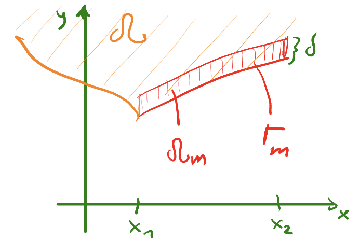
\includegraphics[width=5.96645021645022cm,height=4.03879706152433cm]{k3-1.pdf}}
  \end{itemizedot}
  Beweisstrateige:
  \begin{enumerateroman}
    \item Wir definieren zun{\"a}chst
    \[ \gamma : C^1 (\bar{\Omega}) \rightarrow L^2 (\partial \Omega),
       \text{\quad} v \mapsto v |_{\partial \Omega} \nobracket . \]
    $\gamma$ ist klar linear, und wir sollte noch die Wohldefiniertheit (im
    Sinne von $\gamma (v) \in L^2 (\partial \Omega)$) und die
    Beschr{\"a}nktheit (Stetigkeit) von $\gamma$ bzgl. $H^1$-Norm bei $C^1
    (\bar{\Omega})$ nachweisen.
    
    \item Wir nutzen die Eigenschaft $H^1 (\Omega) = \overline{C^1
    (\bar{\Omega})}^{^{^{\| \bullet \|_{H^1 (\Omega)}}}}$ und erweitern
    $\gamma$ aus i. auf $H^1 (\Omega)$ durch
    \[ \gamma (v) \assign \lim_{n \rightarrow \infty} \gamma (v_n) \]
    f{\"u}r $v \in H^1 (\Omega)$ mit $(v_n)_{n \in \mathbb{N}} \subseteq C^1
    (\bar{\Omega})$ s.d.
    \[ \lim_{n \rightarrow \infty} \| v - v_n \|_{H^1 (\Omega)} = 0. \]
    {\hspace{1.7em}}Dank i. und gilt die Absch{\"a}tzungen mit derselben
    Schranke
    \[ \| \gamma (v) \|_{L^2 (\partial \Omega)} = \lim_{n \rightarrow \infty}
       \| \gamma (v_n) \|_{L^2 (\partial \Omega)} \leqslant C_{\gamma} \lim_{n
       \rightarrow \infty} \| v_n \|_{H^1 (\Omega)} = C_{\gamma} \| v \|_{H^1
       (\Omega)} \]
    und dies zeigt die Wohldefiniertheit von $\gamma$.
  \end{enumerateroman}
  Also bleibt es noch zu zeigen
  \[ \exists C_{\gamma} \in \mathbb{R}_+ \forall v \in C^1 (\bar{\Omega}) :
     \text{\quad} \| \gamma (v) \|_{L^2 (\partial \Omega)} \leqslant
     C_{\gamma} \| v \|_{H^1 (\Omega)} . \text{\qquad} \]
  Dazu:
  \begin{enumeratealpha}
    \item Sei $v \in C^1 (\bar{\Omega})$ und wir betrachten zun{\"a}chst $v
    |_{\Gamma_m} \nobracket$ f{\"u}r $\partial \Omega = \bigcup_{m = 1}^n
    \Gamma_m$.
    
    $\Gamma_m$ ist der Graph einer Funktion $\phi_m \in C^1 ([x_1, x_2])$
    sowie $\Omega^{\delta}_m \subseteq \Omega$ (siehe Anfang des Beweises).
    
    F{\"u}r $x \in [x_1, x_2]$ erhalten wir mittels Integraldarstellung
    \[ \forall t \in [0, s] : \text{\quad} v (x, \phi_m (x)) = v (x, \phi_m
       (x) + t) - \int_{[0, t]} \partial_y v (x, \phi_m (x) + s) \mathd
       \lambda (s) . \]
    {\hspace{1.7em}}Integration obiger Gleichung {\"u}ber $t$ von $0$ bis
    $\delta$ ergibt
    \begin{eqnarray*}
      \delta v (x, \phi_m (x)) & = & \int_{[0, \delta]} v (x, \phi_m (x) + t)
      \mathd \lambda (t)\\
      &  & \text{{\hspace{3em}}} - \int_{[0, \delta]} \int_{[0, t]}
      \partial_y v (x, \phi_m (x) + s) \mathd \lambda (s) \mathd \lambda (t) .
    \end{eqnarray*}
    \item Beim 2. Integral ist der Integrationsbereich ein
    Dreieck-Normalbereich, und d.h. wir k{\"o}nnen das 2. Integral umschreiben
    \
    \[ \begin{array}{ll}
         & \int_{[0, \delta]} \int_{[0, t]} \partial_y v (x, \phi_m (x) + s)
         \mathd \lambda (s) \mathd \lambda (t)\\
         = & \int_{[0, \delta]} \int_{[0, s]} \partial_y v (x, \phi_m (x) + s)
         \mathd \lambda (t) \mathd \lambda (s)\\
         = & \int_{[0, \delta]} (\delta - s) \partial_y v (x, \phi_m (x) + s)
         \mathd \lambda (s)
       \end{array} \]
    also erhalten wir
    \begin{eqnarray}
      \delta v (x, \phi_m (x)) & = & \int_{[0, \delta]} v (x, \phi_m (x) + t)
      \mathd \lambda (t) \nonumber\\
      &  & \text{{\hspace{3em}}} - \int_{[0, \delta]} (\delta - s) \partial_y
      v (x, \phi_m (x) + s) \mathd \lambda (s) . 
    \end{eqnarray}
    \item Wegen Young'sche Ungleichung mit $\varepsilon = 1$ f{\"u}r $p = 2$,
    also $a b \leqslant \frac{1}{2} a^2 + \frac{1}{2} b^2$, gilt
    \[ (a^2 + b^2) = a^2 + 2 a b + b^2 \leqslant a^2 + 2 \left( \frac{1}{2}
       a^2 + \frac{1}{2} b^2 \right) + b^2 = 2 a^2 + 2 b^2 \]
    und dies angewandt auf Quadrat von (3.1) ergibt
    \begin{eqnarray*}
      \delta^2 v (x, \phi_m (x))^2 & \leqslant & 2 \left( \int_{[0, \delta]} v
      (x, \phi_m (x) + t) \mathd \lambda (t) \right)^2\\
      &  & \text{\qquad} + 2 \left( \int_{[0, \delta]} (\delta - s)
      \partial_y v (x, \phi_m (x) + s) \mathd \lambda (s) \right)^2 .
    \end{eqnarray*}
    \item Anwendung von Cauchy-Schwarz auf beide rechte Terme in c) ergibt
    \begin{eqnarray*}
      &  & 2 \left( \int_{[0, \delta]} v (x, \phi_m (x) + t) \mathd \lambda
      (t) \right)^2\\
      & \leqslant & 2 \left( \left( \int_{[0, \delta]} 1^2 \mathd \lambda (t)
      \right)^{\frac{1}{2}} \left( \int_{[0, \delta]} v (x, \phi_m (x) + t)^2
      \mathd \lambda (t) \right)^{\frac{1}{2}} \right)^2\\
      & = & 2 \hspace{4em} \delta \hspace{4em} \int_{[0, \delta]} v (x,
      \phi_m (x) + t)^2 \mathd \lambda (t)
    \end{eqnarray*}
    sowie
    \begin{eqnarray*}
      &  & 2 \left( \int_{[0, \delta]} (\delta - s) \partial_y v (x, \phi_m
      (x) + s) \mathd \lambda (s) \right)^2\\
      & \leqslant & 2 \left( \left( \int_{[0, \delta]} (\delta - s)^2 \mathd
      \lambda (s) \right)^{\frac{1}{2}} \left( \int_{[0, \delta]} (\partial_y
      v (x, \phi_m (x) + s))^2 \mathd \lambda (s) \right)^{\frac{1}{2}}
      \right)^2\\
      & = & 2 \hspace{1.5em} \int_{[0, \delta]} (\delta - s)^2 \mathd \lambda
      (s) \qquad \int_{[0, \delta]} (\partial_y v (x, \phi_m (x) + s))^2
      \mathd \lambda (s)\\
      & = & 2 \hspace{4em} \frac{1}{3} \delta^3 \hspace{5em} \int_{[0,
      \delta]} (\partial_y v (x, \phi_m (x) + s))^2 \mathd \lambda (s) .
    \end{eqnarray*}
    \item Einsetzen von d) in c) liefert
    \[ \delta^2 v (x, \phi_m (x))^2 \leqslant 2 \delta \int_{[0, \delta]} v
       (x, \phi_m (x) + t)^2 \mathd \lambda (t) + \frac{2}{3} \delta^3
       \int_{[0, \delta]} \partial_y v (x, \phi_m (x) + s)^2 \mathd \lambda
       (s) \]
    und mit Division durch $\delta^2$ und dann Integration bzgl. $x$ erhalten
    wir
    \begin{eqnarray*}
      &  & \int_{[x_1, x_2]} v (x, \phi_m (x))^2 \mathd \lambda (x)\\
      & \leqslant & \frac{2}{\delta} \int_{\Omega^{\delta}_m} v (x, y)^2
      \mathd \lambda (x) \mathd \lambda (y) + \frac{2}{3} \delta
      \int_{\Omega^{\delta}_m} (\partial_y v (x, y))^2 \mathd \lambda (x)
      \mathd \lambda (y)\\
      & \leqslant & \max \left\{ \frac{2}{\delta}, \frac{2}{3} \delta
      \right\} \int_{\Omega^{\delta}_m} v^2 + \partial_y v^2 \mathd
      \lambda^2\\
      & \leqslant & \max \left\{ \frac{2}{\delta}, \frac{2}{3} \delta
      \right\} \int_{\Omega^{\delta}_m} v^2 + \partial_y v^2 + \partial_x v^2
      \mathd \lambda^2\\
      & = & \max \left\{ \frac{2}{\delta}, \frac{2}{3} \delta \right\} \| v
      \|^2_{H^1 (\Omega)}\\
      & \backassign & \text{{\hspace{3em}}} \xi \text{{\hspace{2.7em}}} \| v
      \|^2_{H^1 (\Omega)} .
    \end{eqnarray*}
    \item  $\Gamma_m$ ist der Graph einer Funktion $\phi_m \in C^1 ([x_1,
    x_2])$, und daher
    \begin{eqnarray*}
      \int_{\Gamma_m} v^2 \mathd \lambda & = & \int_{[x_1, x_2]} v (x, \phi_m
      (x))^2 \sqrt{1 + \phi_m' (x)^2} \mathd \lambda (x)\\
      & \leqslant & \left\| \sqrt{1 + \phi_m' (x)^2} \right\|_{L^{\infty}
      ([x_1, x_2])} \int_{[x_1, x_2]} v (x, \phi_m (x))^2 \mathd \lambda (x)\\
      & \backassign & \text{{\hspace{5em}}} C_m \hspace{4.5em} \int_{[x_1,
      x_2]} v (x, \phi_m (x))^2 \mathd \lambda (x)
    \end{eqnarray*}
    und somit folgt dank e)
    \[ \int_{\Gamma_m} v^2 \mathd \lambda \leq C_m \xi \| v \|^2_{H^1
       (\Omega)} . \]
    \item Insgesamt erhalten wir
    \begin{eqnarray*}
      \| \gamma (v) \|^2_{L^2 (\partial \Omega)} & \leqslant & \sum_{m = 1}^n
      \int_{\Gamma_m} v^2 \mathd \lambda \leq \sum_{m = 1}^n C_m \xi \| v
      \|^2_{H^1 (\Omega)}
    \end{eqnarray*}
    und d.h. mit $C_{\gamma} \assign \left( \sum_{m = 1}^n C_m \xi
    \right)^{\frac{1}{2}}$ ist $\gamma : C^1 (\bar{\Omega}) \rightarrow L^2
    (\partial \Omega), \text{} v \mapsto v |_{\partial \Omega} \nobracket$
    beschr{\"a}nkt durch \
    \[ \| \gamma (v) \|_{L^2 (\partial \Omega)} \leqslant C_{\gamma} \| v \|
       _{H^1 (\Omega)} . \]
  \end{enumeratealpha}
\end{proof}

\begin{definition}
  \tmtextbf{(Sobolev-Dualr{\"a}ume)}
  
  \tmtextit{F{\"u}r $p \in [1, \infty)$ bezeichnen wir mit
  \[ H^{- m, p} (\Omega) \assign (H^{m, p }_0 (\Omega))' \]
  den Dualraum von $H^{m, p}_0 (\Omega)$. Wir schreiben $H^{- m} (\Omega)
  \assign H^{- m, 2} (\Omega)$.}
\end{definition}

Damit kann man DGL betrachten, deren rechte Seite Funktionale statt Funktionen
sind (Details sp{\"a}ter).

Im Folgenden sehen wir, dass R{\"a}ume $H_0^{m_1, p_1} (\Omega)$ stetig in
$H_0^{m_2, p_2} (\Omega)$ eingebettet werden k{\"o}nnen, falls $m_1, m_2, p_1,
p_2$ geeignet gew{\"a}hlt sind. Weiter lassen sich diese in klassische
H{\"o}lderr{\"a}ume $C^{m, \alpha} (\bar{\Omega})$ einbetten, damit sind
$H^{m, p} (\Omega)$-Funktionen also ,,klassisisch`` differenzierbar.

\begin{theorem}
  \tmtextbf{(1. Sobolev'scher Einbettungssatz)}
  
  \tmtextit{Sei $\Omega \subseteq \mathbb{R}^d$ offen \& beschr{\"a}nkt. Sei
  $m_1, m_2 \in \mathbb{N}_0$ mit $m_1 \geqslant m_2$, und $p_1, p_2 \in [1,
  \infty)$.
  
  Falls $m_1 - \frac{d}{p_1} \geqslant m_2 - \frac{d}{p_2}$ gilt, so
  existiert eine stetige Einbettung
  \[ \mathcal{J} : H^{m_1, p_1}_0 (\Omega) \longhookrightarrow H_0^{m_2, p_2}
     (\Omega) \]
  insb. gilt
  \[ \exists C \geqslant 0 \forall u \in H_0^{m_1, p_1} (\Omega) :
     \text{\quad} \| \mathcal{J} u \|_{H^{m_2, p_2} (\Omega)} \leqslant C \| u
     \|_{H^{m_1, p_1} (\Omega)} . \text{\quad} \]
  {\hspace{1.7em}}Falls $\Omega$ ein Lipschitz-Gebiet ist, dann l{\"a}sst sich
  $\mathcal{J}$ auf $H^{m_1, p_1} (\Omega)$ zu $H^{m_2, p_2} (\Omega)$ stetig
  erweitern. }
\end{theorem}

F{\"u}r den Beweis verweisen wir auf Alt. Satz 8.9.

\begin{theorem}
  \tmtextbf{(2. Sobolev'scher Einbettungssatz)}
  
  \tmtextit{Sei $\Omega \subseteq \mathbb{R}^d$ offen \& beschr{\"a}nkt. Sei
  $m, k \in \mathbb{N}_0$ mit $m \geqslant k$, und $p \in [1, \infty)$.
  
  Falls es ein $\alpha \in (0, 1)$ existiert, s.d. $m - \frac{d}{p} \geqslant
  k + \alpha$ gilt, dann existiert eine stetige Einbettung
  \[ \mathcal{J} : H^{m , p}_0 (\Omega) \longhookrightarrow C^{m, \alpha}
     (\bar{\Omega}) \]
  insb. gilt
  \[ \exists C \geqslant 0 \forall u \in H_0^{m, p} (\Omega) : \text{\quad} \|
     \mathcal{J} u \|_{C^{m, \alpha} (\bar{\Omega})} \leqslant C \| u
     \|_{H^{m, p} (\Omega)} . \text{\quad} \]
  {\hspace{1.7em}}Falls $\Omega$ ein Lipschitz-Gebiet ist, dann l{\"a}sst sich
  $\mathcal{J}$ auf $H^{m, p} (\Omega)$ stetig erweitern. }
\end{theorem}

F{\"u}r den Beweis verweisen wir auf Alt. Satz 8.13.

\begin{remark*}
  \
  
  F{\"u}r einen Sobolev-Raum $H^{m, p} (\Omega)$ mit $\Omega \subseteq
  \mathbb{R}^d$ nennen wir die Gr{\"o}{\ss}e $m - \frac{d}{p}$ den
  \tmtextit{{\underline{Sobolev-Index}}}. Dies ist offenbar wichtig, denn dies
  charakterisiert die Regularit{\"a}t von Sobolev-Funktionen. 
\end{remark*}

\begin{corollary}
  \tmtextbf{(Stetigkeit von $H_0^1 (\Omega)$-Funktion f{\"u}r $d = 1$)}
  
  \tmtextit{Sei $d = 1$, d.h. $\Omega \subseteq \mathbb{R}$, dann hat jedes $u
  \in H_0^1 (\Omega)$ einen stetigen Repr{\"a}sentant.}
\end{corollary}

\begin{proof}
  \
  
  Mit $\alpha \leqslant \frac{1}{2}$, $k = 0$, $p = 2$ und $m = 1$ gilt $m -
  \frac{d}{p} > 1 - \frac{1}{2} = \frac{1}{2} \geqslant \alpha = \alpha + k$,
  also existiert nach Satz 3.12 eine stetige Einbettung $\mathcal{J} : H_0^1
  (\Omega) \longhookrightarrow C^{0, \alpha} (\bar{\Omega})$. Das bedeutet,
  f{\"u}r jedes $u \in H_0^1 (\Omega)$ ist $\mathcal{J} u \in C^{0, \alpha}
  (\Omega)$ mit $u = \mathcal{J} u$ f.{\"u}..
  
  Wegen Satz 2.4 Schachtelung der H{\"o}lderr{\"a}ume ist also $\mathcal{J} u
  \in C^0 (\Omega) $.
\end{proof}

\begin{remark*}
  {\tmdummy}
  
  \begin{itemizedot}
    \item F{\"u}r $d > 1$ ist dies falsch: $m - \frac{d}{p} = 1 - \frac{d}{2}
    \leqslant 0$ ist nie gr{\"o}{\ss}er gleich $k + \alpha$ f{\"u}r $\alpha
    \in (0, 1)$, also Satz 3.12 nicht anwendbar.
    
    \item F{\"u}r $d > 1$ enth{\"a}lt $H^1 (\Omega)$ tats{\"a}chlich
    Funktionen mit Punktsingularit{\"a}ten, z.B.:
    \begin{itemizeminus}
      \item im Fall $d = 2$: \text{\quad}$u (x) = \log \left( \log \left(
      \frac{2}{\| x \|} \right) \right) \in H^1 (B_1 (0))$
      
      \item im Fall $d \geqslant 3$: \text{\quad}$u (x) = \| x \|^{- \beta}
      \in H^1 (B_1 (0))$ f{\"u}r $\beta \in \left( 0, \frac{d - 2}{2}
      \right)$.
    \end{itemizeminus}
  \end{itemizedot}
\end{remark*}

\begin{theorem}
  \tmtextbf{(Poincar{\'e}-Friedrich)}
  
  \tmtextit{Sei $\Omega \subseteq \mathbb{R}^d$ offen und beschr{\"a}nkt,
  sowie $s \assign \tmop{diam} (\Omega)$.
  
  Dann gilt
  \[ \forall v \in H^1_0 (\Omega) : \text{\quad} \| v \|_{L^2 (\Omega)}
     \leqslant s | v |_{H^1 (\Omega)} . \text{\quad} \]}
\end{theorem}

\begin{proof}
  (Argument f{\"u}r $d = 1$ und $v \in C^1$ schon in Bew. 1.41. gesehen)
  
  Da $C^{\infty}_0 (\Omega)$ dicht in $H^1_0 (\Omega)$ ist (Satz von
  Meyers-Serrin), gen{\"u}gt es, Ungleichung f{\"u}r $v \in C^{\infty}_0
  (\Omega)$ zu zeigen.
  
  OBdA sei das Koordinatensystem so verschoben, dass es gilt
  \[ \Omega \subseteq [0, s]^d . \]
  also ist jedes $v \in C^{\infty}_0 (\Omega)$ auf $R \assign [0, s]^d$ durch
  $0$ fortsetzbar, und es gilt f{\"u}r jedes $v \in C^{\infty}_0 (\Omega)$ und
  jedes $x = (x_1, \ldots, x_d) \in R$
  \begin{eqnarray*}
    v (x_1, \ldots, x_d) & = & v (0, x_2, \ldots, x_d) + \int_{[0, x_1]}
    \partial_{x_1} v (t, x_2, \ldots, x_d) \mathd \lambda (t)\\
    & = & \text{{\hspace{3em}}} 0 \hspace{3em} + \int_{[0, x_1]}
    \partial_{x_1} v (t, x_2, \ldots, x_d) \mathd \lambda (t) .
  \end{eqnarray*}
  {\hspace{1.7em}}Damit erhalten wir
  \begin{eqnarray*}
    | v (x) |^2 & = & \left| \int_{[0, x_1]} 1 \cdot \partial_{x_1} v (t, x_2,
    \ldots, x_d) \mathd \lambda (t) \right|^2\\
    & \leqslant & \int_{[0, x_1]} 1^2 \mathd t \cdot \int_{[0, x_1]} |
    \partial_{x_1} v (t, x_2, \ldots, x_d) |^2 \mathd \lambda (t)\\
    & = & \text{\qquad} s \hspace{1.7em} \cdot \int_{[0, x_1]} |
    \partial_{x_1} v (t, x_2, \ldots, x_d) |^2 \mathd \lambda (t)\\
    & \leqslant & \text{\qquad} s \hspace{1.7em} \cdot \int_{[0, s]} |
    \partial_{x_1} v (t, x_2, \ldots, x_d) |^2 \mathd \lambda (t)
  \end{eqnarray*}
  wobei die zweite Zeile aus Cauchy-Schwarz folgt, und damit folgt
  \begin{eqnarray*}
    \int_{[0, s]} | v (x_1, \ldots, x_d) |^2 \mathd \lambda (x_1) & \leqslant
    & \int_{[0, s]} \text{} s \int_{[0, s]} | \partial_{x_1} v (t, x_2,
    \ldots, x_d) |^2 \mathd \lambda (t) \mathd \lambda (x_1)\\
    & = & s^2 \int_{[0, s]} | \partial_{x_1} v (t, x_2, \ldots, x_d) |^2
    \mathd \lambda (t)
  \end{eqnarray*}
  da das innere Integral auf der rechten Seite unabh{\"a}ngig von $x_1$ ist.
  
  Integration {\"u}ber andere Koordinaten ergibt
  \begin{equation}
    \int_R | v (x) |^2 \mathd \lambda^d (x) \leqslant s^2 \int_R
    (\partial_{x_1} v (x))^2 \mathd \lambda^d (x) \leqslant s^2 \int_R \|
    \nabla v (x) \|^2 \mathd \lambda^d (x)
  \end{equation}
  wobei die Absch{\"a}tzung aus der zweite Zeile aus der Definition von
  $\nabla v$ folgt, und per Definition dann
  \[ \| v \|_{L^2}^2 = \int_R | v (x) |^2 \mathd \lambda^d (x) \leqslant s^2
     \int_R \| \nabla v (x) \|^2 \mathd \lambda^d (x) = s^2 | v |^2_{H^1} . \]
\end{proof}

\begin{corollary}
  \tmtextbf{(Norm{\"a}quivalenz auf $H^m_0 (\Omega)$)}
  
  \tmtextit{Sei $\Omega \subseteq \mathbb{R}^d$ offen \& beschr{\"a}nkt mit
  $\tmop{diam} (\Omega) \leqslant s$.
  
  Dann sind in $H^m_0 (\Omega)$ die Norm $\| \bullet \|_{H^m (\Omega)}$ und
  Seminorm $| \bullet |_{H^m (\Omega)}$ {\"a}quivalent mit
  \begin{equation}
    \forall v \in H^m_0 (\Omega) : \text{\quad} | v |_{H^m (\Omega)} \leqslant
    \| v \|_{H^m (\Omega)} \leqslant (1 + s)^m | v |_{H^m (\Omega)} . \quad
  \end{equation}}
\end{corollary}

\begin{proof}
  \
  
  Die linke Seite von (3.3) ist klar, und die rechte Seite zeigen wir mit
  vollst{\"a}ndiger Induktion.
  
  Beim I.A. $m = 0$ ist $| \bullet |_{H^0} = \| \bullet \|_{L^2}$ und $(1 +
  s)^0 = 1$, also (3.3) gilt mit Gleichheit.
  
  Nun zum I.S. $m - 1 \rightarrow m$:
  
  Gelte die Behauptung f{\"u}r $m - 1$, dann gilt f{\"u}r jedes $v \in H^m_0
  (\Omega)$: \
  \[ \| v \|^2_{H^m (\Omega)} = \| v \|^2_{H^{m - 1}} (\Omega) + | v |^2_{H^m
     (\Omega)} \leqslant (1 + s)^{2 (m - 1)} | v |^2_{H^{m - 1} (\Omega)} + |
     v |^2_{H^m (\Omega)} \]
  wobei wir uns daran erinnern, dass
  \[ | v |^2_{H^{m - 1} (\Omega)} = \sum_{| \beta | = m - 1} \|
     \partial^{\beta} v \|^2_{L^2 (\Omega)} . \]
  {\hspace{1.7em}}F{\"u}r jedes $\beta \in \mathbb{N}_0^d$ mit $| \beta |
  \leqslant m - 1$ wenden wir die erste Ungleichheit in (3.2) auf
  $\partial^{\beta} v$ an und erhalten
  \[ \| \partial^{\beta} v \|_{L^2 (\Omega)} \leqslant s \| \partial_{x_1}
     \partial^{\beta} v \|_{L^2 (\Omega)} \]
  und somit
  \begin{eqnarray*}
    \| v \|^2_{H^m (\Omega)} & \leqslant & (1 + s)^{2 (m - 1)} s^2 \sum_{|
    \beta | = m - 1} \| \partial_{x_1} \partial^{\beta} v \|^2_{L^2 (\Omega)}
    + | v |^2_{H^m (\Omega)}\\
    & \leqslant & (1 + s)^{2 (m - 1)} s^2 \enspace \sum_{| \beta | = m} \|
    \partial^{\beta} v \|^2_{L^2 (\Omega)} \enspace + | v |^2_{H^m (\Omega)}\\
    & = & (1 + s)^{2 (m - 1)} s^2 \enspace \sum_{| \beta | = m} \|
    \partial^{\beta} v \|^2_{L^2 (\Omega)} \enspace + \sum_{| \beta | = m} \|
    \partial_{x_1} \partial^{\beta} v \|^2_{L^2 (\Omega)}\\
    & = & ((1 + s)^{2 (m - 1)} s^2 + 1) \sum_{| \beta | = m} \|
    \partial^{\beta} v \|^2_{L^2 (\Omega)} .
  \end{eqnarray*}
  {\hspace{1.7em}}Mit
  \begin{eqnarray*}
    (1 + s)^{2 m} & = & (1 + s)^{2 (m - 1)} (1 + s)^2\\
    & = & s^2 (1 + s)^{2 (m - 1)} + 2 s (1 + s)^{2 (m - 1)} + (1 + s)^{2 (m -
    1)}\\
    & \geqslant & (1 + s)^{2 (m - 1)} s^2 + 1
  \end{eqnarray*}
  folgt daher
  \[ \| v \|^2_{H^m (\Omega)} \leqslant (1 + s)^{2 m} \sum_{| \beta | = m} \|
     \partial^{\beta} v \|^2_{L^2 (\Omega)} = (1 + s)^{2 m} | v |^2_{H^m
     (\Omega)} . \]
\end{proof}

\

\section{Schwache L{\"o}sungen f{\"u}r elliptische PDEs}

Wir illustrieren die \tmtextbf{Idee} mitttels eines Poisson-RWP mit
Nullrandwerten, also
\[ \begin{array}{lllll}
     - \Delta u & = & f &  & \text{in } \Omega\\
     u & = & 0 &  & \text{auf } \partial \Omega
   \end{array} \]
f{\"u}r $\Omega \subseteq \mathbb{R}^d$ offen \& beschr{\"a}nkt und $f \in C
(\Omega)$.

PDE in solcher Darstellung nennt man ,,{\underline{\tmtextit{starke Form der
PDE}}}``.

Sei $u \in C^2 (\Omega) \cap C^0 (\bar{\Omega})$ eine klassische L{\"o}sung
zum Poisson-RWP.

Durch Multiplizieren mit einer Testfunktion $v \in C^1_0 (\bar{\Omega})$ und
dann Integrieren erhalten wir
\[ - \int_{\Omega} \Delta u \cdot v \mathd \lambda^d = \int_{\Omega} f \cdot
   v \mathd \lambda^d \]
und mit partieller Integration folgt
\[ - \int_{\Omega} \Delta u \cdot v \mathd \lambda^d = \int_{\Omega} \nabla u
   \bullet \nabla v \mathd \lambda^d - \int_{\partial \Omega} (\nabla u
   \bullet n) v \mathd \lambda^{d - 1} = \int_{\Omega} \nabla u \bullet \nabla
   v \mathd \lambda^d - 0 \]
da $v \in C^1_0 (\bar{\Omega})$.

D.h., die klassische L{\"o}sung $u$ l{\"o}st auch die ,,schwache Form der
PDE``
\begin{equation}
  \forall v \in C^1_0 (\Omega) : \text{\quad} \int_{\Omega} \nabla u \bullet
  \nabla v \mathd \lambda^d = \int_{\Omega} f \cdot v \mathd \lambda^d .
  \text{\quad}
\end{equation}
{\hspace{1.7em}}Hierzu bemerken wir:
\begin{itemizedot}
  \item Terme in (3.4) machen Sinn f{\"u}r $u \in C^1_0 (\Omega)$ oder $u \in
  H^1_0 (\Omega)$, daher macht es Sinn, nach ,,schwachen L{\"o}sungen``, d.h.
  L{\"o}sung von (3.4) zu suchen.
  
  \item Eine klassische L{\"o}sung ist also eine schwache L{\"o}sung.
  
  \item F{\"u}r allgemeinere $f$, z.B. unstetige, kann es vorkommen, dass
  keine klassische L{\"o}sung, aber schwache L{\"o}sung $u \in H^1_0 (\Omega)$
  existiert.
  
  \item Durch eine Bilinearform
  \[ a (u, v) \assign \int_{\Omega} \nabla u \bullet \nabla v \mathd
     \lambda^d \]
  und eine Linearform
  \[ L_f (v) \assign \int_{\Omega} f \cdot v \mathd \lambda^d \]
  kann (3.4) umgeschrieben werden als
  \[ \forall v \in H^1_0 (\Omega) : \text{\quad} a (u, v) = L_f (v) .
     \text{\quad} \]
  Wegen Approximierbarkeit von $H^1_0 (\Omega)$ bzw. $C^1_0 (\Omega)$ durch
  $C^{\infty}_0$-Funktionen ist es egal, ob $\forall v \in C^1_0 (\Omega)$
  oder $\forall v \in H^1_0 (\Omega)$ gefordert wird.
  
  \item Interessanten Fragen dabei geh{\"o}ren u.a. Existenz \&
  Eindeutigkeit, Stabilit{\"a}t \& Regularit{\"a}t solcher schwachen
  L{\"o}sungen. 
\end{itemizedot}
\begin{definition}
  \tmtextbf{(Stetigkeit)}
  
  \tmtextit{Sei $V$ ein reeller Hilbertraum mit induzierter Norm $\| \bullet
  \|$.
  
  Eine {\underline{Bilinearform}} $a : V \times V \rightarrow \mathbb{R}$
  hei{\ss}t {\underline{stetig}} mit {\underline{Stetigkeitskonstante
  $\gamma_a \in \mathbb{R}$}}, g.d.w. es gilt
  \[ \sup_{u, v \in V \backslash \{ 0 \}} \frac{| a (u, v) |}{\| u \| \cdot
     \| v \|} \backassign \gamma_a < \infty . \]
  {\hspace{1.7em}}Eine {\underline{Linearform}} $L : V \rightarrow \mathbb{R}$
  hei{\ss}t {\underline{stetig}}, g.d.w. es gilt
  \[ \| L \|_{V'} \assign \sup_{v \in V \backslash \{ 0 \}} \frac{| L (v)
     |}{\| v \|} < \infty . \]}
\end{definition}

\begin{remark*}
  \
  
  Also ist z.B. das Skalarprodukt stetig mit $\gamma_{\langle \bullet,
  \bullet \rangle} = 1$, denn mit Cauchy-Schwarz gilt f{\"u}r jedes $u, v \in
  V$: $\langle u, v \rangle \leqslant \| u \| \cdot \| v \|$, und somit
  f{\"u}r $u, v \in V \backslash \{ 0 \}$: $\frac{| \langle u, v \rangle |}{\|
  u \| \cdot \| v \|} \leqslant 1$ und Gleichheit nur bei $u = v$.
\end{remark*}

Wir definieren noch einen Begriff f{\"u}r ,,Beschr{\"a}nkung nach unten``:

\begin{definition}
  \tmtextbf{(Koerzivit{\"a}t)}
  
  \tmtextit{Sei $V$ ein reeller Hilbertraum mit induzierter Norm $\| \bullet
  \|$.
  
  Eine Bilinearform $a : V \times V \rightarrow \mathbb{R}$ hei{\ss}t
  {\underline{koerziv}} mit {\underline{Koerzivit{\"a}tskonstante $\alpha_a
  \in \mathbb{R}$}}, g.d.w. es gilt
  \[ \inf_{u \in V \backslash \{ 0 \}} \frac{a (u, u)}{\| u \| \cdot \| u \|}
     \backassign \alpha_a > 0. \]}
\end{definition}

\begin{remark*}
  {\tmdummy}
  
  \begin{itemizedot}
    \item F{\"u}r eine Bilinearform $a : V \times V \rightarrow \mathbb{R}$
    ist ihre Koerzivit{\"a}tskonstante kleiner gleich ihrer
    Stetigkeitskonstante, da
    \[ \alpha_a = \inf_{u \in V \backslash \{ 0 \}} \frac{a (u, u)}{\| u \|
       \cdot \| u \|} \leqslant \sup_{u \in V \backslash \{ 0 \}} \frac{| a
       (u, u) |}{\| u \| \cdot \| u \|} \leqslant \sup_{u, v \in V \backslash
       \{ 0 \}} \frac{| a (u, v) |}{\| u \| \cdot \| v \|} = \gamma_a . \]
    \item Man sieht leicht, dass ein Skalarprodukt $\langle \bullet, \bullet
    \rangle$ koerziv mit $\alpha_{\langle \bullet, \bullet \rangle} = 1$ ist.
    
    \item Eine Bilinearform $a : V \times V \rightarrow \mathbb{R}$ ist
    koerziv g.d.w. ihr symmetrischer Anteil $a_s (u, v)$ koerziv ist, da mit
    $a_s (u, v) \assign \frac{1}{2} (a (u, v) + a (v, u))$ ist $a (u, u) = a_s
    (u, u)$.
    
    \item $\gamma_a$, $\alpha_a$ lassen sich durch geeignete EWP / SVD
    berechnen. 
  \end{itemizedot}
\end{remark*}

\begin{definition}
  \tmtextbf{(Bilinearform / Linearform f{\"u}r elliptische PDEs)}
  
  \tmtextit{Sei $\Omega \subseteq \mathbb{R}^d$ beschr{\"a}nkt und eine
  elliptische PDE mit Nullrandwerten gegeben durch
  \[ \begin{array}{lllll}
       - \nabla \bullet (A \nabla u) + \nabla \bullet (b u) + c u & = & f &  &
       \text{in } \Omega\\
       u & = & 0 &  & \text{auf } \partial \Omega
     \end{array} \]
  mit $A (x) = (a_{i j} (x))_{i, j = 1}^d \in (L^{\infty} (\Omega))^{d \times
  d}$, $b (x) = (b_i (x))_{i = 1}^d \in (L^{\infty} (\Omega))^d$, $c \in
  L^{\infty} (\Omega)$ und $f \in L^2 (\Omega)$.
  
  Dann definieren wir f{\"u}r $u, v \in H^1 (\Omega)$
  \[ a (u, v) \assign \int_{\Omega} (A \nabla u) \bullet \nabla v - (b \bullet
     \nabla v) u + c u v \mathd \lambda^d \]
  \[ L_f (v) \assign \int_{\Omega} f v \mathd \lambda^d . \]}
\end{definition}

\begin{theorem}
  \tmtextbf{(Stetigkeit \& Koerzivit{\"a}t f{\"u}r $b = 0$ und $c = 0$)}
  
  \tmtextit{Sei $A$ {\underline{gleichm{\"a}{\ss}ig elliptisch}}, d.h.
  \[ \exists \tilde{\alpha} \in \mathbb{R}_+ \forall x \in \Omega \forall z
     \in \mathbb{R}^d : \text{\qquad} \langle z, A (x) z \rangle_2 \geqslant
     \tilde{\alpha} \| z \|^2_2 \]
  und {\underline{gleichm{\"a}{\ss}ig beschr{\"a}nkt}} d.h.
  \[ \exists C \in \mathbb{R}_+ \exists \text{Matrixnorm } \| \bullet
     \|_{\sim}  \text{auf } \mathbb{R}^{d \times d} \forall x \in \Omega :
     \text{\qquad} \| A (x) \|_{\sim} \leqslant C. \]
  \text{{\hspace{1.7em}}}Sei zudem $b = 0$ und $c = 0$.
  
  Dann ist die Bilinearform $a (u, v)$ aus 3.18 {\underline{stetig auf $H^1
  (\Omega)$}} und {\underline{koerziv auf $H^1_0 (\Omega)$}}. \ }
\end{theorem}

\begin{proof}
  Zur Stetigkeit auf $H^1 (\Omega)$:
  
  F{\"u}r $u, v \in H^1 (\Omega)$ gilt:
  \begin{eqnarray*}
    a (u, v) = \int_{\Omega} (A \nabla u) \bullet \nabla v \mathd \lambda^d &
    \leqslant & \int_{\Omega} \| A \nabla u \|_2 \cdot \| \nabla v \|_2 \mathd
    \lambda^d\\
    & \leqslant & \int_{\Omega} \| A \|_2 \cdot \| \nabla u \|_2 \cdot \|
    \nabla v \|_2 \mathd \lambda^d\\
    & \leqslant & \int_{\Omega} C' \cdot {\| A \|_{\sim}}  \cdot \| \nabla u
    \|_2 \cdot \| \nabla v \|_2 \mathd \lambda^d\\
    & \leqslant & \int_{\Omega} C' C  \cdot \| \nabla u \|_2 \cdot \| \nabla
    v \|_2 \mathd \lambda^d\\
    & = : & \int_{\Omega} \text{\enspace} \tilde{C} \enspace  \cdot \| \nabla
    u \|_2 \cdot \| \nabla v \|_2 \mathd \lambda^d\\
    & \leqslant & \tilde{C} \int_{\Omega} \| \nabla u \|^2_2 \mathd \lambda^d
    \cdot \int_{\Omega} \| \nabla v \|^2_2 \mathd \lambda^d\\
    & = & \widetilde{C} \text{{\hspace{1.2em}}} | u |_{H^1 (\Omega)}
    \hspace{1.2em} \cdot \text{{\hspace{1.65em}}} | v |_{H^1 (\Omega)}\\
    & \leqslant & \tilde{C} \quad \| u \|_{H^1 (\Omega)} \quad \cdot
    \text{{\hspace{1.4em}}} \| v \|_{H^1 (\Omega)}
  \end{eqnarray*}
  wobei die erste Zeile wegen Cauchy-Schwarz auf Integranden folgt, dritte
  Zeile wegen {\"A}quivalenz von Matrizennormen, 6. Zeile wegen C.S. in $L^2$
  und letzte Zeile per Definition von $H^1 (\Omega)$-Norm.
  
  \qquad Zur Koerzivit{\"a}t auf $H^1_0 (\Omega)$:
  
  Da $\Omega$ beschr{\"a}nkt, schreiben wir $s \assign \tmop{diam} (\Omega)$.
  
  Damit gilt f{\"u}r jedes $u \in H^1_0 (\Omega)$:
  \begin{eqnarray*}
    a (u, u) = \int_{\Omega} (A \nabla u) \bullet \nabla u \mathd \lambda^d &
    \geqslant & \int_{\Omega} \tilde{\alpha} \| \nabla u \|^2 \mathd \lambda^d
    = \tilde{\alpha} | u |^2_{H^1 (\Omega)} \geqslant \frac{\tilde{\alpha}}{(1
    + s)^2} \| u \|^2_{H^1 (\Omega)}
  \end{eqnarray*}
  wobei die erste Ungleichheit aus glm. Elliptizit{\"a}t folgt und die zweite
  wegen Norm{\"a}quivalenz 3.15.
  
  Somit sehen wir
  \[ \alpha_a \assign \inf_{u \in H^1_0 \backslash \{ 0 \}} \frac{a (u,
     u)}{\| u \|^2_{H^1 (\Omega)}} \geqslant \frac{\tilde{\alpha}}{(1 + s)^2}
     > 0. \]
\end{proof}

\begin{remark*}
  {\tmdummy}
  
  \begin{itemizedot}
    \item $a (\bullet, \bullet)$ ist nicht koerziv auf $H^1 (\Omega)$:
    
    W{\"a}hle $u \in H^1 (\Omega)$ konstant, also $u (x) = k$ f{\"u}r ein $k
    \in \mathbb{R}_{\neq 0}$, dann gilt
    \[ \frac{a (u, u)}{\| u  \|^2_{H^1 (\Omega)}} = \frac{0}{\| u  \|^2_{H^1
       (\Omega)}} = 0. \]
    \item Da Stetigkeit sich auf Teilr{\"a}ume vererbt, ist insb. $a (\bullet,
    \bullet)$ stetig auf $H^1_0 (\Omega)$.
    
    \item Da Koerzivit{\"a}t sich auf Teilr{\"a}ume vererbt, ist insb. $a
    (\bullet, \bullet)$ koerziv auf Teilr{\"a}ume von $H^1_0 (\Omega)$.
    
    \item Falls $A$ symmetrisch, so ist $a (\bullet, \bullet)$ symmetrisch.
    
    \item {\"A}hnliche Aussage wie 3.19 gilt falls $b \neq 0$ aber $c > 0$
    ,,gen{\"u}gend gro{\ss}``. In diesem Fall stellt sich kein Problem mit der
    Stetigkeit dar, aber f{\"u}r die Koerzivit{\"a}t wird man sehen, dass im
    Fall $b \neq 0$ gewisse zus{\"a}tzliche Voraussetzung von $c$ verlangt
    werden muss. 
  \end{itemizedot}
\end{remark*}

\begin{remark*}
  \tmtextbf{(Stetigkeit der rechten Seite)}
  
  Die Linearform
  \[ L_f : H^1 (\Omega) \rightarrow \mathbb{R}, v \mapsto \int_{\Omega} f v
     \mathd \lambda^d \]
  ist offensichtlich linear.
  
  Wegen $H^1 (\Omega) \subseteq L^2 (\Omega)$ gilt mit $f \in L^2 (\Omega)$:
  \[ | L_f (v) | = | \langle f, v \rangle_{L^2} | \leqslant \| f \|_{L^2}
     \cdot \| v \|_{L^2} \leqslant \| f \|_{L^2} \cdot \| v \|_{H^1} \]
  also ist $L_f$ stetig auf $H^1 (\Omega)$ und $H^1_0 (\Omega)$.
  
  Falls $v \in H^1_0 (\Omega)$ gilt die Eigenschaft sogar f{\"u}r $L_f$ mit
  allgemeinerem $f$, z.B. mit einem $f \notin L^2 (\Omega)$, solange noch $L_f
  \in (H^1 (\Omega))$. 
\end{remark*}

\begin{definition}
  \tmtextbf{(Energie-Skalarprodukt)}
  
  \tmtextit{Falls $a (\bullet, \bullet)$ bilinear und koerziv, dann ist der
  symmetrische Anteil ein Skalarprodukt, das sogenannte
  {\underline{Energieskalarprodukt}}
  \[ \langle u, v \rangle_a \assign \frac{1}{2} (a (u, v) + a (v, u)) .  \]}
\end{definition}

\begin{remark*}
  {\tmdummy}
  
  \begin{itemizedot}
    \item Dabei sind die Bilinearit{\"a}t und Symmetrie klar. Positive
    Definitheit resultiert genau aus Koerzivit{\"a}t.
    
    \item Damit ergibt sich die f{\"u}r die Fehleranalyse n{\"u}tzliche
    Energienorm
    \[ \| u \|_a \assign \sqrt{\langle u, v \rangle_a} . \]
    \item Es folgt Norm{\"a}quivalenz auf $H^1_0 (\Omega)$ von $\| \bullet
    \|_a$ zu $\| \bullet \|_{H^1}$ (oder $| \bullet |_{H^1}$):
    \[ \alpha \| u \|_{H^1}^2 \leqslant a_s (u, u) = \| u \|_a^2 = a (u, u)
       \leqslant \gamma_a \| u \|^2_{H^1} \]
    wobei die erste Ungleichheit aus Koerzivit{\"a}t und die Zweite aus
    Stetigkeit von $a (\bullet, \bullet)$ folgt. 
  \end{itemizedot}
\end{remark*}

\begin{definition}
  \tmtextbf{(Schwache L{\"o}sung)}
  
  \tmtextit{Seien $a (\bullet, \bullet)$, $L_f (\bullet)$ einer elliptischen
  PDE wie in 3.18 gegeben.
  
  Wir nennen $u \in H^1_0 (\Omega)$ {\underline{schwache L{\"o}sung}} der
  PDE, g.d.w. es gilt
  \[ \forall v \in H^1_0 (\Omega) : \text{\qquad} a (u, v) = L_f (v) . \]}
\end{definition}

\begin{theorem}
  \tmtextbf{(Klassische L{\"o}sung ist schwache L{\"o}sung)}
  
  \tmtextit{Sei $u \in C^2 (\Omega) \cap C^0 (\bar{\Omega})$ klassische
  L{\"o}sung der PDE und $f \in C^0 (\Omega)$.
  
  Dann ist $u$ schwache L{\"o}sung der PDE. }
\end{theorem}

\begin{proof}
  Wie zu Beginn von Abschnitt 3.2: Multiplikation mit $v \in H^1_0 (\Omega)$,
  dann Integration \& partielle Integration{\textdots}
\end{proof}

Wir behandeln im Folgenden die Existenz \& Eindeutigkeit der schwachen
L{\"o}sungen f{\"u}r elliptische PDEs, und zwar zun{\"a}chst zum
Poisson-Problem, dann allgemein.

F{\"u}r die Existenz \& Eindeutigkeit von schwachen L{\"o}sungen der
Poisson-Gleichung ben{\"o}tigen wir zwei Hilfss{\"a}tze:

\begin{theorem}
  \tmtextbf{(Orthogonale Projektion)}
  
  \tmtextit{Sei $V$ ein Hilbertraum und $W \subseteq V$ ein abgeschlossener
  Teilraum.
  
  Dann exisitert genau ein $P : V \rightarrow W$ mit der Eigenschaft
  \[ \forall v \in V \forall w \in W : \text{\qquad} \left\langle v - P
     \text{} v, w \right\rangle = 0. \]
  {\hspace{1.7em}}$P$ ist ein stetiger linearer Operator und zwar die
  sogenannte {\underline{orthogonale Projektion auf $W$}}.}
\end{theorem}

Beweis zu 3.23. wird als {\"U}bung {\"u}berlassen. F{\"u}r $V \cong
\mathbb{C}^m$ siehe auch NUM I, 5.20 \& 5.21.

\begin{theorem}
  \tmtextbf{(Riesz'scher Darstellungssatz)}
  
  \tmtextit{Sei $V$ ein Hilbertraum, so ist die {\underline{Riesz-Abbildung}}
  $\mathcal{J}$ definiert als
  \[ \mathcal{R} : V \rightarrow V', v \mapsto \langle v, \bullet \rangle \]
  eine stetige, lineare, bijektive Isometrie.
  
  Insbesondere exisitert zu jedem $L \in V'$ ein eindeutiger
  {\underline{Riesz-Repr{\"a}sentant}} $v_L \assign \mathcal{R}^{- 1} (L) \in
  V$ mit $L (\bullet) = \langle v_L, \bullet \rangle$.}
\end{theorem}

\begin{proof}
  
  \begin{enumerateroman}
    \item Linearit{\"a}t ist klar.
    
    \item Isometrie folgt aus
    \[ \| \mathcal{R} (v) \| = \sup_{w \in V \backslash \{ 0 \}} \frac{|
       \mathcal{R} (v) (w) |}{\| w \|} = \sup_{w \in V \backslash \{ 0 \}}
       \frac{| \langle v, w \rangle |}{\| w \|} = \frac{| \langle v, v \rangle
       |}{\| v \|} = \frac{\| v \|^2}{\| v \|} = \| v \| \]
    wobei die dritte Gleicheit wegen Cauchy-Schwarz gilt: C.S. liefert eine
    Ungleichung, bei der die Gleicheit g.d.w. beide Terme gleich gilt.
    
    \item Stetigkeit folgt direkt aus Isometrie, also
    \[ \| \mathcal{R} \| = \sup_{v \in V \backslash \{ 0 \}} \frac{\|
       \mathcal{R} (v) \|}{\| v \|} = 1 < \infty . \]
    \item Zur Injektivit{\"a}t:
    
    $\mathcal{R} (v) = 0$ bedeutet $\| \mathcal{R} (v) \| = 0$ und wegen
    Isometrie hei{\ss}t es $\| v \| = 0$ also $v = 0$ und damit ist $\ker
    (\mathcal{R})$ trivial.
    
    \item Zur Surjektivit{\"a}t:
    
    F{\"u}r jedes $L \in V' \backslash \{ 0 \}$ ist $\ker (L)$ abgeschlossen,
    also gibt es nach 3.23 eine orthogonale Projektion $P : V \rightarrow \ker
    (L)$.
    
    Sei $v_0 \in V$ mit $L (v_0) = 1$ und setze $v_1 \assign v_0 - P \text{}
    v_0$.
    
    Es ist $L (v_1) = L (v) = 1$, also $v_1 \neq 0$, und $v_1 \perp \ker (L)$.
    
    Zudem gilt f{\"u}r jedes $v \in V$: $v - L (v) v_1 \in \ker (L)$, und
    damit
    \begin{eqnarray*}
      \left\langle \frac{v_1}{\| v_1 \|^2}, v \right\rangle & = & \left\langle
      \frac{v_1}{\| v_1 \|^2}, v - L (v) v_1 + L (v) v_1 \right\rangle\\
      & = & \left\langle \frac{v_1}{\| v_1 \|^2}, v - L (v) v_1 \right\rangle
      + \left\langle \frac{v_1}{\| v_1 \|^2}, L (v) v_1 \right\rangle\\
      & = & \text{{\hspace{5em}}} 0 \hspace{3.9em} + L (v) \frac{\langle v_1,
      v_1 \rangle}{\| v_1  \|^2}\\
      & = & L (v)
    \end{eqnarray*}
    wobei die dritte Gleicheit aus $v_1 \perp \ker (L)$ folgt.
    
    Daher ist $L = \mathcal{R} \left( \frac{v_1}{\| v_1 \|^2} \right) \in
    \tmop{im} (\mathcal{R})$, also $\mathcal{R}$ surjektiv.
  \end{enumerateroman}
\end{proof}

\begin{corollary}
  \tmtextbf{(Ex. \& Eind. schwacher L{\"o}sung von Poisson-Problem)}
  
  \tmtextit{Betrachte $A (x) = I$, $c (x) = 0$ und $b (x) = 0$ in Def. 3.18,
  also
  \[ \forall v \in H^1_0 (\Omega) : \text{\qquad} a (u, v) = \int_{\Omega}
     \nabla u \bullet \nabla v \mathd \lambda^d \quad \wedge \text{\quad} L_f
     (v) = \int_{\Omega} f v \mathd \lambda^d \]
  f{\"u}r ein beliebiges $f \in L^2 (\Omega)$.
  
  Dann existiert eine eindeutige schwache L{\"o}sung $u \in H^1_0 (\Omega)$
  der Poisson-Gleichung mit Nullrandwerten, d.h.
  \[ \forall v \in H^1_0 (\Omega) : \text{\qquad} a (u, v) = L_f (v) \]
  und es gilt $| u |_{H^1} \leqslant C \| L_f \|_{H^{- 1} (\Omega)}$ mit $C$
  unabh{\"a}ngig von $L_f$. }
\end{corollary}

\begin{proof}
  \
  
  $A (x)$ ist glm. elliptisch \& glm. beschr{\"a}nkt, also ist $a (\bullet,
  \bullet)$ nach 3.19 koerziv \& stetig auf $H^1_0 (\Omega)$.
  
  Zudem ist $a (\bullet, \bullet)$ symmetrisch, also genau das
  Energie-Skalarprodukt aus Def. 3.20 und es gilt $a (u, u) = | u |^2_{H^1
  (\Omega)}$.
  
  Da $(H_0^1 (\Omega), \| \bullet \|_{H^1 (\Omega)})$ ein Hilbertraum ist,
  folgt mit Norm{\"a}quivalenz 3.15, dass  $(H_0^1 (\Omega), | \bullet |_{H^1
  (\Omega)})$ auch ein Hilbertraum ist.
  
  Somit existiert nach Satz 3.24 ein stetiger isometrischer Isomorphismus
  \[ \mathcal{R} : H^1_0 (\Omega) \xrightarrow{\sim} H^{- 1}_0 (\Omega) \]
  und mit $f \in L^2 (\Omega)$ ist $L_f \in H^{- 1} (\Omega)$ also nach 3.24
  ist
  \[ u \assign \mathcal{R}^{- 1} (L) \]
  das eindeutige Element mit
  \[ \forall v \in H^1_0 (\Omega) : \text{\qquad} a (u, v) = \langle u, v
     \rangle_a = \langle \mathcal{R}^{- 1} (L_f), v \rangle_a = L_f (v) . \]
  {\hspace{1.7em}}Wegen Isometrie von $\mathcal{R}$ bzgl. $| \bullet |_{H^1
  (\Omega)}$ und zugeh{\"o}riger induzierter Norm auf $H^{- 1} (\Omega)$ gilt
  \[ | u |_{H^1 (\Omega)} = \sup_{v \in H^1_0 (\Omega) \backslash \{ 0 \}}
     \frac{| L_f (v) |}{| v |_{H^1}} \leqslant \frac{1}{c} \sup_{v \in H^1_0
     (\Omega) \backslash \{ 0 \}} \frac{| L_f (v) |}{\| v \|_{H^1}}
     \backassign C \| L \|_{H^{- 1}} \]
  wobei die Ungleicheit aus Norm{\"a}quivalenz 3.15 f{\"u}r $c \| v \|_{H^1}
  \leqslant | v |_{H^1}$ folgt.
\end{proof}

\begin{remark*}
  {\tmdummy}
  
  \begin{itemizedot}
    \item ``Schwache Form des Differentialoperators $- \Delta u$`` ist also
    \[ a : H^1_0 \rightarrow H^{- 1}, u \mapsto a (u, \bullet) . \]
    \item Riesz-Abbildung ist also deren Umkehrabbildung / L{\"o}sungsoperator
    f{\"u}r Poisson-Problem mit Nullrandbedingung:
    \begin{eqnarray*}
      a (u, v) = L_f (v) & \text{\quad} : \Leftrightarrow \text{\quad} & u =
      \mathcal{R}^{- 1} (L) .
    \end{eqnarray*}
  \end{itemizedot}
\end{remark*}

F{\"u}r Existenz \& Eindeutigkeit f{\"u}r allgemeine elliptische PDEs
ben{\"o}tigen wir folgenden Hilfssatz:

\begin{theorem}
  \tmtextbf{(Lax-Milgram)}
  
  \tmtextit{Sei $V$ ein Hilbertraum, $a : V \times V \rightarrow \mathbb{R}$
  eine stetige, koerzive Bilinearform mit Koerzivit{\"a}tskonstante $\alpha
  \in \mathbb{R}_+$.
  
  Dann exisitert genau eine lineare stetige Isomorphismus $\mathcal{A} : V
  \rightarrow V$ mit der Eigenschaft
  \[ \forall u, v \in V : \text{\quad} a (u, v) = \langle \mathcal{A} u, v
     \rangle \]
  und bei der Inverse gilt
  \[ \| \mathcal{A}^{- 1} \| = \sup_{v \in V \backslash \{ 0 \}} \frac{\|
     \mathcal{A}^{- 1} v \|}{\| v \|} \leqslant \frac{1}{\alpha} . \]}
\end{theorem}

\begin{proof}
  
  \begin{enumerateroman}
    \item Wir definieren $\mathcal{A}$:
    
    Sei $u \in V$ fest, dann ist $a (u, \bullet) : V \rightarrow \mathbb{R}$
    linear \& stetig, also $a (u, \bullet) \in V'$ und daher existiert nach
    Satz 3.24 ein eindeutiges Riesz-Repr{\"a}sentant $v_u \in V$ so dass \ $a
    (u, \bullet) = \langle v_u, \bullet \rangle$ gilt.
    
    Nun definieren wir
    \[ \mathcal{A} : V \rightarrow V, u \mapsto v_u \]
    mit $v_u$ so gew{\"a}hlt wie oben.
    
    \item Linearit{\"a}t von $\mathcal{A}$ folgt aus Linearit{\"a}t von
    $\langle \bullet, \bullet \rangle$ und von $a (\bullet, \bullet)$.
    
    \item Zur Stetigkeit von $\mathcal{A}$:
    
    Mit Stetigkeit von $a (\bullet, \bullet)$ gilt
    \[ \| \mathcal{A} u \|^2 = \langle \mathcal{A} u, \mathcal{A} u \rangle =
       a (u, \mathcal{A} u) \leqslant \gamma_a \| u \| \cdot \| \mathcal{A} u
       \| \]
    also $\| \mathcal{A} u \| \leqslant \gamma_a \| u \|$, und somit
    \[ \sup_{u \in V \backslash \{ 0 \}} \frac{\| \mathcal{A} u \|}{\| u \|}
       \leqslant \gamma_a < \infty . \]
    \item Zur stetigen Invertierbarkeit von $\mathcal{A}$ auf $\tmop{im}
    (\mathcal{A})$:
    
    Mit Koerzivit{\"a}t von $a (\bullet, \bullet)$ folgt
    \[ \alpha \| u \|^2 \leqslant a (u, u) = \langle \mathcal{A} u, u \rangle
       \leqslant \| \mathcal{A} u \| \cdot \| u \| \]
    also
    \begin{equation}
      \forall u \in V : \text{\qquad} \| \mathcal{A} u \| \geqslant \alpha \|
      u \|
    \end{equation}
    und damit ist $\tmop{im} (\mathcal{A})$ abgeschlossen, $\mathcal{A}$
    injektiv und es existiert die Inverseabbildung $\mathcal{A}^{- 1} :
    \tmop{im} (\mathcal{A}) \rightarrow V$, die auch stetig ist, denn mit $v =
    \mathcal{A} u$ liefert (3.5):
    \[ \| v \| = \| \mathcal{A} u \| \geqslant \alpha \| u \| = \alpha \|
       \mathcal{A}^{- 1} v \| \]
    also $\| \mathcal{A}^{- 1} v \| \leqslant \frac{1}{\alpha} \| v \|$ und
    somit
    \[ \| \mathcal{A}^{- 1} \| = \sup_{v \in \tmop{im} (\mathcal{A})
       \backslash \{ 0 \}} \frac{\| \mathcal{A}^{- 1} v \|}{\| v \|} \leqslant
       \frac{1}{\alpha} . \]
    
    
    \item Es bleibt noch die Surjektivit{\"a}t von $\mathcal{A}$:
    
    Sei $v \in V$ beliebig und wir zeigen $v \in \tmop{im} (\mathcal{A})$.
    
    Mit der orthogonalen Projektion $P : V \rightarrow \tmop{im}
    (\mathcal{A})$ und $w \assign v - P \text{} v$ gilt
    \[ \forall u \in V : \text{\qquad} \langle \mathcal{A} u, w \rangle = 0
    \]
    also erhalten wir insbesondere f{\"u}r $u = w$:
    \[ 0 = \langle \mathcal{A} w, w \rangle = a (w, w) \geqslant \alpha \| w
       \|^2 \]
    und d.h. $\| w \| = 0$, also $w = 0$, daher $v = P \text{} v \in \tmop{im}
    (\mathcal{A})$.
    
    Insgesamt ist $\mathcal{A}$ beschr{\"a}nkt invertierbar auf dem ganzen
    $V$. 
  \end{enumerateroman}
\end{proof}

\begin{corollary}
  \tmtextbf{(Ex. \& Eind. der schwachen Lsg. f{\"u}r all. ellip. PDEs)}
  
  \tmtextit{Seien wie in Def .3.18
  \begin{eqnarray*}
    a (u, v) & \assign & \int_{\Omega} (A \nabla u) \bullet \nabla v - (b
    \bullet \nabla v) u + c u v \mathd \lambda^d\\
    L_f (v) & \assign & \int_{\Omega} f v \mathd \lambda^d
  \end{eqnarray*}
  f{\"u}r alle $u, v \in H^1_0 (\Omega)$ mit $A$ gleichm{\"a}{\ss}ig
  elliptisch, $A, b, c$ gleichm{\"a}{\ss}ig beschr{\"a}nkt, $c \geqslant 0$
  gen{\"u}gend gro{\ss}, s.d. $a (u, v)$ koerziv auf $H^1_0 (\Omega)$ mit
  Koerzivit{\"a}tskonstante $\alpha > 0$ ist.
  
  Dann existiert f{\"u}r alle $f \in L^2 (\Omega)$ eine eindeutige schwache
  L{\"o}sung $u \in H^1_0 (\Omega)$, d.h.
  \[ \forall v \in H^1_0 (\Omega) : \text{\quad} a (u, v) = L_f (v) \]
  und diese ist insbesondere beschr{\"a}nkt durch
  \[ \| u \|_{H^1 (\Omega)} \leqslant \frac{1}{\alpha} \| L_f \|_{H^{- 1}
     (\Omega)} . \]}
\end{corollary}

\begin{proof}
  \
  
  $L_f \in (H^1_0 (\Omega))'$, also liefert der Satz von Riesz einen
  eindeutigen Riesz-Repr{\"a}sentant $v_L \assign \mathcal{R}^{- 1} (L_f) \in
  H^1_0 (\Omega)$ mit $\forall v \in V : \langle v_{L_f}, v \rangle = L_f
  (v)$.
  
  Da $a (\bullet, \bullet)$ stetig \& koerziv ist, existiert nach Lax-Milgram
  ein eindeutiges stetig invertierbares $\mathcal{A} : H^1_0 (\Omega)
  \rightarrow H^1_0 (\Omega)$.
  
  Setze $u \assign \mathcal{A}^{- 1} v_L$. Dann gilt f{\"u}r alle $v \in
  H^1_0 (\Omega)$:
  \[ a (u, v) = \langle \mathcal{A} u, v \rangle = \langle
     \mathcal{\tmop{AA}}^{- 1} v_L, v \rangle = \langle v_L, v \rangle = L_f
     (v) \]
  also ist $u$ eine schwache L{\"o}sung.
  
  Eindeutigkeit von $u$ ist garantiert durch Eindeutigkeit von $\mathcal{A}$
  und $\mathcal{R}$.
  
  Beschr{\"a}nktheit ist erf{\"u}llt, da aus 3.26 folgt $\| \mathcal{A}^{- 1}
  \| \leqslant \frac{1}{\alpha}$, und somit
  \[ \| u \| = \| \mathcal{A}^{- 1} v_L \| \leqslant \| \mathcal{A}^{- 1} \|
     \cdot \| v_L \| = \| \mathcal{A}^{- 1} \| \cdot \| L \|_{H^{- 1}
     (\Omega)} \leqslant \frac{1}{\alpha} \| L \|_{H^{- 1} (\Omega)} \]
  wobei $\| v_L \| = \| L \|_{H^{- 1} (\Omega)}$ aus der Isometrie von
  $\mathcal{R}$ folgt. \ 
\end{proof}

{\"A}hnlich wie in Kapitel 2 impliziert Beschr{\"a}nktheit stetige
Abh{\"a}ngigkeit:

\begin{corollary}
  \tmtextbf{(Stetige Abh{\"a}ngigkeit von rechter Seite)}
  
  \tmtextit{Seien $u, \tilde{u} \in H^1_0 (\Omega)$ L{\"o}sungen eines
  allgemeinen elliptischen RWP mit Nullrandwerten zu identischem $a (\bullet,
  \bullet)$ aber unterschiedlichen $L_f, \tilde{L}_f \in H^{- 1} (\Omega)$.
  
  Dann gilt
  \[ \| u - \tilde{u} \|_{H^1 (\Omega)} \leqslant \frac{1}{\alpha} \| L_f -
     \tilde{L}_f \|_{H^{- 1} (\Omega)} . \]}
\end{corollary}

\begin{proof}
  \
  
  $w \assign u - \tilde{u}$ l{\"o}st $a (w, v) = L_f (v) - \tilde{L}_f (v)$
  und mit Beschr{\"a}nktheit aus 3.27 folgt $\| w \|_{H^1 (\Omega)} \leqslant
  \frac{1}{\alpha} \| L_f - \tilde{L}_f \|_{H^{- 1} (\Omega)}$
\end{proof}

\begin{theorem}
  \tmtextbf{(Schwache Form als Minimierungsproblem)}
  
  \tmtextit{Falls $a (\bullet, \bullet) : V \times V \rightarrow \mathbb{R}$
  stetig, koerziv \& {\underline{symmetrisch}} ist, dann ist die schwache Form
  {\"a}quivalent zu einem Minimierungsproblem, also
  \[ u \text{ l{\"o}st } a (u, \bullet) = L_f (\bullet) \qquad
     \Leftrightarrow \text{\qquad} u = \arg \min_{v \in V} \frac{1}{2} a (v,
     v) - L_f (v) . \]}
\end{theorem}

\begin{proof}
  \
  
  Wir machen zun{\"a}chst einige Vor{\"u}berlegungen:
  
  F{\"u}r $I : V \rightarrow \mathbb{R}, v \mapsto \frac{1}{2} a (v, v) - L_f
  (v)$ gilt
  \begin{eqnarray*}
    I (u + \varepsilon v) & = & \frac{1}{2} a (u + \varepsilon v, u +
    \varepsilon v) - L_f (u + \varepsilon v)\\
    & = & \frac{1}{2} a (u, u) + \frac{\varepsilon}{2} a (u, v) +
    \frac{\varepsilon}{2} a (v, u) + \frac{\varepsilon^2}{2} a (v, v) - L_f
    (u) - \varepsilon L_f (v)\\
    & = & \frac{1}{2} a (u, u) + \frac{\varepsilon}{2} a (u, v) +
    \frac{\varepsilon}{2} a (u, v) + \frac{\varepsilon^2}{2} a (v, v) - L_f
    (u) - \varepsilon L_f (v)\\
    & = & \text{\quad} I (u) \hspace{0.9em} + \text{{\hspace{3em}}}
    \varepsilon a (u, v) \hspace{2.2em} + \frac{\varepsilon^2}{2} a (v, v)
    \hspace{3.5em} - \varepsilon L_f (v)
  \end{eqnarray*}
  wobei bei der dritten Zeile genau Kommutativit{\"a}t von $a$ genutzt wird,
  und in der letzter Zeile die Definition von $I$, also erhalten wir
  \[ \hspace{9em} I (u + \varepsilon v) = I (u) + \varepsilon a (u, v) -
     \varepsilon L_f (v) + \frac{\varepsilon^2}{2} a (v, v) \hspace{6em}
     \text{(\#)} \]
  und damit gilt
  \[ \hspace{4em} \left. \frac{\mathd}{\mathd \varepsilon} I (u + \varepsilon
     v) \right|_{\varepsilon = 0} = \nobracket [a (u, v) - L_f (v) +
     \varepsilon a (v, v)] |_{\varepsilon = 0} = a (u, v) - L_f (v) .
     \hspace{3em} \text{(\#\#)} \]
  {\hspace{1.7em}},,$\Leftarrow$``
  
  Sei $u$ ein Maximierer von $I$.
  
  Dann gilt f{\"u}r alle $v \in V$:
  \[ \text{{\hspace{16em}}} 0 = \left. \frac{\mathd}{\mathd \varepsilon} I (u
     + \varepsilon v) \right|_{\varepsilon = 0} \hspace{11em} \text{(\#\#\#)}
  \]
  denn andererfalls g{\"a}be es ein $v$ mit $0 \neq \frac{\mathd}{\mathd
  \varepsilon} I (u + \varepsilon v)$ Abstiegs/Aufstiegsrichtung und das
  w{\"a}re ein Widerspruch zu Minimalit{\"a}t von $u$.
  
  ,,$\Rightarrow$``
  
  Aus (\#\#) und Koerzivit{\"a}t $\forall v \neq 0 : a (u, v) \geqslant \alpha
  \| v \|$ folgt, dass $I$ (strikt) konvex ist.
  
  Sei $a (u, v) = L_f (v)$, also mit (\#\#) gilt (\#\#\#) f{\"u}r alle $v \in
  V$.
  
  Es bleibt noch zu zeigen: $u$ ist Minimierer.
  
  Falls nicht, d.h. $\exists \tilde{u} \in V : I (\tilde{u}) < I (u) .$
  
  Setze $g (\varepsilon) \assign I (u + \varepsilon v)$ mit $v \assign
  \tilde{u} - u$, dann gilt $g (\tilde{u}) = g (1) < g (0) = I (u)$, also ist
  $g$ (strikt) konvex und $g' (0) = 0.$
  
  $g'$ ist monoton wachsend wegen Konvexit{\"a}t, also $g' (\tau) \geqslant g'
  (0) = 0$ f{\"u}r $\tau \geqslant 0$, und damit
  \[ g (1) = g (0) + \int_0^1 g' (\tau) \mathd \lambda  (\tau) \geqslant 0 \]
  da $g' (\tau) \geqslant 0$ und das ist ein Widerspruch zu $g (1) < g (0)$.
\end{proof}

\begin{remark*}
  {\tmdummy}
  
  \begin{itemizedot}
    \item F{\"u}r nicht-symmetrisches $a (\bullet, \bullet)$ existiert keine
    solche Interpretation.
    
    \item Erinnerung an NUM II: Dort haben wir die {\"A}quivalenz zwischen
    quadratischen Problemen und LGS f{\"u}r symmetrisches $A$ behandelt. 3.29
    ist $\infty$-dimensionales Analogon.
    
    \item Im Obigen wird noch einmal klar, dass Vollst{\"a}ndigkeit von $V$
    essentiell f{\"u}r die Existenz eines Minimums ist: {\"U}ber $C^1_0
    (\Omega)$ nimmt $I (v)$ i.A. kein Minimum an, auch wenn Minimalfolgen
    existieren. 
  \end{itemizedot}
\end{remark*}

Einige Bemerkung zur Erweiterungsm{\"o}glichkeiten:

\begin{remark*}
  \tmtextbf{(Verallgemeinerte Randbedingungen)}
  \begin{enumerateroman}
    \item Inhomogene Dirichlet-Randbedingung
    
    Gegeben sei
    \[ \hspace{6em} - \Delta u = f \text{\quad in\quad} \Omega,
       \text{{\hspace{5em}}} u = g \text{\quad auf\quad} \partial \Omega .
       \hspace{7em} \text{(1)} \]
    {\hspace{1.7em}}Sei $g$ derart, dass $\tilde{g} \in C^2 (\Omega) \cap C^0
    (\bar{\Omega})$ existiert mit $g = \tilde{g}$ auf $\partial \Omega$.
    
    Dann gilt:
    \[ u \text{ l{\"o}st (1) } \qquad \Leftrightarrow \text{{\hspace{3em}}}
       \tilde{u} \assign u - \tilde{g}  \text{l{\"o}st (2), also } \]
    \[ \hspace{5em} \begin{array}{r}
         - \Delta \tilde{u} = - \Delta (u - \tilde{g}) = - \Delta u + \Delta
         \tilde{g} = f + \Delta \tilde{g} \text{\qquad in } \Omega\\
         \tilde{u} = u - \tilde{g} = g - \tilde{g} = 0
         \text{{\hspace{6.25em}}auf } \partial \Omega .
       \end{array} \hspace{4.5em} \text{(2)} \]
    L{\"o}sungsansatz somit:
    
    L{\"o}se RWP (2) f{\"u}r $\tilde{u}$ in schwacher Form, dann l{\"o}st $u
    \assign \tilde{u} + \tilde{g}$ urspr{\"u}ngliches RWP.
    
    Daraus folgt insbesondere Existenz \& Eindeutigkeit schwacher L{\"o}sung
    f{\"u}r inhomogene Dirichlet-RWP.
    
    \item Gemischte Dirichlet/Neumann-Randbedingung
    
    Sei $\partial \Omega = \Gamma_N \cup \Gamma_D$ mit $\Gamma_N$, $\Gamma_D$
    nicht verschwindendes $d - 1$ dimensionales Ma{\ss}, und wir betrachten
    \[ \hspace{4em} - \Delta u = f \text{\enspace in\enspace} \Omega \text{,
       {\hspace{1.5em}}} u = 0 \text{\enspace auf\enspace} \Gamma_D \text{,
       {\hspace{1.5em}}} \nabla u \bullet n = g_N \text{\enspace auf\enspace}
       \Gamma_N \hspace{4em} \text{(3)} \]
    die starke Form der PDE.
    
    Definiere daf{\"u}r einen L{\"o}sung-/Testr{\"a}ume
    \[ V \assign H^1_{\Gamma_D} (\Omega) \assign \{ v \in H^1 (\Omega)  |
       \nobracket v |_{\Gamma_D} = 0 \nobracket \} \]
    also $H^1_0 (\Omega) \subsetneq H^1_{\Gamma_D} (\Omega) \subsetneq H^1
    (\Omega)$.
    
    Multiplizieren (3) mit Testfunktion $v \in H^1_{\Gamma_D} (\Omega)$,
    Integration \& partielle Integration liefert
    \[ \int_{\Omega} \nabla u \bullet \nabla v \mathd \lambda^d -
       \int_{\partial \Omega} (\nabla u \bullet n) v \mathd \lambda^{d - 1} =
       \int_{\Omega} f v \mathd \lambda^d \]
    und wegen
    \begin{eqnarray*}
      \int_{\partial \Omega} (\nabla u \bullet n) v \mathd \lambda^{d - 1} & =
      & \int_{\Gamma_N} (\nabla u \bullet n) v \mathd \lambda^{d - 1} +
      \int_{\Gamma_D} (\nabla u \bullet n) v \mathd \lambda^{d - 1}\\
      & = & \int_{\Gamma_N} \text{{\hspace{1.5em}}} g_N \hspace{1.1em} v
      \mathd \lambda^{d - 1} + \int_{\Gamma_D} \text{{\hspace{1.5em}}} 0
      \hspace{1.25em} v \mathd \lambda^{d - 1}
    \end{eqnarray*}
    erhalten wir eine schwache Form der PDE, n{\"a}mlich:
    
    Finde $u \in H^1_{\Gamma_D} (\Omega)$ mit
    
    
    \[ \int_{\Omega} \nabla u \bullet \nabla v \mathd \lambda^d =
       \int_{\Omega} f v \mathd \lambda^d + \int_{\Gamma_N} g_N v \mathd
       \lambda^{d - 1} . \]
    Beachte dabei:
    \begin{itemizedot}
      \item Dirichlet-Randbedingungen werden also in Konstruktion des
      L{\"o}sungs-/Testraums eingebaut (,,wesentliche/essentielle
      Randbedingungen``).
      
      \item Neumann-Randbedingungen werden {\"u}ber Zusatz-Terme in schwacher
      Form behandelt (nat{\"u}rliche Randbedingungen).
    \end{itemizedot}
  \end{enumerateroman}
\end{remark*}

\

Gem{\"a}{\ss} 3.27 existiert genau eine schwache L{\"o}sung $u \in H^1_0
(\Omega)$, falls $a (\bullet, \bullet)$ koerziv \& stetig ist. Unter welchen
Bedingungen ist $u \in H^m (\Omega)$ f{\"u}r ein $m \in \mathbb{N}$ oder sogar
$u \in C^{\infty} (\Omega)$?

\begin{definition}
  \tmtextbf{($H^s (\Omega)$-Regularit{\"a}t)}
  
  \tmtextit{Sei $H^1_0 (\Omega) \subseteq V \subseteq H^1 (\Omega)$.
  
  Eine PDE in schwacher Form
  \[ v \in V : \text{\qquad} a (u, v) = \langle f, v \rangle_{L^2 (\Omega)}
     \text{{\hspace{4em}}} \]
  mit $a$ koerziv auf $V$ hei{\ss}t {\underline{$H^s (\Omega)$-regul{\"a}r}},
  wenn es eine Konstante $C_R \geqslant 0$ gibt, s.d. zu jedem $f \in H^{s -
  2} (\Omega)$ eine L{\"o}sung $u \in H^s (\Omega)$ existiert mit
  \[ \| u \|_{H^s (\Omega)} \leqslant C_R \| f \|_{H^{s - 2} (\Omega)} . \]}
\end{definition}

\begin{example*}
  \
  
  Sei $\alpha \in (0, 2)$ und $\Omega \assign \left\{ x \in
  \left(\begin{array}{c}
    r \cos \varphi\\
    r \sin \varphi
  \end{array}\right)  | \nobracket r \in (0, 1), \varphi \in (0, 2 \pi)
  \right\}$ mit Randsegment $\Gamma_1$, $\Gamma_2$, $\Gamma_3$ wobei
  $\Gamma_2$ der ,,Bogenteil`` und $\Gamma_1$ und $\Gamma_3$ die
  ,,Geradeteile`` wie z.B.
  \[ 
     \raisebox{-0.00227281807245495\height}{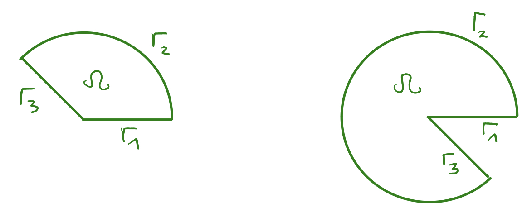
\includegraphics[width=8.94129607765971cm,height=3.69393611439066cm]{k3-2.pdf}}
  \]
  {\hspace{1.7em}}Wir sehen, mit $u (x) = \| x \|^{1 / \alpha} \sin \left(
  \frac{\varphi (x)}{\alpha} \right)$ und $\varphi (x) = \arctan \left(
  \frac{x_2}{x_1} \right)$ ist klassische L{\"o}sung von
  \[ - \Delta u = 0 \text{\quad in } \Omega \text{, \qquad} u (x) =
     \left\{\begin{array}{cl}
       \sin \left( \frac{\varphi (x)}{\alpha} \right), & \text{auf }
       \Gamma_2\\
       0, & \text{auf } \Gamma_1\\
       \| x \|^{1 / \alpha}, & \text{auf } \Gamma_3
     \end{array}\right. \]
  also ist $u$ schwache L{\"o}sung des inhomogenen RWP $\| x \|^{1 / \alpha}
  \sin \pi = 0$ auf $\Gamma_2$ (inh. im Sinne von Nicht-Null auf $\Gamma_2$).
  
  Man kann zeigen: F{\"u}r $\alpha \leqslant 1$ ist $u \in H^2 (\Omega)$;
  falls $\alpha > 1$ ist $u \notin H^2 (\Omega)$.
\end{example*}

\begin{theorem}
  \tmtextbf{(Satz von Friedrichs)}
  
  \tmtextit{Sei $\Omega \subseteq \mathbb{R}^d$ offen, beschr{\"a}nkt mit
  glattem Rand (mindestens $C^2$) oder ein konvexes Lipschitz-Gebiet und $f
  \in L^2 (\Omega)$.
  
  Dann ist das Poisson-RWP mit Dirichlet-Randbedingungen $H^2
  (\Omega)$-regul{\"a}r. }
\end{theorem}

F{\"u}r den Beweis bzgl. glatter Gebiete verweisen wir auf Alt A10.3.

\begin{remark*}
  \
  
  Verallgemeinerung:
  \[ f \in H^{s - 2} (\Omega) \wedge \text{ } \Omega \text{ hat } C^s \text{
     Rand} \hspace{1.5em} \Rightarrow \text{\quad} u \in H^s (\Omega) . \]
\end{remark*}

\begin{example*}
  \
  
  F{\"u}r $d = 2$ und $\Omega \assign \{ x \in \mathbb{R}^2  | \nobracket 1
  \leqslant \| x \| \leqslant 2 \}$ Kreisring ist $u (x) = \ln (\| x \|)$
  gem{\"a}{\ss} Def.2.21 eine klassische L{\"o}sung des inhomogenen RWP
  \[ - \Delta u = 0 \text{\quad in } \Omega, \text{\qquad} u = 0 \text{\quad
     auf } \partial B_1 (0), \text{\qquad} u = \ln (2) \quad \text{auf }
     \partial B_2 (0) \]
  (inhomogen im Sinne von auf $\partial B_2 (0)$ ist $u \neq 0$).
  
  $\Omega$ hat offensichtlich $C^s$-Randbedingung f{\"u}r jedes $s \in
  \mathbb{N}$, dazu ist $f = 0 \in H^m (\Omega)$ f{\"u}r jedes $m \in
  \mathbb{N}$ und $u \in C^{\infty} (\Omega)$, also ist tats{\"a}chlich $u \in
  H^s (\Omega)$ f{\"u}r jedes $s \in \mathbb{N}$. \ 
\end{example*}

Damit schlie{\ss}en wir den Theorieabschnitt ab und kommen zu numerischen
Verfahren.

\

\section{Galerkin-Verfahren}

Wir behandeln zun{\"a}chst das Galerkin-Verfahren, deren \tmtextbf{Grundidee}
lautet: Einschr{\"a}nkung der schwachen Form der PDE auf endlich dimensionalen
Teilraum.

\begin{definition}
  \tmtextbf{(Galerkin-Projektion)}
  
  \tmtextit{}\tmtextit{Sei $a (\bullet, \bullet)$ eine stetige, koerzive
  Bilinearform auf Hilbertraum $V$, $L \in V'$und}
  \begin{equation}
    \forall v \in V : \text{\quad} a (u, v) = L (v) \text{}
  \end{equation}
  \tmtextit{eine schwache Form der PDE.
  
  Sei $V_h \subseteq V$ ein endlich dimensionaler Teilraum.
  
  Gesucht ist ein $u_h \in V_h$, die sogenannte {\underline{diskrete
  L{\"o}sung}} von
  \begin{equation}
    \forall v \in V_h : \text{\quad} a (u_h, v) = L (v) .
  \end{equation}}
\end{definition}

\begin{corollary}
  \tmtextbf{(Existenz, Eindeutigkeit \& Beschr{\"a}nktheit von $u_h$)}
  
  \tmtextit{Die diskrete L{\"o}sung $u_h \in V_h$ von Def. 3.32 existiert
  eindeutig und ist beschr{\"a}nkt durch
  \[ \| u_h \| \leqslant \frac{1}{\alpha} \| L \|_{V'} \]
  mit $\alpha$ der Koerzivit{\"a}tskonstante von $a (\bullet, \bullet)$ auf
  $V$.}
\end{corollary}

\begin{proof}
  \
  
  Da Stetigkeit \& Koerzivit{\"a}t von $a (\bullet, \bullet)$ vererbt sich
  auf Teilr{\"a}ume, ist Lax-Milgram 3.26 auf $V_h$ anwendbar und die Aussage
  folgt analog zu Kor. 3.27. 
\end{proof}

\begin{remark*}
  \
  
  Das ,,$h$`` in $V_h$ indiziert, dass der Raum $V_h$ durch einen
  Diskretisierungsparameter (z.B. Gitterweite) $h \in \mathbb{R}^+$
  charakterisisert wird und es besteht die Hoffung/das Ziel, dass $\lim_{h
  \rightarrow 0} u_h = u$ und die Konvergenz gen{\"u}gend schnell wird. 
\end{remark*}

Wir werden uns mit den folgenden Fragen besch{\"a}ftigen:
\begin{itemizedot}
  \item Wie ist $V_h$ geschickt zu w{\"a}hlen?
  
  \item Existieren a-priori-Fehlerschranken der Form $\| u - u_h \| \leqslant
  C_u h^p$ ?
  
  \item Existieren a-posteriori-Fehlerschranken der Gestalt $\| u - u_h \|
  \leqslant C_{u_h} h^p$ ?
  
  \item Wie stellt man das zugeh{\"o}rige LGS effizient auf?
  
  \item Wie kann man das LGS effizient l{\"o}sen? 
\end{itemizedot}
\begin{lemma}
  \tmtextbf{(Galerkin-Orthogonalit{\"a}t)}
  
  \tmtextit{Seien $u \in V$, $u_h \in V_h$ L{\"o}sungen von (3.6) bzw. (3.7).
  
  Dann gilt
  \[ \forall v \in V_h : \text{\qquad} a (u - u_h, v) = 0. \]}
\end{lemma}

\begin{proof}
  
  \[ a (u - u_h, v) = a (u, v) - a (u_h, v) = L (v) - L (v) = 0 \]
\end{proof}

\begin{remark*}
  {\tmdummy}
  
  \begin{itemizedot}
    \item Falls $a (\bullet, \bullet)$ symmetrisch ist, definiert $a (\bullet,
    \bullet)$ ein Skalarprodukt $\langle \bullet, \bullet \rangle_a$ und Lem.
    3.34 entspricht gerade der orthogonalen Projektion von $V$ auf $V_h$.
    
    \item Falls \ $a (\bullet, \bullet)$ nicht symmetrisch ist, ist die
    Galerkin-Projektion {\underline{nicht}} die orthogonalen Projektion bzgl.
    $\langle \bullet, \bullet \rangle_a$, aber Lem. 3.34 gilt immer noch und
    man spricht immer noch von ,,Galerkin-Orthogonalit{\"a}t``, auch wenn kein
    (offensichliches) Skalarprodukt der Orthogonalit{\"a}t zugrunde liegt. 
  \end{itemizedot}
\end{remark*}

\begin{corollary}
  \tmtextbf{(Reproduktion von L{\"o}sungen)}
  
  \tmtextit{Sei $u \in V$ eine L{\"o}sung der schwachen Form der PDE und $u
  \in V_h$.
  
  Dann gilt $u = u_h$. }
\end{corollary}

\begin{proof}
  \
  
  Mit $u \in V_h$ ist $u - u_h \in V_h$ und daher gilt wegen 3.34
  \[ 0 = a (u - u_h, u - u_h) \geqslant \alpha \| u - u_h \|^2 \geqslant 0 \]
  also $\| u - u_h \| = 0$ und somit $u = u_h$.
\end{proof}

\begin{remark*}
  \
  
  Also ist z.B. $V_h \assign \tmop{span} \{ u \}$ optimaler $1$-dimensionaler
  L{\"o}sungsraum. Dieser ist nat{\"u}rlich so ,,teuer`` zu bestimmen wie $u$,
  daher inpraktikabel. 
\end{remark*}

\begin{theorem}
  \tmtextbf{(Diskretes Problem als LGS)}
  
  \tmtextit{Sei $V_h \subseteq V$ endlich dimensionaler Teilraum mit Basis
  $(\varphi_j)_{j = 1}^n$.
  
  Definiere die ,,Steifigkeitsmatrix`` $A_h = (a_{i j})_{i, j = 1}^n \in
  \mathbb{R}^{n \times n}$ sowie die ,,rechte Seite`` $b_h = (b_i)_{i = 1}^n
  \in \mathbb{R}^n $ durch
  \[ \forall i, j \in \{ 1, \ldots, n \} : \text{{\hspace{3em}}} a_{i j}
     \assign a (\varphi_j, \varphi_i), \text{\qquad} b_i \assign L (\varphi_i)
     \text{{\hspace{3em}}} \]
  und schreibe die L{\"o}sung des LGS
  \begin{equation}
    A_h d = b_h
  \end{equation}
  als $d = (d_j)_{j = 1}^n \in \mathbb{R}^n $.
  
  Dann ist die diskrete L{\"o}sung gegeben durch $u_h = \sum_{j = 1}^n d_j
  \varphi_j$.}
\end{theorem}

\begin{proof}
  \
  
  Wir sollen zeigen, $\sum_{j = 1}^n d_j \varphi_j$ l{\"o}st die schwache
  Form der PDE f{\"u}r alle Testfunktion $v \in V_h$. Wegen $(\varphi_j)_{j =
  1}^n$ Basis von $V_h$ und Linearit{\"a}t von $a (\bullet, \bullet)$ sowie
  $L$ reicht es, die Eigenschaft f{\"u}r $\varphi_i$ zu pr{\"u}fen:
  \[ a \left( \sum_{j = 1}^n d_j \varphi_j, \varphi_i \right) = \sum_{j =
     1}^n a (d_j \varphi_j, \varphi_i) = (A_h d)_i = (b_h)_i = b_i = L
     (\varphi_i) . \]
\end{proof}

\begin{remark*}
  \tmtextbf{(Eigenschaften von $A_h$)}
  \begin{itemizedot}
    \item Mit $a (\bullet, \bullet)$ koerziv folgt $A_h$ positiv definit, denn
    f{\"u}r $\forall d \in \mathbb{R}^d \backslash \{ 0 \}$:
    \[ \langle d, A_h d \rangle = \sum_{i, j = 1}^n d_i d_j a_{i j} = a
       \left( \sum_{i = 1}^n d_i \varphi_i, \sum_{j = 1}^n d_j \varphi_j
       \right) \geqslant \alpha \left\| \sum_{i = 1}^n d_i \varphi_i
       \right\|^2 > 0 \]
    wobei die letzte Stelle gilt, weil $d \neq 0$ und $(\varphi_j)_{j = 1}^n$
    Basis.
    
    \item Falls $a (\bullet, \bullet)$ symmetrisch ist, dann ist $A_h$
    symmetrisch. Dann kann man z.B. das LGS $A_h d = b_h$ durch CG-Verfahren
    l{\"o}sen. 
  \end{itemizedot}
\end{remark*}

\begin{example*}
  \tmtextbf{(Optimales $A_h$)}
  
  Falls $V_h$ gespannt aus Eigenfunktionen des Differentialoperators, bilden
  diese Eigenfunktionen eine optimale Basis bei unbekannter/variabler rechter
  Seite.
  
  Dazu sollen wir zun{\"a}chst eine ,,schwache form`` des Eigenwertproblems
  zum Differentialoperator finden, also:
  
  Finde Eigenfunktion $w \in V \subseteq L^2 (\Omega)$ und Eigenwert
  $\lambda$, s.d.
  \[ \forall v \in L^2 (\Omega) : \text{\quad} a (w, v) = \lambda \langle w,
     v \rangle_{L^2} . \]
  {\hspace{1.7em}}Unter gewissen Voraussetzungen (z.B. $a (\bullet, \bullet)$
  symmetrisch \& $\Omega$ zusammenh{\"a}ngend, sieh Evans K6.5) kann man
  zeigen:
  \begin{itemizedot}
    \item Es existieren nur reelle positive Eigenwerte
    
    \item Es existieren unendlich viele Eigenwerte und die Folge der
    Eigenwerte ist unbeschr{\"a}nkt, d.h. $\exists (\lambda_j)_{j \in
    \mathbb{N}} : \text{\quad} 0 < \lambda_1 \leqslant \lambda_2 \leqslant
    \cdots $\quad$\wedge$\quad$\lim_{j \rightarrow \infty} \lambda_j =
    \infty$.
    
    \item Es existiert eine orthonormale Menge $\{ w_j \}_{j \in \mathbb{N}}$
    in $L^2 (\Omega)$ mit $w_j$ als Eigenfunktion zum Eigenwert $\lambda_j$. 
  \end{itemizedot}
  Aus diem Beispiel von oben k{\"o}nnen wir einen Ansatz formulieren:
  \begin{itemizedot}
    \item W{\"a}hle $k \in \mathbb{N}$, $h \assign \frac{1}{k}$ und $V_h
    \assign \tmop{span} \{ \varphi_1, \ldots, \varphi_k \} \subseteq V$ mit
    $\varphi_j \assign w_j$.
    
    \item F{\"u}r Steifigkeitsmatrix folgt
    \[ a (\varphi_j, \varphi_i) = a (w_j, w_i) = \lambda_j \langle w_j, w_i
       \rangle_{L^2} = \lambda_i \delta_{i j} \]
    also LGS (3.8)
    \[ \left(\begin{array}{ccc}
         \lambda_1 &  & \\
         & \ddots & \\
         &  & \lambda_k
       \end{array}\right) \left(\begin{array}{c}
         d_1\\
         \vdots\\
         d_k
       \end{array}\right) = \left(\begin{array}{c}
         L (w_1)\\
         \vdots\\
         L (w_k)
       \end{array}\right) \]
    und die L{\"o}sung ist dann gegeben durch
    \[ d_j \assign \frac{L (w_j)}{\lambda_j} . \]
  \end{itemizedot}
  {\hspace{1.7em}}Also ist eine optimale Struktur von $A_h$ diagonal, aber das
  Verfahren ist in der Praxis inpraktikabel, da $w_j$, $\lambda_j$ selten
  bekannt sind.
\end{example*}

\begin{example*}
  \tmtextbf{($V_h$ als polynomialer Ansatzraum)}
  
  Sei $d = 1$, $\Omega = (0, 1)$ sowie $a (\bullet, \bullet)$ definiert auf
  $H^1_0 (\Omega)$ durch
  \[ a (u, v) \assign \int_{\Omega} u' v' \mathd \lambda . \]
  {\hspace{1.7em}}Polynom mit Nullrandwerten hat Gestalt $p (x) = x (1 - x) q
  (x)$, daher kann man $k \in \mathbb{N}$, $h \assign \frac{1}{k}$ und $V_h
  \assign \tmop{span} \{ \varphi_1, \ldots, \varphi_k \} \subseteq V$
  w{\"a}hlen wobei $\varphi_j (x) \assign x (1 - x) x^{j - 1} .$
  
  Damit gilt es f{\"u}r die Steifigkeitsmatrix $A_h = (a_{i j})_{i, j = 1}^n$:
  \[ a_{i j} = a (\varphi_j, \varphi_i) = \int_{\Omega} \varphi_j' (x)
     \varphi_i' (x) \mathd \lambda \]
  und i.A. ist $a_{i j} = a (\varphi_j, \varphi_i) \neq 0$.
  
  D.h., die Steifigkeitsmatrix $A_h$ ist i.A. nicht d{\"u}nn besetzt.
  
  Bei sehr gro{\ss}em $k$ ist der Ansatz inpraktikabel wegen
  Speicherproblemen.
  
  Bei ,,m{\"a}{\ss}igem`` $k$ (so $10$ oder $20$) nennt man den Ansatz
  ,,Spektralverfahren``.
\end{example*}

Wir versuchen nun eine Fehlerschranke f{\"u}r $u - u_h$ herzuleiten:

\begin{lemma}
  \tmtextbf{(C{\'e}a)}
  
  \tmtextit{Sei $a (\bullet, \bullet)$ koerzive, stetige Bilinearform auf $V$
  mit Stetigkeitskonstante $\gamma$ und Koerzivit{\"a}tskonstante $\alpha$.
  Sei dazu $L$ eine stetige Linearform.
  
  Dann gilt f{\"u}r L{\"o}sungen $u \in V$ und $u_h \in V_h$ f{\"u}r (3.6)
  bzw. (3.7)
  \[ \| u - u_h \| \leqslant \frac{\gamma}{\alpha} \inf_{v \in V_h}  \| u - v
     \| . \]}
\end{lemma}

\begin{proof}
  \
  
  Sei $v \in V_h$ beliebig, dann gilt
  \begin{eqnarray*}
    \alpha \| u - u_h \|^2 & \leqslant & a (u - u_h, u - u_h)\\
    & = & a (u - u_h, u - v) + a (u - u_h, v - u_h)\\
    & = & a (u - u_h, u - v) + \text{{\hspace{4em}}} 0\\
    & \leqslant & \gamma \| u - u_h \| \cdot \| u - v \|
  \end{eqnarray*}
  wobei die 3. Zeile aus Galerkin-Orthogonalit{\"a}t folgt, und die letzte
  Zeile wegen Stetigkeit von $a (\bullet, \bullet)$.
  
  Insb. gilt die Absch{\"a}tzung f{\"u}r $v \in V_h$ s.d. $\| u - v \|$ das
  Infimum annimmt.
\end{proof}

\begin{remark*}
  \tmtextbf{(Galerkin-Projektion \& Bestapproximation)}
  \begin{itemizedot}
    \item $\inf_{v \in V_h}  \| u - v \|$ auf der rechten Seite von 3.37 ist
    der ,,Bestapproximationsfehler`` gegeben durch orthogonale Projektion
    bzgl. $\langle \bullet, \bullet \rangle_V$ auf $V_h$, und zwar
    unabh{\"a}ngig von $a (\bullet, \bullet)$.
    
    \item $\| u - u_h \|$ ist Galerkin-Projektionsfehler, und dies ist nach
    Lemma von C{\'e}a h{\"o}chstens um einen konstanten, von
    $h$-unabh{\"a}ngigen Fkator $\frac{\gamma}{\alpha}$ schlechter als der
    Bestapproximationsfehler. Man nennt diesen Effekt auch
    ,,Quasi-Optimalit{\"a}t`` der Galerkin-Projektion.
    
    \item Offensichtlich ist ein gutes Konstruktionsprinzip f{\"u}r $V_h$
    gegeben durch:
    
    W{\"a}hle $V_h$ so, dass dieser gute Approximation erm{\"o}glicht, dann
    wird auch $\| u - u_h \|$ klein sein. Formal
    \[ \lim_{n \rightarrow \infty} \inf_{v \in V_h} \| u - v \| = 0 \qquad
       \Rightarrow \text{\qquad} \lim_{n \rightarrow 0} \| u - u_h \| = 0. \]
  \end{itemizedot}
\end{remark*}

\begin{remark*}
  \tmtextbf{(Verbesserung der Schranke f{\"u}r symmetrische Probleme)}
  
  Falls $a (\bullet, \bullet)$ zus{\"a}tzlich symmetrisch ist, so gilt Aussage
  3.37 mit besserem Faktor $\sqrt{\frac{\gamma}{\alpha}}$, denn:
  
  Mit Stetigkeit von $a (\bullet, \bullet)$ ist $\| v \|_a^2 = a (v, v)
  \leqslant \gamma \| v \|^2$, und mit Koerzivit{\"a}t gilt $\alpha \| v \|^2
  \leqslant a (v, v) = \| v \|_a^2$.
  
  Beides kombiniert zusammen ergibt Norm{\"a}quivalenz
  \[ \sqrt{\alpha} \| v \| \leqslant \| v \|_a \leqslant \sqrt{\gamma} \| v
     \| . \]
  {\hspace{1.7em}}Dann gilt \
  \begin{eqnarray*}
    \| u - u_h \|_a^2 & = & a (u - u_h, u - u_h)\\
    & = & a (u - u_h, u - v)\\
    & = & \langle u - u_h, u - v \rangle_a\\
    & \leqslant & \| u - u_h \|_a \cdot \| u - v \|_a
  \end{eqnarray*}
  wobei die zweite Zeile analog wie im Beweis bei C{\'e}a aus
  Galerkin-Orthogonalit{\"a}t folgt, und die letzte Zeile wegen
  Cauchy-Schwarz, also gilt
  \[ \forall v \in V_h : \text{\qquad} \| u - u_h \|_a \leqslant \| u - v
     \|_a . \qquad \]
  {\hspace{1.7em}}Mit Norm{\"a}quivalenz folgt daher
  \[ \| u - u_h \| \leqslant \frac{1}{\sqrt{\alpha}} \| u - u_h \|_a
     \leqslant \frac{1}{\sqrt{\alpha}} \| u - v \|_a \leqslant
     \sqrt{\frac{\gamma}{\alpha}} \| u - v \| \]
  also
  \[ \| u - u_h \| \leqslant \sqrt{\frac{\gamma}{\alpha}} \inf_{v \in V_h} 
     \| u - v \| . \]
\end{remark*}

\begin{remark*}
  \tmtextbf{(Koerzivit{\"a}t wesentlich bei Galerkin-Projektion)}
  
  \tmtextit{}Falls $a (\bullet, \bullet)$ nicht koerziv ist, kann die
  Galerkin-Projektion aus einem regul{\"a}ren System in $V$ ein singul{\"a}res
  System in $V_h$ erzeugen.
  
  Als Beispiel betrachte $V \assign \mathbb{R}^2$, $a (u, v) \assign u^T
  \left(\begin{array}{cc}
    1 & 0\\
    0 & - 1
  \end{array}\right) v$ und $L (v) \assign \left(\begin{array}{cc}
    1 & 1
  \end{array}\right) v$.
  
  Wir sehen, $a (\bullet, \bullet)$ ist nicht koerziv, denn
  \[ \forall \alpha \in \mathbb{R}_+ : \text{\qquad} a (e_2, e_2) = - 1 < 0
     \leqslant \alpha \| e_2 \|^2 = \alpha \]
  aber System in $V$ ist wohlgestellt, da
  \begin{eqnarray*}
    \forall v \in V : \text{ } a (u, v) = L (v) & \text{\quad} \Leftrightarrow
    \text{\quad} & \forall v \in V : \text{ } u^T \left(\begin{array}{cc}
      1 & 0\\
      0 & - 1
    \end{array}\right) v = \left(\begin{array}{cc}
      1 & 1
    \end{array}\right) v\\
    & \text{\quad} \Leftrightarrow \text{\quad} & u^T \left(\begin{array}{cc}
      1 & 0\\
      0 & - 1
    \end{array}\right) = \left(\begin{array}{cc}
      1 & 1
    \end{array}\right)\\
    & \text{\quad} \Leftrightarrow \text{\quad} & u = \left(\begin{array}{c}
      1\\
      - 1
    \end{array}\right)
  \end{eqnarray*}
  (Mehr zu Wohlgestelltheit siehe NUMPDE).
  
  Mit $V_h \assign \tmop{span} \left\{ \varphi_1 \assign
  \left(\begin{array}{c}
    1\\
    1
  \end{array}\right) \right\}$ entsteht jedoch ein singul{\"a}res System, denn
  gem{\"a}{\ss} Satz 3.36 erhalten wir $u_h = d \cdot \varphi_1$ mit $d \in
  \mathbb{R}$ L{\"o}sung des LGS $A_h d = b_h$ wobei
  \begin{eqnarray*}
    A_h = (a_{11}) = a (\varphi_1, \varphi_1) = 0, &  & b_h = L (\varphi_1) =
    2,
  \end{eqnarray*}
  aber das System $0 \cdot d = 2$ ist nicht l{\"o}sbar!
  
  Ausweg daf{\"u}r w{\"a}re Verwendung getrennter Ansatz-\&Testr{\"a}ume,
  also die sogenannte ,,Petrov-Galerkin``-Projektion.
  
  Dabei w{\"a}hlt man $V_h, \tilde{V}_h \subseteq V$ und suche nach $u_h \in
  V_h$ mit der Eigenschaft
  \[ \forall v \in \tilde{V}_h : \text{\qquad} a (u_h, v) = L (v) . \qquad \]
  {\hspace{1.7em}}Man w{\"a}hlt $V_h, \tilde{V}_h$ derart, so dass das
  resultierende projezierte System regul{\"a}r ist, z.B. $\varphi_1 \in
  \mathbb{R}^2 \backslash \left\{ \left(\begin{array}{c}
    1\\
    1
  \end{array}\right) \right\}$ beliebig, $\tilde{\varphi}_1 \assign
  \left(\begin{array}{cc}
    1 & 0\\
    0 & - 1
  \end{array}\right) \varphi_1$, $V_h \assign \tmop{span} \{ \varphi_1 \}$ und
  $\tilde{V}_h \assign \tmop{span} \{ \tilde{\varphi}_1 \}$.
  
  Dann ist $A_h = (a (\varphi_1, \tilde{\varphi}_1)) = \varphi_1^T
  \left(\begin{array}{cc}
    1 & 0\\
    0 & - 1
  \end{array}\right) \tilde{\varphi}_1 = \varphi_1 \left(\begin{array}{cc}
    1 & 0\\
    0 & - 1
  \end{array}\right) \left(\begin{array}{cc}
    1 & 0\\
    0 & - 1
  \end{array}\right) \varphi_1 = \| \varphi_1 \|^2 > 0$ da $\varphi_1 \neq 0$
  und $b_h \assign L (\tilde{\varphi}_1)$, also ist $A_h d = b_h$ eindeutig
  l{\"o}sbar und $u_h = d \varphi_1$ die diskrete L{\"o}sung.
  
  Mit dazu wird in Vorlesung NUMPDE behandelt. 
\end{remark*}

\

\section{Finite Elemente Methode }

Die \tmtextbf{Idee der Finite-Elemente-Methode (FEM)} ist: W{\"a}hle
Galerkin-Verfahren mit st{\"u}ckweise polynomiellen, global stetigen
Ansatzfunktionen, welche lokalen Tr{\"a}ger haben.

Wir betrachten ein einfaches Beispiel:

F{\"u}r $d = 1$, $\bar{\Omega} = [0, 1]$ und $n \in \mathbb{N}$ w{\"a}hlen
wir {\"a}quidistantes Gitter zu Gitterweite $h \assign \frac{1}{n + 1}$ also
$\{ x_i \assign i h \}_{i = 0}^{n + 1}$.

Als Ansatzfunktion definieren wir die ,,H{\"u}tchenfunktion``
\[ \varphi_j (x) \assign \left\{\begin{array}{cl}
     (x - x_{j - 1}) \frac{1}{h}, & x \in [x_{j - 1}, x_j]\\
     1 - (x - x_j) \frac{1}{h}, & x \in [x_j, x_{j + 1}]\\
     0, & \text{sonst}
   \end{array}\right. \]
also hat jedes $\varphi_j$ nur $[x_{j - 1}, x_{j + 1}]$ als Tr{\"a}ger und
,,es sieht so aus wie ein Hut`` wie das Bild darstellt:
\[ 
   \raisebox{-0.00306159669443232\height}{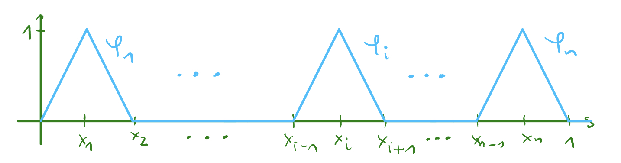
\includegraphics[width=10.4287026105208cm,height=2.74224386724387cm]{k3-3.pdf}}
\]
{\hspace{1.7em}}Au{\ss}erdem sieht man leicht, dass $\varphi_j (x_i) =
\delta_{i j}$ gilt, also bildet $\{ \varphi_j \}_{j = 1}^n$ eine nodale Basis,
und der Ansatzraum $V_h \assign \tmop{span} \{ \varphi_1, \ldots, \varphi_n \}
\subseteq H^1_0 (\Omega)$ ist ein Teilraum der linearen Splines.

F{\"u}r das $1$d-Poisson-Problem $- u'' = f \wedge u (0) = u (1) = 0$ lautet
zun{\"a}chst
\[ a (u, v) \assign \int_{[0, 1]} u' v' \mathd \lambda, \text{\qquad} L (v)
   \assign \int_{[0, 1]} f v \mathd \lambda . \]
{\hspace{1.7em}}Die Ableitung der Ansatzfunktion $\varphi_j$ lautet
\[ \varphi_j' (x) = \left\{\begin{array}{cc}
     \frac{1}{h}, & x \in (x_{j - 1}, x_j)\\
     - \frac{1}{h}, & x \in (x_j, x_{j + 1})\\
     0, & \text{sonst}
   \end{array}\right. \]
oder graphisch dargestellt
\[ 
   \raisebox{-0.00270170439554641\height}{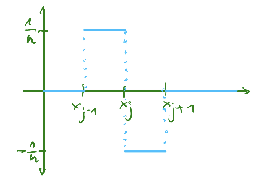
\includegraphics[width=4.47904368358914cm,height=3.10753640299095cm]{k3-4.pdf}}
\]
und damit erhalten wir f{\"u}r die Steifigkeitsmatrix $A = (a_{i j})_{i, j =
1}^n$:
\begin{itemizedot}
  \item Falls $i = j$:
  \[ a_{j j} = a (\varphi_j, \varphi_j) = \int_{[0, 1]} (\varphi'_j)^2 \mathd
     \lambda = \int_{[x_{j - 1}, x_{j + 1}]} \left( \frac{1}{h} \right)^2
     \mathd \lambda = 2 h \left( \frac{1}{h} \right)^2 = \frac{2}{h} . \]
  \item Falls $i = j + 1$:
  \[ a_{j + 1, j} = \int_{[0, 1]} \varphi'_j {\varphi'_{j + 1}}  \mathd
     \lambda = \int_{[x_j, x_{j + 1}]} \frac{1}{h} \left( - \frac{1}{h}
     \right) \mathd \lambda = - h \frac{1}{h^2}  = \frac{- 1}{h} . \]
  \item Falls $i = j - 1$:
  
  Analog zu dem Fall $i = j + 1$, also $a_{j, j - 1} = \frac{- 1}{h}$.
  
  \item Falls $| i - j | \geqslant 2$:
  
  Dann ist $a_{i j} = 0$ da dann $\varphi_i' \varphi_j' = 0$ in allen
  Teilinterwallen. 
\end{itemizedot}
Also erhalten wir
\[ A_h = \frac{1}{h} \left(\begin{array}{cccc}
     2 & - 1 &  & \\
     - 1 & 2 & \ddots & \\
     & \ddots & \ddots & - 1\\
     &  & - 1 & 2
   \end{array}\right), \text{\qquad} b_h = \left(\begin{array}{c}
     \int_{[0, 1]} \varphi_1 f \mathd \lambda\\
     \vdots\\
     \int_{[0, 1]} \varphi_n f \mathd \lambda
   \end{array}\right) \]
{\hspace{1.7em}}Insb. ist $A_h$ eine Tridiagonalmatrix, sehr d{\"u}nn besetzt,
also kein Speicherproblem f{\"u}r gro{\ss}e $n$ falls nur Nicht-Null-Elemente
gespeichert werden.

Dank guter Approximationsf{\"a}higkeit von Splines und des Lemma von C{\'e}a
ergibt gute Approximation der diskrete L{\"o}sung der Galerkin-Projektion
(sp{\"a}ter genauer).

\begin{definition}
  \tmtextbf{(Simplex)}
  
  \tmtextit{Seien $a_0, a_1, \ldots, a_s \in \mathbb{R}^d$ so gew{\"a}hlt,
  dass $\dim \langle a_0, \ldots, a_s \rangle_{\mathbb{R}} = s$ ist, also
  insbes. $s \leqslant d$.
  \begin{enumerateroman}
    \item Dann nennen wir die konvexe H{\"u}lle
    \[ T \assign \tmop{conv} (a_0, \ldots, a_s) = \left\{ x \in \mathbb{R}^d 
       | \nobracket x = \sum_{j = 0}^s \lambda_j a_j, \lambda_j \geqslant 0,
       \sum_{j = 0}^s \lambda_j = 1 \right\} \]
    ein (nicht-degeneriertes) {\underline{$s$-dimensionales Simplex}} in
    $\mathbb{R}^d$. Die Punkte $\{ a_j \}_{j = 0}^s$ hei{\ss}en
    {\underline{Ecken des Simplex}}.
    
    \item F{\"u}r $r \in \{ 0, \ldots, s - 1 \}$ sei $\{ a_0', \ldots, a_r' \}
    \subseteq \{ a_0, \ldots, a_s \}$. Dann ist
    \[ S \assign \tmop{conv} (a_0', \ldots, a_r') \]
    ein {\underline{$r$-dimensionales Seitensimplex}} von $T$ mit
    {\underline{Eckenmenge}}
    \[ \mathscr{E} (s) \assign \{ a_0', \ldots, a_r' \} . \]
    \item Falls $d = s$, $a_0 = e_0 = 0$ und $a_j = e_j$ die Einheitsvektoren
    f{\"u}r $j \in \{ 1, \ldots, d \}$, dann hei{\ss}t $\hat{T} \assign T$ das
    {\underline{Einheitssimplex}} oder {\underline{Referenzelement}} in
    $\mathbb{R}^d$.
  \end{enumerateroman}}
\end{definition}

\begin{remark*}
  {\tmdummy}
  
  \begin{itemizedot}
    \item F{\"u}r $s = 2$ und $d \geqslant 2$ ist $T$ ein Dreieck.
    
    \item F{\"u}r $s = 3$ und $d \geqslant 3$ ist $T$ ein Tetraeder.
    
    \item F{\"u}r $s = 1$ und $d \geqslant 1$ ist $T$ eine Strecke.
    
    \item F{\"u}r $r = 1$ ist $S$ eine Kante und f{\"u}r $r = 0$ ist $S$ eine
    Ecke von $T$.
    \[ 
       \raisebox{-0.0018724400234055\height}{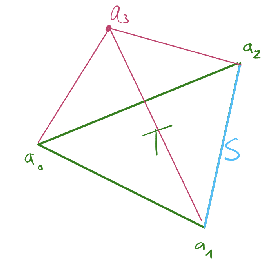
\includegraphics[width=4.47904368358914cm,height=4.48379902925357cm]{k3-5.pdf}}
    \]
  \end{itemizedot}
\end{remark*}

\begin{lemma}
  \tmtextbf{(Baryzentrische Koordinaten)}
  
  \tmtextit{Sei $T = \tmop{conv} (a_0, \ldots, a_s)$ ein $s$-dimensionales
  Simplex in $\mathbb{R}^d$ und $x \in T$.
  
  Dann sind die Zahlen $\{ \lambda_j \}_{j = 0}^s$ mit $x = \sum_{j = 0}^s
  \lambda_j a_j$, $\sum_{j = 0}^s \lambda_j = 1$ und $\lambda_j \geqslant 0$
  eindeutig bestimmt, und sie sind die sogenannte {\underline{Baryzentrischen
  Koordinaten}} (oder ,,lokale Koordinaten``).
  
  Also ist die Abbildung $\lambda : T \rightarrow \mathbb{R}^{s + 1}, x
  \mapsto \{ \lambda_j \}_{j = 0}^s$ wohldefiniert. }
\end{lemma}

\begin{proof}
  \
  
  Die gesuchte $\{ \lambda_j \}_{j = 0}^s$ erf{\"u}llt LGS
  \[ \begin{array}{l}
       \underbrace{\left(\begin{array}{ccc}
         &  & \\
         a_0 & \cdots & a_s\\
         &  & \\
         \hline
         1 & \cdots & 1
       \end{array}\right)} \left(\begin{array}{c}
         \lambda_0\\
         \vdots\\
         \lambda_s
       \end{array}\right) = \left(\begin{array}{c}
         \\
         x\\
         \\
         \hline
         1
       \end{array}\right) .\\
       \text{{\hspace{3.3em}}} \backassign M \in \mathbb{R}^{(d + 1) \times (s
       + 1)}
     \end{array} \]
  {\hspace{1.7em}}Existenz einer L{\"o}sung $\lambda \assign (\lambda_0 \cdots
  \lambda_s)^T$ mit $\lambda_i \geqslant 0$ folgt aus Definition des Simplex
  und $x \in T$.
  
  Eindeutigkeit folgt daraus, dass die Matrix $M$ vollen Spaltenrang besitzt,
  denn Subtraktion der ersten Spalte von $M$ von den {\"U}brigen ergibt eine
  neue Matrix
  \[ \bar{M} \assign \left(\begin{array}{c|ccc}
       &  &  & \\
       a_0 & a_1 - a_0 & \cdots & a_s - a_0\\
       &  &  & \\
       \hline
       1 & 0 & \cdots & 0
     \end{array}\right) \]
  wobei die letzten $s$ Spalten von $\bar{M}$ l.u. sind nach Definition des
  Simplex und die erste Spalte offensichtlich l.u. zu den Anderen sind. 
\end{proof}

\begin{example*}
  \
  
  Betrachte das $2$-dimensionale Einheitssimplex in $\mathbb{R}^3$, also
  \[ 
     \raisebox{-0.00196828447861605\height}{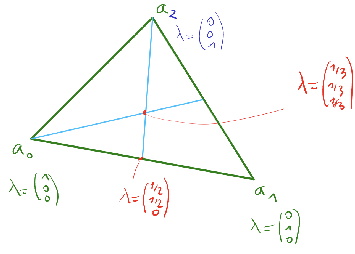
\includegraphics[width=5.96645021645022cm,height=4.26546307228125cm]{k3-6.pdf}}
  \]
  Dabei ist der Punkt $\lambda = \left(\begin{array}{ccc}
    \frac{1}{3} & \frac{1}{3} & \frac{1}{3}
  \end{array}\right)$ der Schwerpunkt des Dreiecks und auch der
  Inkreismittelpunkt, denn er ist der Schnitt der Seitenhalbierend, z.B. via
  $w = \frac{2}{3}$ gilt $\lambda = \left(\begin{array}{ccc}
    0 & 0 & 1
  \end{array}\right) + w \left( \left(\begin{array}{ccc}
    \frac{1}{2} & \frac{1}{2} & 0
  \end{array}\right) - \left(\begin{array}{ccc}
    0 & 0 & 1
  \end{array}\right) \right) .$
\end{example*}

\begin{remark*}
  \
  
  Lemma 3.39 ist sehr praktisch, um zu testen, ob ein Punkt in einem Simplex,
  auf Seitensimplizies, etc., liegt:
  
  Berechnen von $\lambda (x)$, dann {\"U}berpr{\"u}fen ob $\lambda_i
  \geqslant 0$. Falls ja, ist $x \in T$, sonst $x \notin T$.
  
  Anzahl $| \{ \lambda_i  | \nobracket \lambda_i \neq 0 \} | - 1$ ist
  Dimension des Seitensimplex, auf dem $x$ liegt. 
\end{remark*}

\begin{definition}
  \tmtextbf{(Geometrische Ma{\ss}e)}
  
  \tmtextit{F{\"u}r Simplex $T = \tmop{conv} (a_0, \ldots, a_s)$ ist der
  {\underline{Durchmesser}} definiert als
  \[ h_T \assign \tmop{diam} (T) = \max_{x, y \in T} \| x - y \| \]
  und zudem ist der {\underline{Inkugeldurchmesser}} definiert als
  \[ \rho_T \assign 2 \sup \{ R \in \mathbb{R}_+  | \nobracket \exists x_0
     \in T : B_R (x_0) \subseteq T \} . \]
  {\hspace{1.7em}}Wir definieren noch eine Gr{\"o}{\ss}e
  \[ \sigma_T \assign \frac{h_T}{\rho_T} . \]}
\end{definition}

\begin{remark*}
  \
  
  $\sigma_T \geqslant 1$ ist ein Ma{\ss} f{\"u}r die Degeneriertheit eines
  Simplex:
  \begin{itemizedot}
    \item $T$ hat sehr spizite
    Winkel{\hspace{3em}}$\Rightarrow$\quad$\sigma_T$ gro{\ss}
    
    \item $T$ hat sehr {\"a}hnliche Winkel\qquad$\Rightarrow$\quad$\sigma_T$
    klein
  \end{itemizedot}
  \[ 
     \raisebox{-0.00256750996665246\height}{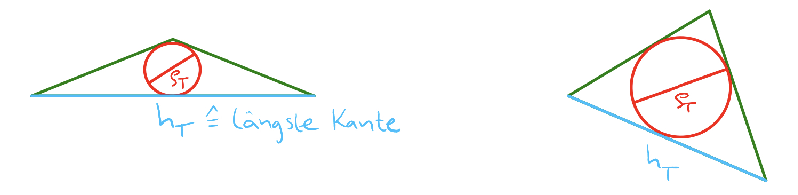
\includegraphics[width=13.4035320739866cm,height=3.26995605404696cm]{k3-7.pdf}}
  \]
  {\hspace{1.7em}}Wir werden sehen: $\sigma_T$ ist invariant unter
  euklidischen Bewegungen \& Skalierungen. 
\end{remark*}

Bei Fehleranalyse \& Implementierung der FEM werden Operationen h{\"a}ufig auf
dem Referenzelement durchgef{\"u}hrt und das Ergebnis auf das gew{\"u}nschte
Simplex transformiert.

\begin{theorem}
  \tmtextbf{(Referenzabbildung)}
  
  \tmtextit{Sei $T = \tmop{conv} (a_0, \ldots, a_s)$ ein $s$-dimensionales
  Simplex in $\mathbb{R}^d$ mit Ecken $\{ a_i \}_{i = 0}^s$ und $\hat{T}
  \subseteq \mathbb{R}^s$ das Referenzelement, d.h. $\hat{T} = \tmop{conv}
  (e_0, e_1, \ldots, e_s)$ wobei $e_0$ der Nullvecktor und $e_i$ die
  kanonischen Einheitsvektoren sind.
  \begin{enumerateroman}
    \item Dann gibt es genau eine Matrix $B \in \mathbb{R}^{d \times s}$ mit
    vollem Spaltenrang und genau ein $t \in \mathbb{R}^d$, sodass es eine
    eindeutige affine Abbildung
    \[ F_T : \hat{T} \rightarrow T, \hat{x} \mapsto B \hat{x} + t \]
    mit der Eigenschaft
    \[ \forall i \in \{ 0, \ldots, s \} : \text{\qquad} F_T (e_j) = a_j
       \text{\qquad} \]
    existiert.
    
    \item F{\"u}r die Norm von $B$ gilt die Absch{\"a}tzung
    \[ \| B \|_2 = \sup_{x \in \mathbb{R}^s \backslash \{ 0 \}} \frac{\| B
       \hat{x} \|_2}{\| \hat{x} \|_2} \leqslant \frac{h_T}{\rho_{\hat{T}}} .
    \]
  \end{enumerateroman}
  {\hspace{1.7em}}Falls $s = d$ gilt, also $B$ regul{\"a}r, dann gilt noch:
  \begin{enumeratealpha}
    \item eine Absch{\"a}tzung f{\"u}r die Norm von $B^{- 1}$, also
    \[ \| B^{- 1} \|_2 \leqslant \frac{{h_{\hat{T}}} }{\rho_T} \]
    \item eine Formel f{\"u}r den Betrag der Determinante von $B$, also
    \[ | \det (B) | = \frac{\lambda^{s - 1} (T)}{\lambda^{s - 1} (\hat{T})}
    \]
    \item sowie eine Absch{\"a}tzung f{\"u}r $\det (B)$, also $\exists c, C
    \in \mathbb{R}_+$ unabh{\"a}ngig von $T$, s.d.
    \[ c \rho_T^d \leqslant | \det (B) | \leqslant C h_T^d . \]
  \end{enumeratealpha}}
\end{theorem}

Den Beweis dazu {\"u}berlassen wir als {\"U}bung.

\

Nun f{\"u}hren wir die numerische Aspekte ein:

\begin{definition}
  \tmtextbf{(Triangulierung)}
  
  \tmtextit{Sei $\Omega \subseteq \mathbb{R}^d$ offen und beschr{\"a}nkt mit
  polygonalem Rand.
  
  Sei $I$ eine endliche Indexmenge.
  
  Wir nennen $\mathcal{T}_h \assign \{ T_i \subseteq \Omega | \nobracket i
  \in I \}$ eine {\underline{zul{\"a}ssige Triangulierung von $\Omega$}},
  g.d.w.
  \begin{itemizedot}
    \item F{\"u}r jedes $i \in I$ ist $T_i$ ein $d$-dimensionales Simplex.
    
    \item {\"U}berdeckung\quad$\bar{\Omega} = \bigcup_{i \in I} T_i$.
    
    \item Nicht-{\"U}berlappung\quad$\forall i, j \in I$ mit $i \neq j$:
    $T^{\circ}_i \cap T^{\circ}_j = \varnothing$.
    
    \item Konformit{\"a}t\quad$\forall i, j \in I$ mit $i \neq j$: die Menge
    $S \assign T_i \cap T_j$ ist entweder eine leere Menge oder ein
    $k$-dimensionaler Seitensimplex von $T_i$ und von $T_j$. 
  \end{itemizedot}
  {\hspace{1.7em}}Wir definieren noch die {\underline{globale Gitterweite}}
  oder {\underline{Feinheit}} von $\mathcal{T}_h$
  \[ h \assign \max_{i \in I} h_{T_i} \]
  den {\underline{minimalen Inkugelradius}}
  \[ \rho \assign \min_{i \in I} \rho_{T_i} \]
  die {\underline{Ecken-oder Knotenmenge}}
  \[ \mathscr{E} (\mathcal{T}_h) \assign \bigcup_{i \in I} \mathcal{E} (T_i)
  \]
  und ein Ma{\ss} f{\"u}r die Degeneriertheit
  \[ \sigma \assign \max_{i \in I} \sigma_{T_i} . \]}
\end{definition}

\begin{remark*}
  {\tmdummy}
  
  \begin{itemizedot}
    \item Eine zul{\"a}ssige Triangulierung hat also keine ,,h{\"a}ngenden
    Knoten``, z.B.
    \[ 
       \raisebox{-0.00229490414741173\height}{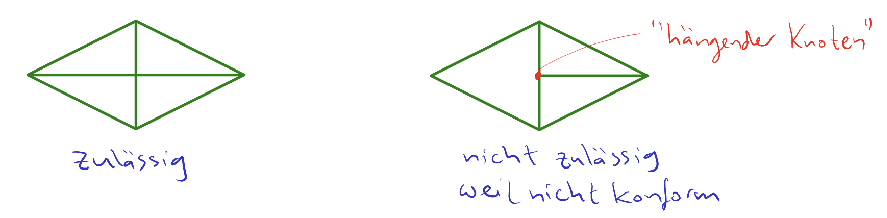
\includegraphics[width=14.8909550045914cm,height=3.65838580611308cm]{k3-8.pdf}}
    \]
    Man kann FEM zwar auch f{\"u}r nichtkonforme (also nicht zul{\"a}ssige)
    Gitter definieren, dies ist aber technisch aufw{\"a}ndiger.
    
    \item Falls $\Omega$ nicht polygonalen Rand hat, kann man mittels sog.
    ,,isoparametrischer Elemente`` den Rand approximieren, d.h. man erlaubt
    nicht affine Referenzabbildung, wie z.B.
    \[ 
       \raisebox{-0.00294028127925207\height}{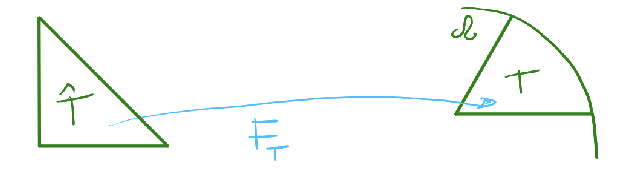
\includegraphics[width=10.4287026105208cm,height=2.85538829857012cm]{k3-9.pdf}}
    \]
    $T$ ist kein Simplex. 
  \end{itemizedot}
\end{remark*}

\begin{definition}
  \tmtextbf{(Lokale Polynomielle R{\"a}ume)}
  
  \tmtextit{Sei $S \subseteq \mathbb{R}^d$ ein $s$-dimensionales Simplex, also
  $s \leqslant d$, und wir definieren den Raum der polynomialen Funktionen bis
  Grad $k \in \mathbb{N}$ auf $S$ durch
  \[ \mathbb{P}_k (S) \assign \left\{ p : S \rightarrow \mathbb{R}  |
     \nobracket p (x) = \sum_{\tilde{\beta} \in \mathbb{N}_0^d, |
     \tilde{\beta} | \leqslant k} \alpha_{\tilde{\beta}} x^{\tilde{\beta}},
     \alpha_{\tilde{\beta}} \in \mathbb{R} \right\} \]
  wobei f{\"u}r $x = (x_1, \ldots, x_d)^T \in \mathbb{R}^d$ und $\tilde{\beta}
  \in \mathbb{N}_0^d$ die Gr{\"o}{\ss}e $x^{\tilde{\beta}} \assign
  x_1^{\tilde{\beta}_1} \cdots x_d^{\tilde{\beta}_d}$ bedeutet.
  
  Damit definieren wir die global stetigen, st{\"u}ckweise polynomiellen
  R{\"a}umen f{\"u}r $\mathcal{T}_h$ durch
  \[ \mathbb{P}_k (\mathcal{T}_h) \assign \{ p \in C^0 (\Omega)  | \nobracket
     \forall i \in I : p |_{T_i} \nobracket \in \mathbb{P}_k (T_i) \} \]
  sowie Teilr{\"a}ume mit Nullrandwerten
  \[ \mathbb{P}_{k, 0} (\mathcal{T}_h) \assign \mathbb{P}_k (\mathcal{T}_h)
     \cap H^1_0 (\Omega) . \]}
\end{definition}

Die R{\"a}ume $\mathbb{P}_k (\mathcal{T}_h)$ werden nachher als
Ansatzr{\"a}ume verwendet.

\begin{lemma}
  \tmtextbf{(Polynom in baryzentrischen Koordinaten)}
  
  Sei $T = \tmop{conv} (a_0, \ldots, a_d)$ ein $d$-dimensionales Simplex in
  $\mathbb{R}^d$.
  \begin{enumerateroman}
    \item Zu $p \in \mathbb{P}_k (T)$ existiert ein $\bar{p} \in \mathbb{P}_k
    (\mathbb{R}^{d + 1})$ der Gestalt
    \[ \bar{p} (\lambda) = \sum_{\beta \in \mathbb{N}_0^{d + 1}, | \beta |
       \in \mathbb{N}_{\leqslant k}} d_{\beta} \lambda^{\beta} \]
    s.d. $p (x) = \bar{p} (\lambda (x))$ f{\"u}r $x \in T$ mit $\lambda : T
    \rightarrow \mathbb{R}^{s + 1}, x \mapsto \{ \lambda_j \}_{j = 0}^s$ den
    baryzentrischen Koordinaten aus 3.39.
    
    \item Zu $\bar{p} \in \mathbb{P}_k (\mathbb{R}^{d + 1})$ ist $\bar{p}
    \circ \lambda = p \in \mathbb{P}_k (T)$.
  \end{enumerateroman}
\end{lemma}

\begin{proof}
  
  \begin{enumerateroman}
    \item Sei $p (x) = \sum_{\tilde{\beta} \in \mathbb{N}_0^d, | \tilde{\beta}
    | \leqslant k} \alpha_{\tilde{\beta}} x^{\tilde{\beta}} =
    \sum_{\tilde{\beta} \in \mathbb{N}_0^d, | \tilde{\beta} | \leqslant k}
    \alpha_{\tilde{\beta}}  \prod_{i = 0}^d x_i^{\tilde{\beta}_i}$.
    
    Mit $x = \sum_{j = 0}^s \lambda_j a_j$ und $a_j = (a_{j i})_{i = 1}^d$
    folgt
    \[ p (x) = \sum_{\tilde{\beta} \in \mathbb{N}_0^d, | \tilde{\beta} |
       \leqslant k} \alpha_{\tilde{\beta}}  \prod_{i = 0}^d \left( \sum_{j =
       0}^d \lambda_j a_{j i} \right)^{\tilde{\beta}_i} \backassign \tilde{p}
       (\lambda) \]
    wobei $\tilde{p}$ nur Monome in $\lambda_j$ der Ordnung h{\"o}chstens $k$
    enth{\"a}lt, daher gilt $p \in \mathbb{P}_k (\mathbb{R}^{d + 1})$ und
    somit $\tilde{p} (\lambda) = \sum_{\beta \in \mathbb{N}_0^{d + 1}, | \beta
    | \leqslant k} \tilde{d}_{\beta} \lambda^{\beta}$ mit geeigneten
    $\tilde{d}_{\beta} \in \mathbb{R}$.
    
    Wir sollen noch den konstanten Anteil via $\sum_{j = 0}^s \lambda_i = 1$
    f{\"u}r jedes $x \in T$ eliminieren, d.h. wir nutzen $\tilde{d}_0 =
    \tilde{d}_0 \cdot 1 = \tilde{d}_0 \sum_{j = 0}^s \lambda_i$ und definiere
    \[ \bar{p} (\lambda) \assign \sum_{\tilde{\beta} \in \mathbb{N}_0^d, |
       \tilde{\beta} | \in \mathbb{N}_{\leqslant k}} d_{\beta} \lambda^{\beta}
    \]
    mit
    \[ d_{\beta} \assign \left\{\begin{array}{cl}
         \tilde{d}_{\beta}, & | \beta | > 1\\
         \tilde{d}_{\beta} + \tilde{d}_0, & | \beta | = 1.
       \end{array}\right. \]
    Dann ist nach Konstruktion $p (x) = \tilde{p} (\lambda (x)) = \bar{p}
    (\lambda (x))$ f{\"u}r jedes $x \in T$.
    
    \item Sei $\bar{p} (\lambda) = \sum_{\beta \in \mathbb{N}_0^{d + 1}, |
    \beta | \leqslant k} d_{\beta} \lambda^{\beta}$.
    
    Gem{\"a}{\ss} Lemma 3.39 ist $\lambda$ L{\"o}sung von
    \[ M \lambda = \left(\begin{array}{c}
         x\\
         1
       \end{array}\right) \]
    f{\"u}r $M \in \mathbb{R}^{(d + 1) \times (s + 1)}$, also
    \[ \lambda = M^{- 1} \left(\begin{array}{c}
         x\\
         1
       \end{array}\right) \backassign \left(\begin{array}{c|c}
         M_1 & m_1
       \end{array}\right) \left(\begin{array}{c}
         x\\
         1
       \end{array}\right) \backassign M_1 x + m_1 \]
    wobei $M_1 \in \mathbb{R}^{(d + 1) \times d}$ und $m_1 \in \mathbb{R}^{d +
    1}$, also eine affin-lineare Abbildung von $x$.
    
    Damit gilt aber $p (x) \assign \bar{p} (\lambda (x)) = \sum_{\beta \in
    \mathbb{N}_0^{d + 1}, | \beta | \leqslant k} d_{\beta}  (M_1 x +
    m_1)^{\beta} \in \mathbb{P}_k (T)$.
  \end{enumerateroman}
\end{proof}

\begin{theorem}
  \tmtextbf{(Lineares Finites Element, Courant-Element)}
  
  \tmtextit{Sei $T = \tmop{conv} (a_0, \ldots, a_d)$ ein $d$-dimensionales
  Simplex in $\mathbb{R}^d$ und $p_0, \ldots, p_d \in \mathbb{R}$.
  
  Dann existiert genau ein $p \in \mathbb{P}_1 (T)$ mit $\forall j \in \{ 0,
  \ldots, d \} : p (a_j) = p_j$.}
\end{theorem}

\begin{remark*}
  {\tmdummy}
  
  \begin{itemizedot}
    \item F{\"u}r $d = 1$ ist es klar wegen eindeutiger Polynominterpolation
    (vgl. NUM I).
    
    \item F{\"u}r $d = 2$ kann man die Situation sch{\"o}n visualisieren
    \[ 
       \raisebox{-0.00232614137669406\height}{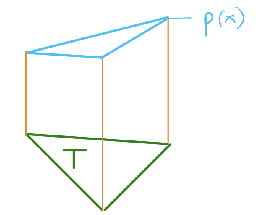
\includegraphics[width=4.47904368358914cm,height=3.60925816607635cm]{k3-10.pdf}}
    \]
    {\hspace{1.7em}}Anschaulich ist es klar, da eine Ebene sich durch $3$
    Punkte in allgemeiner Lage bestimmt.
    
    \item Der allgemeiner Fall f{\"u}r $d \in \mathbb{N}_{\geqslant 3}$ ist
    es nun zu zeigen: 
  \end{itemizedot}
\end{remark*}

\begin{proof}
  \
  
  Sei $d \in \mathbb{N}_{\geqslant 3}$ und $p (x) = c_0 + \sum_{j = 1}^d c_j
  x_j$ also \ $d + 1$ Unbekannte $c_0, \ldots, c_d$ und $d + 1$
  Interpolationsbedingungen $\forall j \in \{ 0, \ldots, d \} : p (a_j) =
  p_j$.
  
  Wir nutzen die Beobachtung
  \[ \forall j \in \{ 0, \ldots, d \} : \text{\quad} p (a_i) = c_0 + \sum_{j
     = 1}^d c_j x_j = \left(\begin{array}{cc}
       a_i^T & 1
     \end{array}\right)^T \left(\begin{array}{c}
       c_1\\
       \vdots\\
       c_d\\
       c_0
     \end{array}\right) = p_i \text{{\hspace{6em}}} \]
  und erhalten damit ein LGS
  \[ \begin{array}{lll}
       \underbrace{\left(\begin{array}{cccc}
         a_{0, 0} & \cdots & a_{0, d} & 1\\
         \vdots & \ddots & \vdots & \vdots\\
         a_{d, 1} & \cdots & a_{d, d} & 1
       \end{array}\right)} & \left(\begin{array}{c}
         c_1\\
         \vdots\\
         c_d\\
         c_0
       \end{array}\right) & = \left(\begin{array}{c}
         p_0\\
         p_1\\
         \vdots\\
         p_d
       \end{array}\right)\\
       \text{{\hspace{1.7em}}} = M^T &  & 
     \end{array} \]
  wobei $M$ der Matrix aus Lemma 3.39 f{\"u}r $s = d$ entspricht.
  
  Dort haben wir gezeigt, dass $M$ vollen Spaltenrang hat.
  
  Also ist $M^T$ regul{\"a}r, somit existiert $\left( c_1 \cdots c_d \enspace
  {c_0}  \right)^T$ eindeutig. 
\end{proof}

\begin{remark*}
  \
  
  F{\"u}r Numerik w{\"a}hlt man konkrete lokale Basis $\Phi = \{ \varphi_0,
  \ldots, \varphi_d \}$ von $\mathbb{P}_1 (T)$, z.B. die nodale Basis zu den
  Ecken und schreibt $p \in \mathbb{P}_1 (T)$ also Linearkombination dieser
  Basis. Die Funktionen $\{ \varphi_j \}_{i = 0}^d$ nennt man
  {\underline{\tmtextit{Formfaktoren}}} (auf Englisch ,,shape functions.``). 
\end{remark*}

\begin{theorem}
  \tmtextbf{(Ex. \& Eind. $\mathbb{P}_1 (\mathcal{T}_h)$
  Interpolationsfunktion)}
  
  \tmtextit{Sei $\Omega \subseteq \mathbb{R}^d$ offen und beschr{\"a}nkt mit
  polygonalem Rand, $\mathcal{T}_h$ eine zul{\"a}ssige Triangulierung von
  $\Omega$ mit $m_1 \assign | \mathscr{E} (\mathcal{T}_h) |$ und Knotenmenge
  $\mathscr{E} (\mathcal{T}_h) = \{ v_i \}_{i = 1}^{m_1}$. Seien $p_1, \ldots,
  p_{m_1} \in \mathbb{R}$.
  
  Dann gibt es genau ein $p \in \mathbb{P}_1 (\mathcal{T}_h)$ s.d. $\forall i
  \in \{ 1, \ldots, m_1 \} : p (v_i) = p_i$.}
\end{theorem}

\begin{proof}
  \
  
  Lokale eindeutige Existenz ist klar nach 3.45, d.h. $\forall T \in
  \mathcal{T}_h$ existiert eindeutiges $p_T \in \mathbb{P}_1 (T)$.
  
  Setze $p (x) : \Omega \rightarrow \mathbb{R}$ mit $p |_T \nobracket \assign
  p_T$ f{\"u}r $\forall T \in \mathcal{T}_h$.
  
  Damit $p$ wohl-definiert ist, m{\"u}ssen wir zeigen, dass die
  {\"u}berlappenden Teile, also am Rand von $T$, keine Mehrdeutigkeit haben,
  also ist die globale Stetigkeit von $p$ noch zu zeigen.
  
  Seien $T$, $T'$ zwei Simplizies mit $S \assign T \cap T'$ und $S$ einem
  $r$-dimensionales Seiten-Simplex von $T$ und $T'$ mit $r \in \mathbb{N}$
  (F{\"u}r $r = 0$ ist nur ein Punkt gemeinsam, und dann ist Stetigkeit klar
  wegen Interpolationsbedingung in $S$).
  
  Als ein $r$-dimensionales Simplex hat $S$ die Eckenmenge $\mathscr{E} (S)
  \subseteq \{ v_i \}_{i = 1}^{m_1}$ mit $| \mathscr{E} (S) | = r + 1$.
  
  Betrachte das Referenzsimplex $\hat{S} \subseteq \mathbb{R}^r$.
  
  Mit 3.45 ist ein Interpolationspolynom $\hat{p} \in \mathbb{P}_1 (\hat{S})$
  durch $r + 1$ Werte eindeutig festgelegt.
  
  Dank Bijektivit{\"a}t $\mathbb{P}_1 (\hat{S}) \cong \mathbb{P}_1 (S)$ ist
  also Interpolationspolynom $p |_S \nobracket \in \mathbb{P}_1 (S)$
  eindeutig, also $p_T |_S \nobracket = p |_S \nobracket = p_{T'} |_S
  \nobracket$, daher ist $p$ stetig {\"u}ber Seitensimplex $S$ hinweg.
\end{proof}

Mit dem Satz folgt sofort Existenz {\"u}ber einer nodalen Basis

\begin{definition}
  \tmtextbf{(Lagrange-Basis, $k = 1$)}
  
  \tmtextit{Sei $\Omega \subseteq \mathbb{R}^d$ offen und beschr{\"a}nkt mit
  polygonalem Rand, $\mathcal{T}_h$ eine zul{\"a}ssige Triangulierung von
  $\Omega$ mit $m_1 \assign | \mathscr{E} (\mathcal{T}_h) |$ und Knotenmenge
  $\mathscr{E} (\mathcal{T}_h) = \{ v_i \}_{i = 1}^{m_1}$.
  
  Dann existieren linear unabh{\"a}ngige Funktionen $\varphi_1, \ldots,
  \varphi_{m_1} \in \mathbb{P}_1 (\mathcal{T}_h)$ mit
  \[ \forall i, j \in \{ 1, \ldots, m_1 \} : \text{\quad} \varphi_i (v_j) =
     \delta_{i j} \text{{\hspace{7em}}} \]
  und $\{ \varphi_i \}_{i = 1}^{m_1}$ spannen $\mathbb{P}_1 (\mathcal{T}_h)$
  auf. D.h. $\dim (\mathbb{P}_1 (\mathcal{T}_h)) = m_1$ und $\{ \varphi_i
  \}_{i = 1}^{m_1}$ ist eine {\underline{nodale}} oder
  {\underline{Lagrange-Basis}} von $\mathbb{P}_1 (\mathcal{T}_h)$.}
\end{definition}

\begin{remark*}
  {\tmdummy}
  
  \begin{itemizedot}
    \item Illustration im Fall $d = 2$:
    \[ 
       \raisebox{-0.00313800479281201\height}{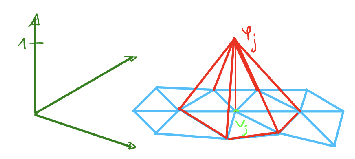
\includegraphics[width=5.96645021645022cm,height=2.67547225501771cm]{k3-11.pdf}}
    \]
    Wir sehen, es ist $\varphi_j (v_i) = \delta_{i j}$ und die
    ,,H{\"u}tchenfunktion`` ist st{\"u}ckweise linear, global stetig und es
    gilt $\tmop{supp} \varphi_j = \bigcup_{i \in \{ j \in I | \nobracket v_j
    \in \mathscr{E} (T_i) \}} T_i$.
    
    \item Geringerer Polynomgrad ($\mathbb{P}_0 (\mathcal{T}_h)$ anstatt
    $\mathbb{P}_1 (\mathcal{T}_h)$) macht bei Forderung nach Stetigkeit keinen
    Sinn, denn $\mathbb{P}_0 (\mathcal{T}_h) = \{ p : \Omega \rightarrow
    \mathbb{R} | \nobracket \exists c \in \mathbb{R} : p \equiv c \}$ besteht
    aus global konstante Funktionen (im Fall $\Omega$ zusammenh{\"a}ngend). \ 
  \end{itemizedot}
\end{remark*}

\begin{theorem}
  \
  
  \tmtextit{Sei $\Omega \subseteq \mathbb{R}^d$ offen und beschr{\"a}nkt mit
  polygonalem Rand, $\mathcal{T}_h$ eine zul{\"a}ssige Triangulierung von
  $\Omega$, und $k \in \mathbb{N}$.
  
  Sei $v : \Omega \rightarrow \mathbb{R}$ mit $v |_{T^{\circ}} \nobracket \in
  C^k (T)$ f{\"u}r jedes $T \in \mathcal{T}_h$.
  
  Dann gilt
  \[ v \in C^{k - 1} (\bar{\Omega}) \qquad \Rightarrow \text{\qquad} v \in H^k
     (\Omega) . \]}
\end{theorem}

\begin{remark*}
  \
  
  Der Satz impliziert insbesondere $\mathbb{P}_1 (\mathcal{T}_h) \subseteq
  H^1 (\Omega)$.
  
  Damit ist dann
  \[ \mathbb{P}_{1, 0} (\mathcal{T}_h) \assign \{ p \in \mathbb{P}_1
     (\mathcal{T}_h)  | \nobracket \forall v_i \in \mathscr{E} (\mathcal{T}_h)
     \cap \partial \Omega : p (v_i) = 0 \} \subseteq H^1_0 (\Omega) \]
  also kann $V_h \assign \mathbb{P}_{1, 0} (\mathcal{T}_h)$ im
  Galerkin-Verfahren verwendet werden.
  
  Dies sind genau die sog. ,,{\underline{lineare Finite-Elemente}}``.
  
  Freiheitsgrade sind also nur die Funktionswerte in den ,,inneren`` Knoten,
  und wir verwenden h{\"a}ufig die Notationen
  \[ m_1 \assign \dim (\mathbb{P}_1 (\mathcal{T}_h)) \text{\qquad
     sowie\qquad} m_{1, 0} \assign \dim (\mathbb{P}_{1, 0} (\mathcal{T}_h)) \]
  wobei wir noch anmerken, dass $m_{1, 0}$ sp{\"a}ter die Gr{\"o}{\ss}e der
  FM-Matrix wird. 
\end{remark*}

\begin{proof}
  (von 3.48)
  
  Es reicht, den Fall $k = 1$ zu zeigen (F{\"u}r $k \in \mathbb{N}_{\geqslant
  2}$ folgt die Behauptung durch Betrachtung der Ableitung der Ordnung $k -
  1$).
  
  Sei $v \in C^{\circ} (\Omega)$ und f{\"u}r $\forall i \in \{ 1, \ldots, d
  \}$ definiere $w_i : \Omega \rightarrow \mathbb{R}$ durch
  \[ w_i |_{T^{\circ}} \nobracket \assign \partial_{x_i} v \]
  (und beliebigen Werten auf $\partial T$).
  
  F{\"u}r $\phi \in C^{\infty}_0 (\Omega)$ und $n = (n_i)_{i = 1}^d$ der
  {\"a}u{\ss}ere Normalenvektor folgt
  \[ \int_{\Omega} w_i \phi \mathd \lambda^d = \sum_{T \in \mathcal{T}_h}
     \int_T \partial_{x_i} v \phi \mathd \lambda^d = \sum_{T \in
     \mathcal{T}_h} \left( - \int_T v \partial_{x_i} \phi \mathd \lambda^d +
     \int_{\partial T} v \phi n_i \mathd \lambda^{d - 1} \right) . \]
  {\hspace{1.7em}}Da $v$ global stetig ist, verschinden die Integrale {\"u}ber
  innere Seitensimplizies, und das Randintegral verschwindet wegen $\phi
  |_{\partial \Omega} \nobracket = 0$.
  
  Somit gilt
  \[ \int_{\Omega} w_i \phi \mathd \lambda^d = - \int_{\Omega} v
     \partial_{x_i} \phi \mathd \lambda^d \]
  also ist $w_i$ die schwache Ableitung von $v$, und $w_i \in L^2 (\Omega)$
  wegen Beschr{\"a}nktheit.
\end{proof}

\begin{definition}
  \tmtextbf{(Lagrange-FEM-Approximation f{\"u}r $k = 1$)}
  
  \tmtextit{Sei $a (\bullet, \bullet)$ stetig und koerziv, $L (\bullet)$
  stetig auf $H^1_0 (\Omega)$.
  
  Sei $\mathcal{T}_h$ eine zul{\"a}ssige Triangulierung von $\Omega$ mit
  nodalen Basisfunktionen $\{ \varphi_i \}_{i = 1}^{m_{1, 0}}$ bzgl. inneren
  Knoten $\mathscr{E} (\mathcal{T}_h) \backslash \partial \Omega \backassign
  \{ v_i \}_{i = 1}^{m_{1, 0}}$.
  
  Setze $V_h \assign \tmop{span} \{ \varphi_i \}_{i = 1}^{m_{1, 0}} =
  \mathbb{P}_{1, 0} (\mathcal{T}_h)$.
  
  Dann ist $u_h \in V_h$ die {\underline{FEM-Approximation}} der PDE g.d.w.
  gilt
  \[ \forall v \in V_h : \text{\qquad} a (u_h, v) = L (v) .
     \text{{\hspace{6em}}} \]}
\end{definition}

Wohlgestelltheit folgt aus Lax-Milgram zusamme mit Galerkin-Projektion eines
koerziven Problems.

\

Im Folgenden behandeln wir das Thema \tmtextbf{Assemblierung des Systems
mittels Quadratur}.

Dazu {\"u}berlegen uns zun{\"a}chst
\begin{itemizedot}
  \item F{\"u}r Aufstellen des LGS, d.h. Berechnung von $A_h$, $b_h$
  (,,Assemblierung``) werden Integrale
  \[ \int_{\Omega} (A (x) \nabla \varphi_i) \bullet \nabla \varphi_j \mathd
     \lambda^d, \text{\quad} \int_{\Omega} f \nabla \varphi_i \mathd
     \lambda^d, \text{\quad} \int_{\Gamma_N} g_N \varphi_i \mathd \lambda^d \]
  durch Quadraturen berechnet / approximiert.
  
  \item Es reicht, Quadraturen auf Referenzelement zu definieren, welche dann
  auf beliebige Simplizies transformiert und zu einer zusammengesetzten
  Quadratur f{\"u}r Gebietsintegral kombiniert werden. 
\end{itemizedot}
\begin{definition}
  \tmtextbf{(Quadratur auf Referenzelement)}
  
  \tmtextit{Sei $\hat{T} \subseteq \mathbb{R}^d$ Einheitssimplex, $l \in
  \mathbb{N}$ Anzahl der St{\"u}tzstellen f{\"u}r Quadratur, $\hat{x}_1,
  \ldots, \hat{x}_l \in \hat{T}$ sowie $w_1, \ldots, w_l \in \mathbb{R}$. Dann
  hei{\ss}t
  \[ \tilde{I} (g) \assign \sum_{i = 1}^l w_i g (\hat{x}_i) \]
  {\underline{Quadratur}} f{\"u}r $g \in C^0 (\hat{T})$.
  
  Schreibe $I (g)$ f{\"u}r das exakte Integral von $g$ auf $\hat{T}$.
  
  Dann hei{\ss}t $\tilde{I}$ {\underline{exakt}} auf $\mathbb{P}_k (\hat{T})$
  oder exakt von Ordnung mindestens $k$, g.d.w. gilt
  \[ \forall g \in \mathbb{P}_k (\hat{T}) : \text{\quad} I (g) = \tilde{I}
     (g) . \text{{\hspace{4em}}} \]}
\end{definition}

\begin{remark*}
  {\tmdummy}
  
  \begin{itemizedot}
    \item \tmtextbf{(Integraltransformation)} F{\"u}r ein $d$-dimensionales
    Simplex $T \subseteq \mathbb{R}^d$ mit Referenzabbildung
    \[ F_T : \hat{T} \rightarrow T, \hat{x} \mapsto B \hat{x} + t \]
    (vgl. 3.41) gilt
    \[ \int_T g (x) \mathd \lambda^d (x) = | \det (B) | \int_{\hat{T}} (g
       \circ F_T) (\hat{x}) \mathd \lambda^d  (\hat{x}) \approx | \det (B) |
       \tilde{I} (g \circ F_T) \backassign \tilde{I}_T (g) \]
    und dabei sieht man leicht
    \begin{eqnarray*}
      \tilde{I}_T  \text{ ist exakt auf } \mathbb{P}_k (T) & \text{\quad}
      \Leftrightarrow \text{\quad} & \tilde{I} \text{ ist exakt auf }
      \mathbb{P}_k (\hat{T}) .
    \end{eqnarray*}
    \item \tmtextbf{(Integration {\"u}ber Differentialausdr{\"u}cke)} Wir
    wissen
    \begin{eqnarray*}
      \varphi \in C^1 (T) & \text{\quad} \Leftrightarrow \text{\quad} &
      \hat{\varphi} \assign \varphi \circ F_T \in C^1 (\hat{T})
    \end{eqnarray*}
    und somit erhalten wir dank der Transformation der Ableitungen
    \[ \nabla_{\hat{x}} \hat{\varphi} (\hat{x}) = (\mathD_{\hat{x}}
       \hat{\varphi} (\hat{x}))^T = (\mathD_x \varphi \cdot \mathD_{\hat{x}}
       F_T)^T = (\mathD_x \varphi \cdot B)^T = B^T \nabla_x \varphi \]
    also die sog. ,,Jacobian inverse transposed``
    \[ \nabla_x \varphi = (B^T)^{- 1} \nabla_{\hat{x}} \hat{\varphi} (\hat{x})
       . \]
    Damit kann man z.B. die Eintr{\"a}ge der Steifigkeitsmatrix umschreiben,
    d.h.f{\"u}r $\forall i, j \in \{ 1, \ldots, m_{1, 0} \}$: \
    \begin{eqnarray*}
      &  & \int_T (\nabla_x \varphi_i (x))^T A (x) \nabla_x \varphi_j (x)
      \mathd \lambda^d (x)\\
      & = & \int_{\hat{T}} (\nabla_{\hat{x}}  \hat{\varphi}_{\hat{i}}
      (\hat{x}))^T B^{- 1} A (\hat{x})  (B^T)^{- 1} \nabla_{\hat{x}}
      \hat{\varphi}_{\hat{j}} (\hat{x}) | \det (B) | \mathd \lambda^d
      (\hat{x})
    \end{eqnarray*}
    f{\"u}r geeignete $\hat{i}, \hat{j} \in \{ 1, \ldots, n_1 \}$ und nodale
    basis $\{ \hat{\varphi}_{\hat{i}} \}_{\hat{i} = 1}^{n_1}$ von
    $\mathbb{P}_1 (\hat{T})$ (Wir k{\"u}mmern uns gleich darum, wie wir die
    ,,geeignete $\hat{i}, \hat{j} \in \{ 1, \ldots, n_1 \}$`` finden
    k{\"o}nnen). 
  \end{itemizedot}
\end{remark*}

\begin{example*}
  Sei $\hat{T}$ ein $d$-dimensionales Referenzelement.
  \begin{itemizedot}
    \item Zun{\"a}chst $d \in \mathbb{N}$ also f{\"u}r beliebige Dimension.
    
    Setze $l \assign 1$ und $\hat{x}_s \assign \frac{1}{d + 1} \left( 1
    \text{ } 1 \cdots 1 \right) \in \mathbb{R}^d$ also der Schwerpunkt von
    $\hat{T}$.
    
    Dann ist
    \[ \tilde{I} (g) \assign \lambda^d (\hat{T}) g (\hat{x}_s) \]
    exakt auf $\mathbb{P}_1 (\hat{T})$.
    
    Dies ist die Mittelpunktsintegration.
    
    \item F{\"u}r besseres Verhalten sei nun $d = 2$.
    
    F{\"u}r $i, j \in \{ 0, 1, 2 \}$ setze $\hat{m}_{i j} \assign \frac{1}{2}
    (e_i + e_j)$ also Kantenmittelpunkte von $\hat{T}$.
    
    Dann ist
    \[ \tilde{I} (g) \assign \frac{1}{3} \lambda^2 (\hat{T})   \sum_{i, j \in
       \{ 0, 1, 2 \}, i < j} g (\hat{m}_{i j}) \]
    exakt auf $\mathbb{P}_2 (\hat{T})$.
    
    \item Sei weiterhin $d = 2$.
    
    F{\"u}r $\hat{x}_s$, $\hat{m}_{i j}$ wie vorhin setzen wir nun
    \[ \tilde{I} (g) \assign \frac{1}{60} \lambda^2 (\hat{T}) \left( 3
       \sum_{i = 0}^2 g (e_i) + 8 \sum_{i, j \in \{ 0, 1, 2 \}, i < j} g
       (\hat{m}_{i j}) + 27 g (\hat{x}_s) \right) \]
    und dies ist exakt auf $\mathbb{P}_3 (\hat{T})$.
  \end{itemizedot}
\end{example*}

\begin{remark*}
  \tmtextbf{(Quadraturen)}
  \begin{itemizedot}
    \item Gebietsintegrale werden dann einfach approximiert durch
    zusammengesetzte Quadraturen:
    \[ \int_{\Omega} g \mathd \lambda^d = \sum_{T \in \mathcal{T}_h}
       \int_{\Omega} g \mathd \lambda^d \approx \sum_{T \in \mathcal{T}_h}
       \tilde{I}_T (g) = \sum_{T \in \mathcal{T}_h} | \det (B_T) | \sum_{i =
       1}^l w_i g (F_T (\hat{x}_i)) . \]
    \item Ordnung der Quadratur sollte der (noch zu diskutierenden)
    Konvergenzordnung der FEM angepasst sein: Quadraturordnung sollte hoch
    genug sein, damit Quadraturfehler nicht Konvergenz der FEM f{\"u}r $h
    \rightarrow 0$ beeintr{\"a}chtigt; Quadraturordnung sollte nicht zu hoch
    sein, um nicht zu viel Rechenzeit in Quadraturen zu verwenden. 
  \end{itemizedot}
\end{remark*}

\begin{remark*}
  \tmtextbf{(Assemblierung {\"u}ber lokale Beitr{\"a}ge)}
  \begin{itemizedot}
    \item Direkte Berechnung der FEM Systemmatrix ist sehr treuer.
    
    Beispiel mit Poisson-Problem:
    \[ \forall i, j \in \{ 1, \ldots, m_{1, 0} \} : \text{\quad} a_{i j} =
       \int_{\Omega} (\nabla \varphi_i)^T \nabla \varphi_j \mathd \lambda^d =
       \sum_{T \in \mathcal{T}_h} \int_T (\nabla \varphi_i)^T \nabla \varphi_j
       \mathd \lambda^d \text{{\hspace{3em}}} \]
    {\hspace{1.7em}}Mit $| \mathscr{E} (\mathcal{T}_h) | = \mathcal{O} (m_{1,
    0})$ betr{\"a}gt der Gesamtaufwand $\mathcal{O} (m_{1, 0}^3)$.
    
    Stattdessen nutzt man ,,Lokalit{\"a}t der Basisfunktion`` \& ,,globale
    Indexabbildung``.
    
    \item \tmtextbf{(Globale Indexabbildung)} Den Zusammenhang zwischen
    lokalen \& globalen Indizes stellt eine entsprechende Abbildung sicher:
    
    Sei $n_1 \assign \dim (\mathbb{P}_1 (\hat{T}))$ mit Basis $\{
    \widehat{\varphi_i} \}_{i = 1}^{n_1}$.
    
    Sei $\hat{g} : \mathcal{T}_h \times \{ 1, \ldots, n_1 \} \rightarrow \{ 1,
    \ldots, m_1 \}$ derart, dass f{\"u}r globale Basis $\{ \varphi_i \}_{i =
    1}^{m_1}$ von $\mathbb{P}_1 (\mathcal{T}_h)$ gilt
    \[ \hat{\varphi}_{\hat{i}} (\hat{x}) = \varphi_i (F_T (\hat{x})) \]
    f{\"u}r $i = \hat{g} (T, \hat{i})$, $\hat{i} \in \{ 1, \ldots, n_1 \}$ und
    $T \in \mathcal{T}_h$.
    
    Hier ist $\hat{i}$ der {\underline{lokale Index}} und i der
    {\underline{globale Index}}.
    
    Damit ist Kenntnis von $\{ \varphi_i \}_{i = 1}^{m_1}$ niemals explizit
    notwendig. Es reicht, eine Basis auf dem Referenzelement zu definieren.
    
    \item Umformulieren der Matrixeintr{\"a}ge
    \begin{eqnarray*}
      a_{i j} & = & \int_{\tmop{supp} (\varphi_i) \cap \tmop{supp}
      (\varphi_j)} (\nabla \varphi_i)^T \nabla \varphi_j \mathd \lambda^d\\
      & = & \sum_{\tmscript{\begin{array}{c}
        T \in \mathcal{T}_h,\\
        T \subseteq \tmop{supp} (\varphi_i) \cap \tmop{supp} (\varphi_j)
      \end{array}}} \int_T (\nabla \varphi_i (x))^T \nabla \varphi_j (x)
      \mathd \lambda^d (x)\\
      & = & \sum_{\tmscript{\begin{array}{c}
        T \in \mathcal{T}_h,\\
        T \subseteq \tmop{supp} (\varphi_i) \cap \tmop{supp} (\varphi_j)
      \end{array}}} \int_{\hat{T}} | \det (B) | (\nabla
      \hat{\varphi}_{\hat{i}} (\hat{x}))^T B^{- 1} (B^T)^{- 1} \nabla
      \hat{\varphi}_{\hat{j}} (\hat{x}) \mathd \lambda^d (\hat{x})\\
      & = : & \sum_{\tmscript{\begin{array}{c}
        T \in \mathcal{T}_h,\\
        T \subseteq \tmop{supp} (\varphi_i) \cap \tmop{supp} (\varphi_j)
      \end{array}}} a_{\hat{i} \hat{j}, T}
    \end{eqnarray*}
    mit $\hat{i}, \hat{j} \in \{ 1, \ldots, n_1 \}$ derart, dass $\hat{g} (T,
    \hat{i}) = i$ und $\hat{g} (T, \hat{j}) = j$ gilt.
    
    \item Statt Schleife {\"u}ber $i, j$, f{\"u}hren wir Schleife {\"u}ber $T
    \in \mathcal{T}_h$ aus, um mit Schleife {\"u}ber $\hat{i}, \hat{j}$ lokale
    Steifigkeitsmatrix $A_{h, T} \in \mathbb{R}^{n_1 \times n_1}$ zu berechnen
    \[ A_{h, T} \assign (a_{\hat{i} \hat{j}, T})_{\hat{i}, \hat{j} = 1}^{n_1}
       . \]
    \item ``Assembliere`` globale Steifigkeitsmatrix $A_h$ durch Addition der
    lokalen Beitr{\"a}ge in entsprechende Eintr{\"a}ge von $A_h$:
    \[ \begin{array}{l}
         A_h = 0\\
         \tmop{for} \enspace T \in \mathcal{T}_h :\\
         \text{\qquad} \tmop{calculate} \enspace A_{h, T}\\
         \text{\qquad} \tmop{for} \enspace \hat{i}, \hat{j} \in \{ 1, \ldots,
         n_1 \} :\\
         \text{{\hspace{4em}}} (A_h)_{\hat{g} (T, \hat{i}), \hat{g} (T,
         \hat{j})} \plusassign (A_{h, T})_{\hat{i}, \hat{j}} .
       \end{array} \]
    \item Gesamtkomplexit{\"a}t betr{\"a}gt dann $\mathcal{O} (| \mathscr{E}
    (\mathcal{T}_h) | \cdot n_1^2) = \mathcal{O} (m_{1, 0} \cdot n_1^2)$ und
    dies ist wesentlich schneller als $\mathcal{O} (m_{1, 0}^3)$.
    
    \item {\"A}hnlich ist Assemblierung der rechten Seite m{\"o}glich, sogar
    ohne zus{\"a}tzliche Schleife {\"u}ber $T$, d.h. simultan mit $A_h$ wird
    $b_h$ auch berechnet.
    
    Anders ausgedr{\"u}ckt: ,,Einzelner Gitterlauf`` reicht zur Assemblierung
    des Systems $A_h$, $b_h$.
  \end{itemizedot}
\end{remark*}

\begin{example*}
  Basen auf Referenzelemente f{\"u}r
  \begin{itemizedot}
    \item $d = 1$, $\hat{T} = [0, 1]$, $n_1 = 2$
    \[ 
       \raisebox{-0.00258622431454953\height}{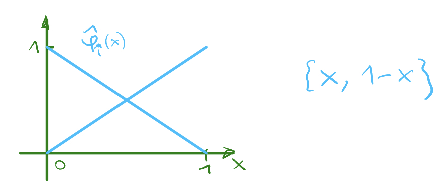
\includegraphics[width=7.45387314705497cm,height=3.24629410993047cm]{k3-12.pdf}}
    \]
    \item $d = 2$, $\hat{T}$ Einheitsdreieck, $n_1 = 3$
    \[ 
       \raisebox{-0.00216522529761275\height}{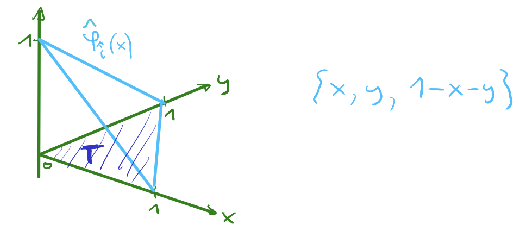
\includegraphics[width=8.94129607765971cm,height=3.87749245703791cm]{k3-13.pdf}}
    \]
  \end{itemizedot}
\end{example*}

\begin{remark*}
  \tmtextbf{(Struktur von $A_h$)}
  
  {\underline{D{\"u}nnbesetztheit}}, also sobald $\tmop{supp} (\varphi_i) \cap
  \tmop{supp} (\varphi_j)$ eine Nullmenge in $\mathbb{R}^d$ ist, gilt
  $(A_h)_{i, j} = 0$. Konkreter:
  
  Sei $r$ maximale Kantenzahl aus einem Knoten, z.B. f{\"u}r $r = 5$ sieht es
  so aus
  \[ 
     \raisebox{-0.00321503026649587\height}{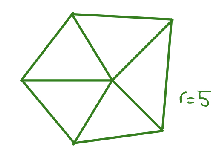
\includegraphics[width=3.7353404171586cm,height=2.61137347500984cm]{k3-14.pdf}}
  \]
  {\hspace{1.7em}}Dann existieren in jeder Zeile von $A_h$ h{\"o}chstens $r +
  1$ Nicht-Null-Eintr{\"a}ge.
  
  Dies muss bei Implementierung durch Sparse-Matrizen f{\"u}r
  Speichereffizienz ber{\"u}cksichtigt werden, insbesondere muss bei
  Verfeinerung darauf geachtet werden, dass $r$ nicht unbegrenzt w{\"a}chst. \
  
\end{remark*}

\

\section{FEM-Konvergenz/Fehleranalyse}

Wir schildern zun{\"a}chst den \tmtextbf{groben Plan der Fehleranalyse}:

Gegeben ist $I_h : V \rightarrow V_h$ ein linearer Interpolationoperator mit
Approximationsg{\"u}te $\| u - I_h u \| \leqslant C \cdot h^p$ mit
m{\"o}glichst gr{\"o}{\ss}en $p$. Dann folgt mit C{\'e}a f{\"u}r
Galerkin-Projektion
\[ \| u - u_h \| \leqslant \frac{\gamma}{\alpha} \inf_{v \in V_h} \| u - v \|
   \leqslant \frac{\gamma}{\alpha} \| u - I_h u \| \leqslant
   \frac{\gamma}{\alpha} C \cdot h^p \]
also Konvergenz f{\"u}r $h \rightarrow 0$, und zudem sieht man auch die
Konvergenzordnung \& Fehlerschranke.

Wir sollen uns einige {\"U}brelegung zum linearen Interpolationsoperator
machen:

Sei $\Omega \subseteq \mathbb{R}^d$ polygonal berandet, $\mathcal{T}_h$
Triangulierung von $\Omega$ und $I_h$ ein Lagrange-Interpolationsoperator.

Damit $I_h : H^m (\Omega) \rightarrow \mathbb{P}_1 (\mathcal{T}_h)$ sinnvoll
definiert ist, muss $H^m (\Omega)$ Punktauswertungen erlauben, d.h. $v \in H^m
(\Omega)$ muss einen stetigen Repr{\"a}sentanten $\tilde{v} \in C^0 (\Omega)$
besitzen, d.h. $\| v - \tilde{v} \|_{H^m (\Omega)} = 0$, damit Punktauswertung
von $v$ als Punktauswertung von $\tilde{v}$ definiert werden kann.

Erinnerung:
\begin{itemizedot}
  \item F{\"u}r $d = m = 1$ hat $v \in H^1 (\Omega)$ stetigen
  Repr{\"a}sentanten.
  
  \item Allgemeiner gilt der 2. Sobolev'sche Einbettungssatz:
  
  F{\"u}r Sobolev-Index $m - \frac{d}{p} > 0$ hat $v \in H^{m, p} (\Omega)$
  stetigen Repr{\"a}sentanten.
\end{itemizedot}
Sei im Folgenden $d, m$ derart, dass $I_h$ wohldefiniert ist.

\begin{definition}
  \tmtextbf{(Gebrochene Normen)}
  
  \tmtextit{Sei $\mathcal{T}_h$ eine Triangulierung von $\Omega$.
  
  F{\"u}r $m \geqslant 0$ definieren wir gitterabh{\"a}ngige Normen \&
  R{\"a}ume
  \[ H^m (\mathcal{T}_h) \assign \{ v : \Omega \rightarrow \mathbb{R}  |
     \nobracket \forall T \in \mathcal{T}_h : v |_T \nobracket \in H^m (T) \}
  \]
  mit Seminorm
  \[ | v |_{H^m (\mathcal{T}_h)} \assign \sqrt{\sum_{T \in \mathcal{T}_h} | v
     |^2_{H^m (T)}} \]
  und Norm \
  \[ | | v | |_{H^m (\mathcal{T}_h)} \assign \sqrt{\sum_{T \in \mathcal{T}_h}
     | | v | |^2_{H^m (T)}} . \]}
\end{definition}

\begin{remark*}
  Man sieht leicht, dass es gilt
  \begin{itemizedot}
    \item $H^m (\Omega) \subseteq H^m (\mathcal{T}_h)$.
    
    \item $v \in H^m (\Omega)$\quad$\Rightarrow$\quad$\| v \|_{H^m
    (\mathcal{T}_h)} = \| v \|_{H^m (\Omega)}$.
    
    \item $H^0 (\mathcal{T}_h) = L^2 (\mathcal{T}_h) \assign L^2 (\Omega)$.
  \end{itemizedot}
\end{remark*}

\begin{theorem}
  \tmtextbf{(Interpolationsabsch{\"a}tzung)}
  
  \tmtextit{Sei $\mathcal{T}_h$ zul{\"a}ssige Triangulierung von $\Omega
  \subseteq \mathbb{R}^d$ und $m \in \{ 0, 1, 2 \}$.
  
  Seien dazu $\sigma_{\max}, h_{\max} \in \mathbb{R}_+$ s.d. f{\"u}r jedes $T
  \in \mathcal{T}_h$ gilt $\sigma_T \leqslant \sigma_{\max}$ und $h_T
  \leqslant h_{\max}$.
  
  Sei $I_h : H^2 (\Omega) \rightarrow \mathbb{P}_1 (\mathcal{T}_h)$ der
  Lagrange-Interpolationsoperator.
  
  Dann existiert ein $C = C (\Omega, \sigma_{\max}, h_{\max}, m, d)$ s.d. es
  gilt
  \begin{equation}
    \forall u \in H^2 (\Omega) : \text{\qquad} \| u - I_h u \|_{H^m
    (\mathcal{T}_h)} \leqslant C \cdot h^{2 - m} | u |_{H^2 (\Omega)} .
  \end{equation}}
\end{theorem}

F{\"u}r den Beweis dieses Satzes verweisen wir auf Satz 6.4 in Braess: FEM.

\begin{remark*}
  \
  
  Beispielsweise sind die Eigenschaften f{\"u}r $d = 2$ und $m = 2$
  sch{\"o}n:
  \begin{itemizedot}
    \item Mit Sobolev-Index $m - \frac{d}{p} = 2 - \frac{2}{2} = 1 > 0$ ist
    $I_h : H^2 (\Omega) \rightarrow \mathbb{P}_1 (\mathcal{T}_h)$
    wohldefiniert wegen sinnvoller Punktauswertung.
    
    \item F{\"u}r die Absch{\"a}tzung gilt dann $\| u - I_h u \|_{H^2
    (\mathcal{T}_h)} \leqslant C \cdot h^{2 - 2} | u |_{H^2 (\Omega)} = C | u
    |_{H^2 (\Omega)} .$
  \end{itemizedot}
\end{remark*}

Der Satz 3.52 ist die wesentliche Aussage, welche wir auf Gittersequenz
anwenden, um Konvergenz von FEM sicherzustellen. Nun definieren wir
Gittersequenzen:

\begin{definition}
  \tmtextbf{(Gittersequenz-Charakterisierung)}
  
  \tmtextit{Eine Folge $\{ \mathcal{T}_i \}_{i \in \mathbb{N}}$ von
  Triangulierungen mit $h_i \assign h (\mathcal{T}_i)$ und $\lim_{i
  \rightarrow 0} h_i = 0$ hei{\ss}t
  \begin{itemizedot}
    \item {\underline{nicht-entartet}}, g.d.w. es gilt
    \[ \exists \sigma_{\max} \in \mathbb{R}_+ \forall i \in \mathbb{N}
       \forall T \in \mathcal{T}_i : \text{\qquad} \sigma_T =
       \frac{h_T}{\rho_T} \leqslant \sigma_{\max} \]
    \item {\underline{quasi-uniform}}, g.d.w. es gilt
    \[ \exists \sigma_{\max} \in \mathbb{R}_+ \forall i \in \mathbb{N}
       \forall T \in \mathcal{T}_i : \text{\qquad} \sigma_T =
       \frac{h_i}{\rho_T} \leqslant \sigma_{\max} . \]
  \end{itemizedot}}
\end{definition}

\begin{remark*}
  \tmtextbf{(Illustration von Def. 3.53.)}
  \begin{itemizedot}
    \item Eine Gittersequenz wie
    \[ 
       \raisebox{-0.00372477411281992\height}{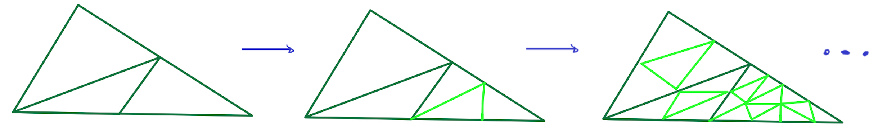
\includegraphics[width=14.8909550045914cm,height=2.25400104945559cm]{k3-15.pdf}}
    \]
    also zun{\"a}chst nur rechtes Dreieck verfeinernd, dann alle Dreiecke
    vierteilend, dann nur rechts, dann alle{\textdots} ist nicht-entartet,
    aber nicht quasi-uniform, denn $\rho_T$ f{\"a}llt schneller ab als $h_i$.
    
    \item Eine Gittersequenz wie
    \[ 
       \raisebox{-0.00353439825489086\height}{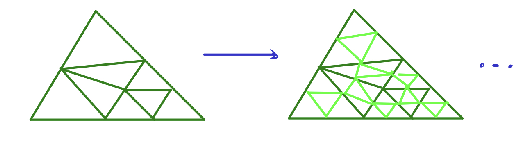
\includegraphics[width=8.94129607765971cm,height=2.37540994359176cm]{k3-16.pdf}}
    \]
    also immer alle Dreicke vierteilend ist quasi-uniform und auch
    nicht-entartet, d.h. $\exists C : h_T \leqslant h_i \leqslant C \cdot
    h_T$.
  \end{itemizedot}
\end{remark*}

\begin{remark*}
  {\tmdummy}
  
  \begin{itemizedot}
    \item ``Quasi-uniform`` impliziert ,,nicht-entartet``.
    
    \item Nicht-entartete gitter lassen auch lokal verfeinerte Gitter zu.
    
    \item In nicht-entarteten Gittern sind innere Winkel durch $\phi_{\min} >
    0$ nach unten beschr{\"a}nkt. 
  \end{itemizedot}
\end{remark*}

\begin{corollary}
  \tmtextbf{(Konvergenz der Interpolation)}
  
  \tmtextit{Sei $\{ \mathcal{T}_i \}_{i \in \mathbb{N}}$ eine Folge
  nicht-entarteter Triangulierungen, $h_{\max} \assign \max_{i \in \mathbb{N}}
  h_i$ und $\lim_{i \rightarrow \infty} h_i = 0$.
  
  F{\"u}r jedes $i \in \mathbb{N}$ sei $I_{h_i} : H^2 (\Omega) \rightarrow
  \mathbb{P}_1 (\mathcal{T}_i)$ der Lagrange-Interpolationsoperator.
  
  Dann gilt
  \[ \forall m \in \{ 0, 1 \} \forall u \in H^m (\Omega) : \text{\quad}
     \lim_{i \rightarrow \infty} \| u - I_{h_i} u \|_{H^m (\mathcal{T}_i)} =
     0. \]}
\end{corollary}

\begin{proof}
  \
  
  Es ist $h_i^{2 - m} \leqslant h_{\max}^{1 - m} h_i$ und daher $0 \leqslant
  \lim_{i \rightarrow \infty} h_i^{2 - m} < h_{\max}^{1 - m} \lim_{i
  \rightarrow \infty} h_i \leqslant h_{\max}^{1 - m} \cdot 0 = 0$.
  
  In (3.9) ist $C$ unabh{\"a}ngig vom Index $i$, daher erhalten wir mit 3.52
  \[ \lim_{i \rightarrow \infty} \| u - I_{h_i} u \|_{H^m (\mathcal{T}_i)}
     \leqslant \lim_{i \rightarrow \infty} C \cdot h_i^{2 - m} | u |_{H^2
     (\Omega)} = C | u |_{H^2 (\Omega)} \lim_{i \rightarrow \infty} h_i^{2 -
     m} = 0. \]
\end{proof}

\begin{theorem}
  \tmtextbf{(FEM a-priori Fehlerschranke in $H^1$)}
  
  \tmtextit{Sei $\Omega \subseteq \mathbb{R}^d$ beschr{\"a}nkt und polygonal
  berandet.
  
  Sei $a (\bullet, \bullet)$ koerziv und stetig, $L (\bullet)$ stetig auf
  $H^1_0 (\Omega)$, und $u \in H^1_0 (\Omega)$ die eindeutige schwache
  L{\"o}sung der PDE schwacher Form bzgl. $a (\bullet, \bullet)$ und $L
  (\bullet)$.
  
  Sei $\mathcal{T}_h$ eine zul{\"a}ssige Triangulierung von $\Omega$.
  
  Seien dazu $\sigma_{\max}, h_{\max} \in \mathbb{R}_+$ s.d. f{\"u}r jedes $T
  \in \mathcal{T}_h$ gilt $\sigma_T \leqslant \sigma_{\max}$ und $h_T
  \leqslant h_{\max}$.
  
  Sei $u_h \in V_h \assign \mathbb{P}_{1, 0} (\mathcal{T}_h)$ die
  Lagrange-FEM-L{\"o}sung.
  
  Falls $u \in H^2 (\Omega)$ ist, so existiert ein $\tilde{C}$=$\tilde{C}
  (\Omega, \sigma_{\max}, h_{\max}, m, d)$ mit
  \[ \| u - u_h \|_{H^1 (\Omega)} \leqslant \tilde{C} \cdot h \| u \|_{H^2
     (\Omega)} . \]}
\end{theorem}

\begin{proof}
  Wir erhalten eine Absch{\"a}tzungskette
  \[ \| u - u_h \|_{H^1 (\Omega)} \leqslant \frac{\gamma}{\alpha} \inf_{v \in
     V_h} \| u - v \|_{H^1 (\Omega)} \leqslant \frac{\gamma}{\alpha} \| u -
     I_h u \|_{H^1 (\Omega)} \leqslant \frac{\gamma}{\alpha} C \cdot h  | u
     |_{H^2 (\Omega)} \leqslant \frac{\gamma}{\alpha} C  \cdot h {\| u \|_{H^2
     (\Omega)}}  \]
  wobei die erste Ungleichheit wegen Lemma von C{\'e}a, und die dritte
  Ungleichheit wegen $\| \bullet \|_{H^1 (\Omega)} = \| \bullet \|_{H^1
  (\mathcal{T}_h)}$ und 3.52 mit $m = 1$.
  
  Deswegen gilt die Behauptung mit $\tilde{C} \assign \frac{\gamma}{\alpha}
  C$.
\end{proof}

\begin{corollary}
  \tmtextbf{(Konvergenz von FEM)}
  
  \tmtextit{Sei $\{ \mathcal{T}_i \}_{i \in \mathbb{N}}$ eine Folge von
  nicht-entarteter zul{\"a}ssigen Triangulierungen mit $h_i \assign h
  (\mathcal{T}_i)$, $\sigma_i \assign \sigma (\mathcal{T}_i)$, $h_{\max}
  \assign \sup_{i \in \mathbb{N}} h_i$, $\sigma_{\max} \assign \sup_{i \in
  \mathbb{N}} \sigma_i$ und $\lim_{i \rightarrow 0} h_i = 0$.
  
  Seien die weiteren Voraussetzungen von 3.55 erf{\"u}llt.
  
  Dann gilt in $H^1 (\Omega)$
  \[ \lim_{i \rightarrow \infty} u_{h_i} = u. \]}
\end{corollary}

\begin{remark*}
  \
  
  F{\"u}r lineare FEM braucht man die $H^2 (\Omega)$-Regularit{\"a}t, dann
  gilt Konvergenz erster Ordnung in $h$ bzgl. $H^1$-Norm, also
  \[ \| u - u_h \|_{H^1 (\Omega)} \leqslant C \cdot h \| u \|_{H^2 (\Omega)}
     \leqslant C \cdot C_R h \| f \|_{L^2 (\Omega)} \]
  wobei erste Ungleichheit aus 3.55 folgt, die Zweite aus 3.31 Satz von
  Friedrichs. 
\end{remark*}

\begin{remark*}
  \tmtextbf{(Hinsicht aus einem numerischen Beispiel)}
  
  Bei einem numerischen Beispiel (siehe Vorlesung 28 gegen Ende) kann man
  tats{\"a}chlich Konvergenzordnung $1$ bzgl. $\| \bullet \|_{H^1}$-Fehler
  beobachten, zudem interessanterweise aber noch Konvergenzordnung $2$ bzgl.
  $\| \bullet \|_{L^2}$-Fehler. Dies wird in Vorlesung ENUMPDE in WS22/23
  behandelt. 
\end{remark*}

\begin{remark*}
  \tmtextbf{(Method of Lines)}
  
  F{\"u}r zeitabh{\"a}ngige PDEs lassen sich Kapitel 1 \& Kapitel 2/3
  verbunden.
  
  Bpsw. kann man ein Anfangsrandwertproblem
  \begin{eqnarray*}
    \partial_t u - \Delta_x u = f &  & \text{in } (0, T) \times \Omega\\
    u (0, x) = u_0 (x) &  & x \in \Omega\\
    u (t, x) = g (t, x) &  & x \in \partial \Omega
  \end{eqnarray*}
  ,,semi-diskretisieren``, also
  \begin{itemizedot}
    \item F{\"u}hre eine Ortsdiskretisierung gem{\"a}{\ss} Kapitel 2/3 mit
    inneren Knoten $\{ x_i \}_{i = 1}^n \subseteq \Omega$ durch.
    
    \item Finde $U (t) = (U_i (t))_{i = 1 }^n$ mit $U_i (t) \approx u (t,
    x_i)$ und $U_i (0) = u_0 (x_i)$, d.h. L{\"o}sung entlang ,,Linien`` im
    Orts-Zeit-Raum
    \begin{equation}
      \frac{\mathd}{\mathd t} U (t) - A_h U (t) = f_h (t)
    \end{equation}
    mit geeignetem $A_h$, z.B. FD-Matrix und $f_h$ Quellterm plus Randwerte.
    
    \item (3.10) ist ein ODE-System, das mit Kapitel 1 numerisch gel{\"o}st
    werden kann.
    
    \item Stabilit{\"a}tsbedingungen bzw. Konvergenzordnung ergeben h{\"a}ufig
    Zusammenhang von Zeit-\&Ortsdiskretisierungsparameter $\tau$ bzw. $h$. \ 
  \end{itemizedot}
  {\hspace{1.7em}}Details dazu werden in Vorlesung ENUMPDE in WS22/23
  behandelt. \ 
\end{remark*}

\

\

\tmtextbf{Ende der Vorlesung}

\end{document}
